\documentclass[9pt]{article}
\usepackage[english]{babel}
\usepackage{amsmath,amsthm}
\usepackage{amsfonts}
\usepackage{graphicx}
\usepackage[margin=0.2in]{geometry}
\newcommand{\setlinespacing}[1]{\setlength{\baselineskip}{#1 \defbaselineskip}}
\newcommand{\doublespacing}{\setlength{\baselineskip}{2.0 \defbaselineskip}}
\newcommand{\singlespacing}{\setlength{\baselineskip}{\defbaselineskip}}
\newcommand{\A}{{\cal A}}
\newcommand{\h}{{\cal H}}
\newcommand{\s}{{\cal S}}
\newcommand{\W}{{\cal W}}
\newcommand{\BH}{\mathbf B(\cal H)}
\newcommand{\KH}{\cal  K(\cal H)}
\newcommand{\Real}{\mathbb R}
\newcommand{\Complex}{\mathbb C}
\newcommand{\Field}{\mathbb F}
\newcommand{\RPlus}{[0,\infty)}
\newcommand{\norm}[1]{\left\Vert#1\right\Vert}
\newcommand{\essnorm}[1]{\norm{#1}_{\text{\rm\normalshape ess}}}
\newcommand{\abs}[1]{\left\vert#1\right\vert}
\newcommand{\set}[1]{\left\{#1\right\}}
\newcommand{\seq}[1]{\left<#1\right>}
\newcommand{\eps}{\varepsilon}
\newcommand{\To}{\longrightarrow}
\newcommand{\RE}{\operatorname{Re}}
\newcommand{\IM}{\operatorname{Im}}
\newcommand{\Poly}{{\cal{P}}(E)}
\newcommand{\EssD}{{\cal{D}}}
\newcommand{\field}[1]{\mathbb{#1}}
\newcommand{\C}{\field{C}}
\newcommand{\R}{\field{R}}
\newcommand{\script}[1]{\mathcal{#1}}
\newcommand{\fall}{\; \forall \;}
\newcommand{\exts}{\; \exists \;}
\newcommand{\mbf}[1]{\mathbf{#1}}
\newcommand{\binomial}[2]{\biggl( \begin{array}{c}  #1 \\ #2  \\ \end{array} \biggr) }
\newcommand{\fderiv}[2]{ \frac{d}{ d #1} \: #2}
\newcommand{\sderiv}[2]{ \frac{d^2}{ d^2 #1} \: #2}
\newcommand{\pfderiv}[2]{ \frac{\partial}{ \partial #1} \: #2}
\newcommand{\psderiv}[2]{ \frac{\partial^2}{ \partial^2 #1} \: #2}
\newcommand{\mat}[1]{\mathbf{#1}}
\DeclareSymbolFont{AMSb}{U}{msb}{m}{n}
\DeclareMathSymbol{\dblz}{\mathalpha}{AMSb}{"5A}
\DeclareMathSymbol{\dblr}{\mathalpha}{AMSb}{"52}
\DeclareMathSymbol{\dblt}{\mathalpha}{AMSb}{"54}
\DeclareMathSymbol{\dblq}{\mathalpha}{AMSb}{"51}
\DeclareMathSymbol{\dbln}{\mathalpha}{AMSb}{"4E}
\DeclareMathSymbol{\dblf}{\mathalpha}{AMSb}{"46}
\DeclareMathSymbol{\dblc}{\mathalpha}{AMSb}{"43}
\DeclareMathSymbol{\dbld}{\mathalpha}{AMSb}{"44}
\theoremstyle{plain}
\newtheorem{thm}{Theorem}[section]
\newtheorem{cor}[thm]{Corollary}
\newtheorem{lem}[thm]{Lemma}
\newtheorem{prop}[thm]{Proposition}
\theoremstyle{definition}
\newtheorem{defn}{Definition}[section]
\theoremstyle{remark}
\newtheorem{rem}{Remark}[section]
\numberwithin{equation}{section}
\renewcommand{\theequation}{\thesection.\arabic{equation}}
\begin{document}
\title{Regression of KL Software Distribution   }
\author{KL Software Libraries}
\date{Wed Jun 11 17:11:55 2014
}
\maketitle
\textbf{ KL Library test output.  This LaTex file and the associated diagrams are produced by the KL software libraries.}
\subsubsection{Matrix Quick Check <double>}
QueryPerformanceCounter  =  0.0854148
\subsubsection{Linear Regression atan data 3x1}
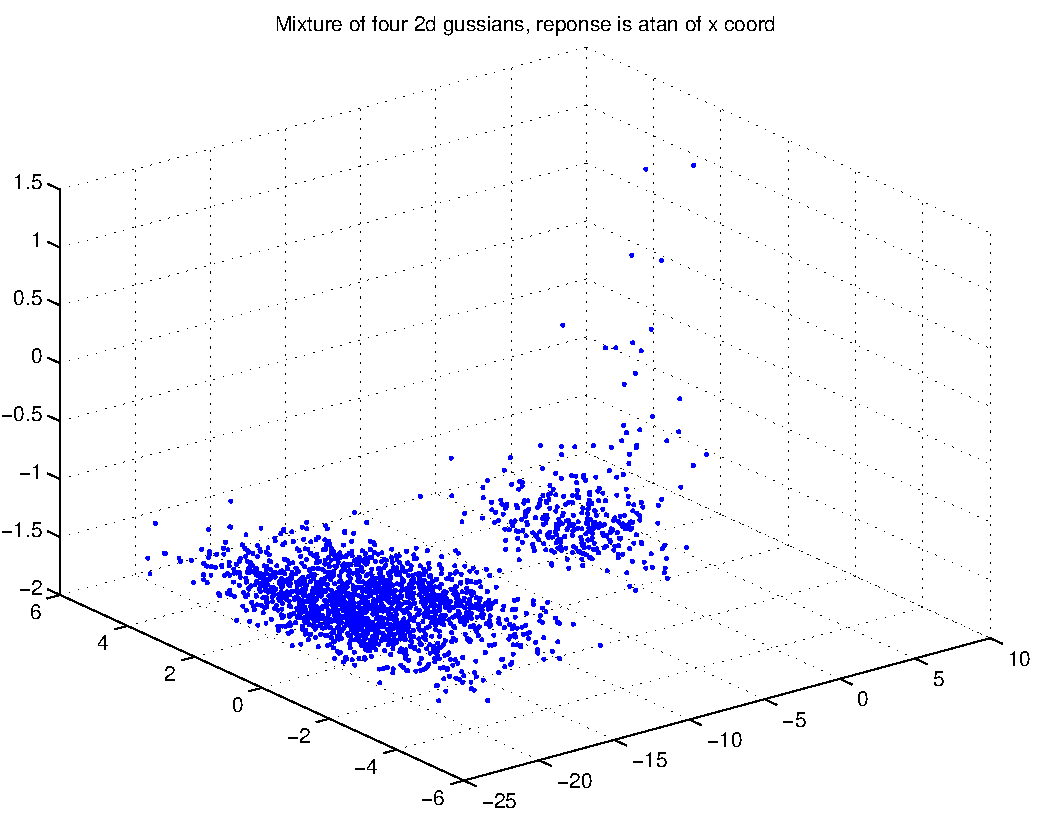
\includegraphics[width=10.0cm,height=10.0cm]{AtanDataSet.pdf}

\subsubsection{3 x 1 Linear Regression}
Sample size = 4000

Number of features = 3

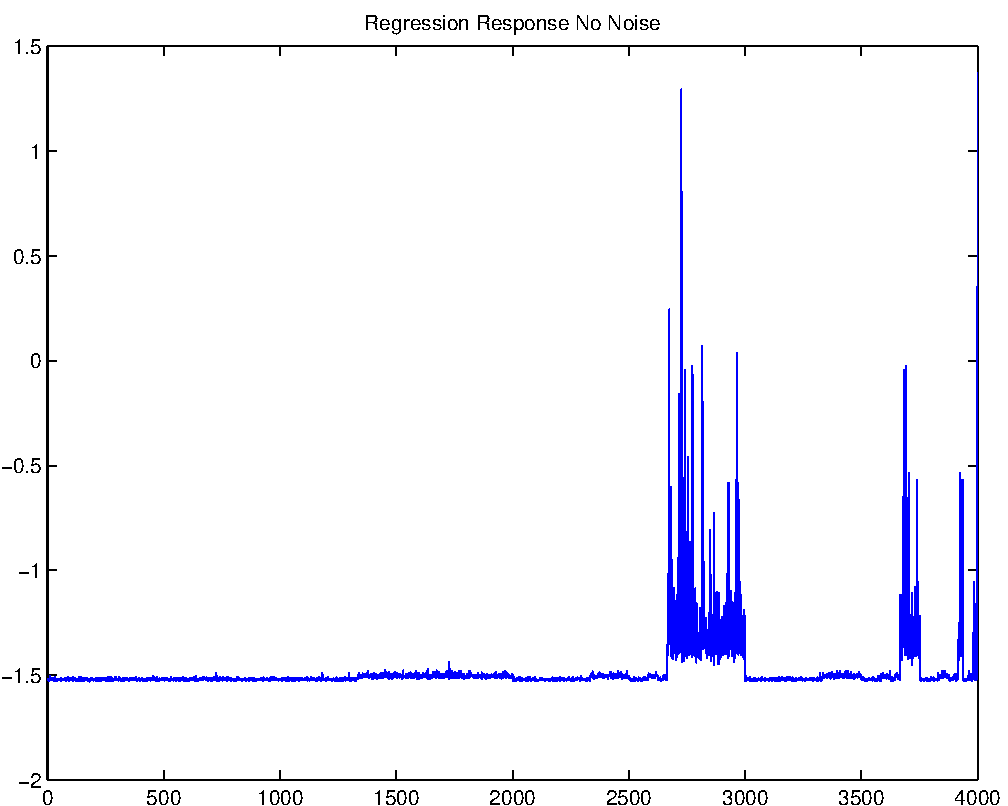
\includegraphics[width=10.0cm,height=10.0cm]{AtanDataSet_regression_response_no_noise.pdf}

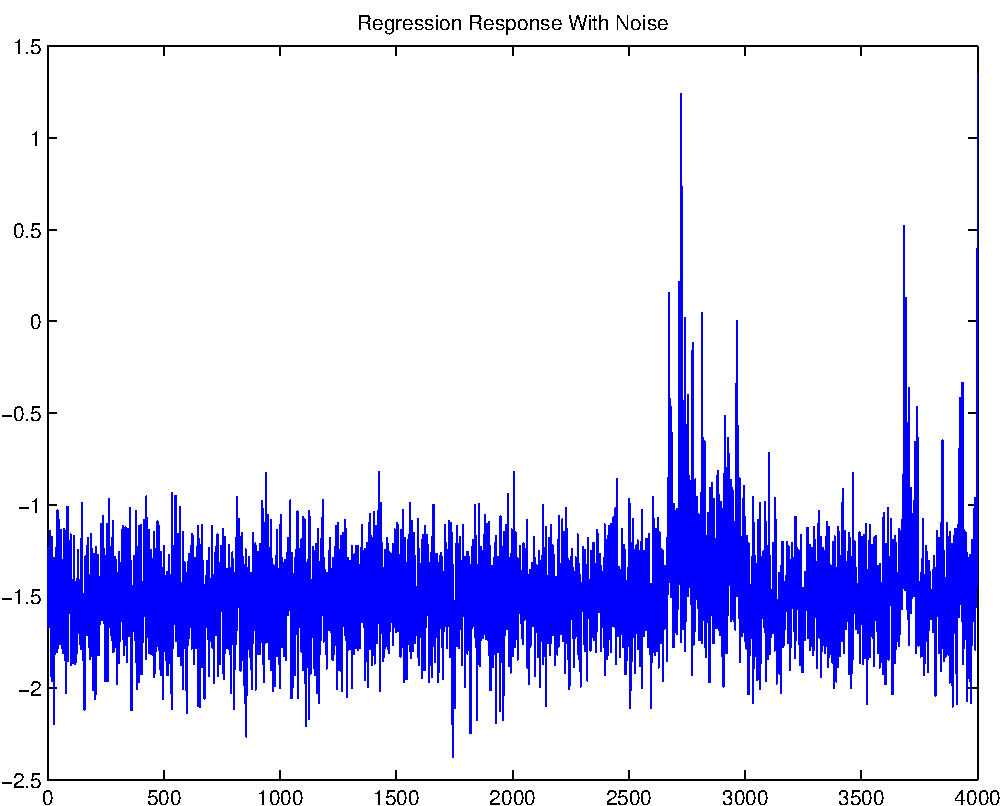
\includegraphics[width=10.0cm,height=10.0cm]{AtanDataSet_regression_response_with_noise.pdf}

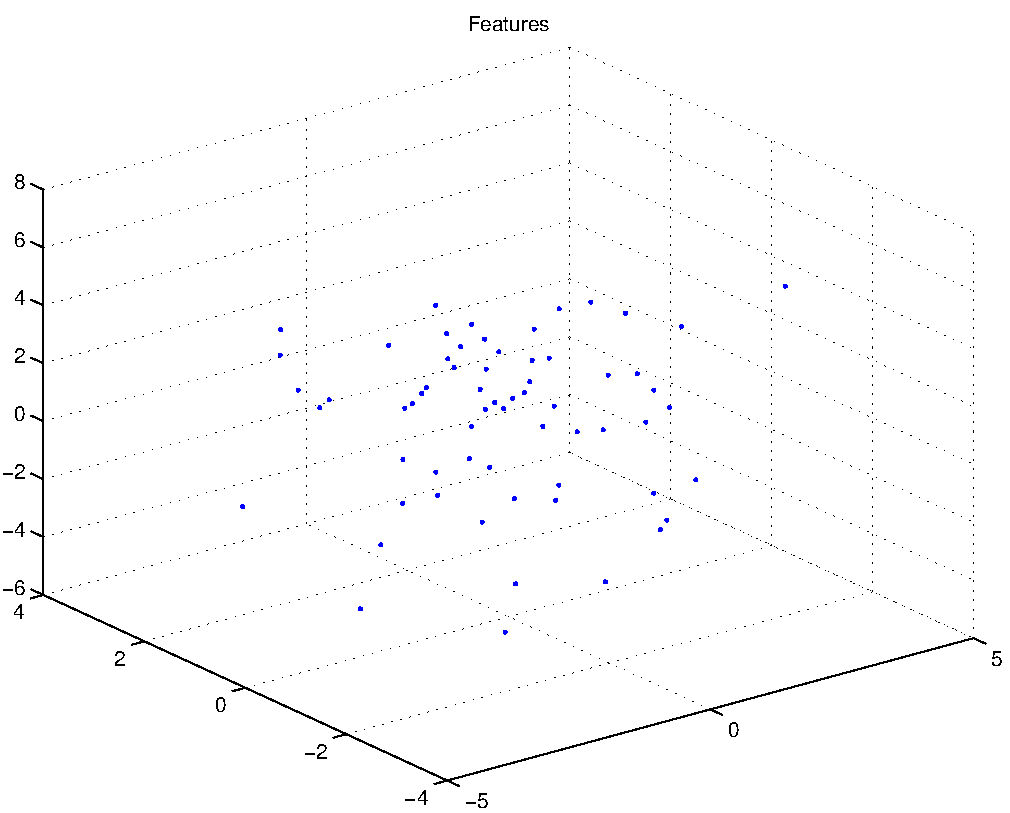
\includegraphics[width=10.0cm,height=10.0cm]{regression_features.pdf}

Response
-1.43552
-1.65332
-1.34694
1.63455
-1.31001
-1.32669
-1.11354
1.60799
-1.30867
-1.11836
-1.19182
1.53814
-1.74267
-1.4887
-1.2319
0.913099
-1.17337
-1.3615
-1.74173
1.25956
-1.42653
-1.52142
-1.13089
1.00133
-1.48063
-2.17849
-1.16418
1.36331
-1.44933
-1.74032
-0.898769
1.58103
-1.80578
-1.77362
-1.47229
1.61843
-1.26116
-1.48441
-1.1142
1.06425
-1.16741
-1.36789
-0.842931
1.57909
-1.22702
-1.75337
-1.21642
1.20119
-1.51376
-1.04674
-0.516367
1.66421
-1.55851
-1.74583
-1.26007
1.16449
-1.45409
-1.11897
-1.44491
1.18917
-1.48791
-1.7527
-1.21173
1.2542
-1.81247
-1.28889
-1.37142
1.01107
-1.52188
-1.45182
0.79127
1.82995
-1.74431
-1.22189
-1.52602
0.941949
-1.60614
-2.00829
-0.927948
1.26966
-1.43887
-1.51106
-1.4328
1.83247
-1.34075
-0.986567
-1.19438
1.41778
-1.84965
-1.54119
-1.26316
1.49249
-1.38349
-1.50859
-1.15836
1.28837
-1.38167
-1.21356
-0.946853
0.988398
-1.83178
-1.52151
-1.49541
0.892706
-1.70894
-1.82978
-1.33013
0.794108
-1.60987
-1.60731
-1.57157
1.45226
-1.17373
-1.35189
-1.42221
1.29555
-1.81609
-1.40777
-1.73273
1.2251
-1.66639
-1.59861
-1.42308
1.18515
-1.80223
-1.53814
-1.4656
1.41928
-1.41161
-1.22493
-1.44136
1.26134
-1.69675
-1.64002
-1.19093
1.38738
-1.58146
-1.76111
-1.58838
1.3235
-1.65586
-1.42459
-0.00472027
1.18185
-1.80572
-1.183
-1.65042
1.36636
-1.63146
-1.76271
-1.69664
1.26997
-1.47856
-1.70092
-1.03689
1.28387
-1.6767
-1.467
-1.8563
1.17119
-1.38447
-1.28502
-1.01355
1.45653
-1.68274
-1.57542
-1.08542
1.65863
-1.72252
-1.49437
-1.27642
1.15995
-1.37389
-1.1725
-1.0108
1.29321
-1.63172
-1.76223
-1.27265
1.48324
-1.49082
-1.57162
-1.59606
1.2776
-1.48967
-1.81896
-1.07794
1.05237
-1.54938
-1.42201
-1.22841
1.68659
-1.73351
-1.3708
-1.29318
1.4147
-2.01183
-1.39504
-1.35213
1.22438
-1.26754
-1.34162
-1.78065
1.14255
-1.35405
-1.39869
-1.92509
1.25095
-1.46303
-1.20273
-1.29651
1.60032
-1.61584
-1.72511
-1.13566
1.3707
-1.5071
-1.78556
-1.34367
1.3897
-1.81823
-1.42274
-1.47192
1.28301
-1.45087
-1.38286
-1.53051
1.13408
-1.54384
-1.08745
-1.32364
1.32376
-1.39085
-1.14982
-1.31452
1.26799
-1.51282
-1.41844
-1.12263
1.83525
-1.48409
-1.5239
-1.52929
1.08733
-1.32395
-1.71755
-0.990348
1.4424
-1.96847
-1.50434
-1.30476
1.42286
-1.42067
-1.32192
0.550813
1.40646
-1.33439
-1.56199
-1.17536
0.864147
-1.96068
-1.4597
-0.755171
1.54249
-1.65916
-1.17167
-1.12903
1.64554
-1.56921
-1.62086
-1.35427
1.52567
-1.62576
-1.41989
-1.45787
1.43484
-1.19546
-1.72547
-0.990759
1.0298
-1.34795
-1.44592
-0.914168
1.02524
-1.64393
-1.58725
-1.55827
1.23106
-1.51693
-1.35035
-1.17769
0.915189
-1.43926
-1.29073
-1.3819
1.32266
-1.42481
-1.47553
-1.81316
0.844757
-1.38002
-1.44367
-1.42992
1.26224
-1.67201
-1.58187
-0.726114
1.0644
-1.45837
-1.73315
-1.16958
1.34314
-1.64127
-1.31548
-1.40839
1.16302
-1.57812
-1.48256
-0.871813
1.79692
-1.50845
-1.50788
-1.58294
1.37953
-1.11952
-1.57154
-1.36494
1.05145
-1.42231
-1.60203
-1.50736
1.12369
-1.41692
-1.54685
-0.938083
1.18251
-1.41215
-1.17824
-1.28291
1.63951
-1.4231
-1.16474
-1.69378
1.49125
-1.13409
-1.6077
-1.4226
1.15838
-1.41251
-1.42355
-1.59334
1.35085
-1.45572
-1.21529
0.924242
1.87339
-1.60032
-1.46416
-1.21568
1.40923
-2.12899
-1.43641
-1.81416
1.23887
-1.45565
-1.66331
-1.27462
1.23203
-1.60972
-1.66223
-0.85161
1.4205
-1.5146
-1.67519
-1.30822
1.42028
-1.58508
-1.71743
-1.69102
1.74715
-1.86501
-1.3693
-1.91968
0.517286
-1.59702
-1.60787
-1.06188
1.10211
-1.24645
-1.34825
-1.19063
0.869887
-1.78238
-1.1034
-1.57657
1.41699
-1.62095
-1.86296
-1.46775
1.3811
-1.11822
-1.61015
-1.46974
0.707978
-1.67638
-1.53769
-1.52783
1.22953
-1.58524
-1.45799
-1.25548
1.51161
-1.49616
-1.42301
-1.21499
1.61991
-1.07524
-1.32129
-1.16075
1.26838
-1.50049
-1.81255
-1.28174
1.65834
-0.947219
-1.55389
-0.393121
1.20907
-1.26519
-1.4284
-1.28678
1.54939
-1.17649
-1.36522
-1.00122
1.187
-1.80313
-1.67625
-1.31742
1.43639
-1.57168
-1.59182
-1.57977
1.31518
-1.2478
-1.3805
-1.60573
1.55375
-1.31626
-1.43072
-0.893431
1.60582
-1.83775
-1.63632
-1.40875
0.631203
-1.14932
-1.21042
-0.941569
1.2841
-1.90204
-1.54486
-1.79054
0.958373
-1.25065
-1.74093
-1.68728
1.14819
-1.53761
-1.18547
-1.25315
1.15919
-1.09149
-1.15332
-1.41851
1.1055
-1.38931
-1.09544
-1.25147
1.09594
-1.23123
-1.6966
-1.55346
1.56918
-1.72354
-1.5081
-1.24919
1.53868
-1.93318
-1.45285
-1.50966
1.15081
-1.49739
-1.50865
-1.20161
1.37173
-2.04972
-1.31796
-1.46341
1.30032
-1.22546
-1.26497
-1.53775
1.3476
-1.77884
-1.5589
-1.06546
1.38504
-1.85013
-1.40179
-1.40932
1.2646
-1.82399
-1.61159
-1.22578
0.838664
-1.77233
-1.51128
-1.1811
1.42781
-1.27352
-1.78131
-1.22087
1.1255
-1.86235
-1.74212
-1.55164
1.43275
-1.39123
-1.49343
-1.28961
0.530514
-1.40378
-1.47806
-0.779208
1.23532
-2.11964
-1.33014
-1.30172
1.32035
-1.42387
-1.28457
-1.16102
1.23666
-1.48918
-1.42684
-1.29773
1.4543
-1.46831
-0.942043
-1.13561
1.11637
-1.74748
-1.52077
-1.40002
1.3954
-1.61655
-1.36626
-1.02904
1.45871
-1.46402
-1.15641
-1.73395
0.887599
-1.72939
-1.44022
-1.28608
1.2424
-1.00707
-1.53023
-1.30264
1.39798
-1.87124
-1.65679
-1.27043
0.961681
-1.55916
-1.55673
-1.56173
1.10799
-2.00341
-1.33023
-0.975728
1.13031
-1.51092
-1.53396
-1.5599
1.20679
-1.30748
-1.46046
-1.27572
0.997128
-1.4907
-1.58094
-1.3549
1.42584
-1.84984
-2.11597
-1.59769
1.36203
-1.7327
-1.522
-1.31399
0.702557
-1.76678
-1.30453
-1.24362
1.0142
-1.71977
-1.23386
-1.23921
1.25377
-1.41922
-1.43477
-1.58946
0.629341
-1.22348
-1.48095
-1.21724
1.09886
-1.17904
-1.25755
-0.883546
1.70165
-1.52224
-1.33157
-1.16184
1.3177
-1.31785
-1.84803
-1.5681
1.17914
-1.29306
-1.67954
-1.19167
1.18228
-1.46026
-1.75827
-1.22567
1.50865
-1.77822
-1.26346
-1.09796
1.45653
-1.51331
-1.73279
-1.33343
1.79878
-2.09322
-1.25
-1.19227
1.26701
-1.1778
-2.05773
0.104317
1.40765
-1.42467
-1.54097
-1.27635
1.32648
-1.44069
-1.69503
-1.23664
0.901768
-1.10883
-1.28177
-1.57139
1.5022
-1.31132
-1.60873
-1.41714
1.2199
-1.4509
-1.75292
-1.95856
1.0365
-1.82131
-1.82553
-1.59199
1.43874
-1.62736
-1.63963
-1.16421
1.58065
-1.45439
-1.38648
-0.40449
1.64315
-1.73839
-1.46808
-1.1359
1.55835
-1.94211
-1.22525
-1.32446
1.16382
-1.42572
-1.70353
-1.19575
1.20194
-1.40374
-1.55155
-1.57557
1.20367
-1.41851
-1.3815
-1.20414
1.77177
-1.78838
-1.40411
-1.5265
1.11244
-1.72271
-1.37814
-1.79168
0.996818
-1.41187
-1.66985
-1.19115
0.870489
-1.49715
-1.29731
-1.074
1.32216
-1.51612
-1.40047
-1.4164
1.13499
-1.28488
-1.52967
-0.869423
0.957591
-1.52664
-1.40866
-1.08177
1.34623
-1.53167
-1.58729
-1.52782
0.953952
-1.32851
-1.73224
-1.32752
1.40065
-1.27789
-1.56872
-1.40534
1.36927
-1.45279
-1.37832
-0.829798
1.36265
-1.44128
-1.90925
-1.2049
1.45285
-1.53051
-1.83507
-1.35468
0.842739
-1.33533
-1.63183
-1.30457
0.933536
-1.17893
-1.6256
-1.45316
1.43971
-1.54197
-1.64769
-1.15821
1.14536
-1.78171
-1.50818
-1.51039
1.12892
-1.74587
-1.42221
-1.63791
1.45311
-1.31917
-1.76859
-1.25423
1.55879
-1.80935
-1.49046
-1.3483
1.32073
-2.02685
-1.4646
-1.48083
1.06226
-1.64982
-1.69985
-1.13269
0.988217
-1.52719
-1.28159
-1.32924
0.900535
-1.41919
-1.79405
-1.97331
0.891275
-1.4114
-1.62732
-1.12148
1.00871
-1.1862
-1.18652
-1.17239
0.984033
-1.59187
-1.57567
-0.887426
0.913413
-1.34019
-1.38322
-1.41085
1.45026
-1.08851
-1.50231
-1.40954
1.3028
-1.47519
-1.3124
-1.6325
1.30078
-1.5606
-1.88941
-1.36361
1.34806
-1.17603
-1.45007
-1.26207
1.36514
-1.15581
-1.3013
-1.37823
0.854294
-1.45051
-1.27278
-1.51999
1.06247
-1.9881
-1.31135
-1.33787
1.26764
-2.09005
-1.57535
-1.69086
1.49221
-1.62568
-1.58122
-2.11495
1.05112
-1.79794
-1.40905
-1.13273
1.21764
-1.53298
-1.74
-1.57808
1.2591
-1.48023
-1.29278
-1.54506
1.51811
-1.65307
-1.80763
-1.28372
1.41998
-1.67563
-1.34444
-1.3945
0.990999
-1.69645
-1.50922
-1.73102
0.649954
-2.00709
-1.13472
-1.36298
1.03089
-1.35009
-1.40371
-1.49493
1.08512
-1.65476
-1.31239
-1.4041
1.36913
-1.56454
-1.18285
-1.62917
1.48575
-1.47083
-1.21774
-1.61449
0.784062
-1.80426
-1.61937
-1.09376
1.56561
-1.80927
-1.77184
-0.933158
1.29401
-1.59815
-1.36255
-1.53251
1.3864
-1.29708
-1.20456
-1.6876
1.2538
-1.54663
-1.47836
-1.57883
1.09823
-1.39663
-0.965235
-1.4778
1.49852
-1.57627
-1.43146
-0.880367
1.072
-1.88327
-1.70485
-1.85328
0.917221
-1.7535
-1.58603
-1.13375
1.3587
-1.09686
-1.38769
-1.1769
1.15049
-0.828916
-1.72199
-1.05213
1.48281
-1.56389
-1.54546
-0.953806
1.02275
-1.51661
-1.44408
-1.62864
1.34533
-1.39661
-1.2141
-1.04045
1.60976
-1.82449
-1.65803
-1.12546
1.34974
-1.90395
-1.0839
-1.51704
0.993523
-1.68107
-1.31605
-1.59867
1.5137
-1.68366
-1.37655
-1.76933
1.05851
-1.59164
-1.70848
-1.16443
0.90223
-1.55587
-1.63557
-0.964266
1.41276
-1.27725
-1.43228
-1.33952
1.34257
-1.13685
-1.24748
-1.57251
1.29596
-1.4861
-1.43519
-1.31176
1.20603
-1.3489
-1.38099
-1.69086
1.47556
-1.60439
-1.19144
-0.996893
1.09997
-1.99489
-1.64785
-0.757206
1.15242
-1.61037
-1.58901
-1.05797
1.45388
-1.78133
-1.3264
-1.44902
1.24719
-1.35309
-1.46263
-1.11213
1.54658
-1.82517
-1.44712
-1.37072
1.51754
-1.29549
-1.67028
-1.15627
1.3926
-1.54915
-1.53313
-1.47729
1.64913
-1.54914
-1.45906
-1.42848
1.12305
-1.38956
-1.56177
-0.198771
1.35245
-1.25293
-1.44384
-1.04613
1.54718
-1.51634
-1.46499
-1.41076
1.83595
-1.5747
-1.51057
-1.36883
1.45595
-2.06037
-1.58951
-1.70015
1.3673
-1.44854
-1.99152
-1.57884
1.1318
-1.72944
-1.41399
-1.40602
1.23882
-1.3766
-1.39143
-1.25919
1.26083
-1.94204
-1.32676
-1.16307
0.795042
-1.39299
-1.25233
-1.00285
1.7101
-1.69255
-1.35424
-0.151269
0.888202
-1.83958
-1.51184
-1.24383
1.31646
-1.50572
-1.6556
-1.18055
0.149082
-1.61579
-1.63796
-1.46964
1.34113
-1.39091
-1.44884
-1.05975
0.956219
-1.50302
-1.44568
-1.5105
1.17677
-1.28766
-1.34534
-1.6099
1.75487
-1.89807
-1.32885
-1.0991
1.06537
-1.07614
-1.76349
-1.04102
0.927253
-1.52729
-1.29652
-1.84233
1.15792
-1.55075
-1.5015
-1.70575
1.01956
-1.32725
-1.87714
-1.32891
1.02495
-1.5468
-1.28033
-1.45311
0.706457
-1.01137
-1.52848
1.35524
1.45072
-1.78957
-1.57348
-1.5818
1.28375
-1.48805
-1.85365
-0.918847
1.29062
-1.4173
-1.55463
-1.45234
0.982482
-1.37525
-1.21006
-1.10881
1.37387
-1.65938
-1.24384
-1.32109
0.941716
-1.38319
-1.45806
-0.725707
1.42993
-1.34944
-1.789
-0.89722
1.26453
-1.65057
-1.29316
-1.01631
0.843069
-1.77393
-1.12643
-1.64976
0.471991
-1.74227
-2.05478
-1.34963
1.60167
-1.58894
-1.53253
-0.902821
1.09583
-1.46706
-1.3278
-0.794849
1.44436
-1.17738
-1.57207
-0.855811
1.53071
-1.59587
-1.20491
-0.692908
1.34416
-1.33047
-1.39881
-1.03998
1.17962
-1.53013
-1.26056
-0.87301
1.47912
-1.61689
-1.5659
-0.0189481
1.57686
-1.73653
-1.70975
-1.52137
0.958995
-1.37309
-1.47572
-1.60143
1.13787
-1.45241
-1.51066
-1.25053
1.31787
-1.51421
-1.45813
-1.39413
1.56198
-1.17799
-1.32741
-1.01643
1.52458
-1.6088
-1.32516
-1.22283
1.18007
-1.65848
-1.81611
-1.28787
1.26401
-1.77851
-1.71184
-1.19257
0.739738
-1.29586
-1.38761
-1.73685
0.607651
-1.45343
-1.4378
-1.43075
1.65111
-1.52468
-1.34676
-1.17747
1.01096
-1.16715
-1.27312
-0.62876
1.55742
-2.01167
-1.40521
-1.40754
1.29995
-1.5343
-1.44301
-0.743094
1.04009
-1.63445
-1.61155
-1.57757
1.31999
-1.25432
-1.64604
-0.962302
1.0044
-1.67504
-1.16131
-1.51728
0.909461
-2.00751
-1.48649
-0.934497
1.66234
-1.45731
-1.43551
-0.836987
1.28463
-1.65994
-1.62712
-1.18555
1.24161
-1.59701
-1.63901
-1.33181
1.09664
-1.08262
-1.71662
-1.24959
1.70558
-1.3218
-1.68621
-1.22091
0.867013
-1.49973
-1.34807
-1.6481
1.30319
-1.39306
-1.53833
-1.60067
1.23608
-1.5643
-1.70231
-1.22595
1.04755
-1.5323
-1.29499
-1.41092
1.34497
-1.6144
-1.62753
-1.61171
1.60458
-1.99888
-1.58491
-1.07369
1.46548
-1.5086
-1.2533
-1.25628
1.58265
-1.44942
-1.78133
-0.759159
1.22329
-1.72435
-1.27765
-1.08253
1.04864
-1.75334
-1.21265
-1.31989
1.15293
-1.67736
-1.66962
-1.38405
1.30124
-1.78219
-1.22595
-1.56193
1.06754
-1.57686
-1.48107
-1.2682
1.37631
-1.67096
-1.53525
-1.49757
1.0373
-1.44558
-1.31851
-1.26794
1.19762
-1.27388
-1.23294
-1.32834
1.70402
-1.64674
-1.37486
-1.16418
1.55884
-1.39593
-1.30529
-1.23814
1.3813
-1.53567
-1.68483
-1.2501
0.853405
-1.97922
-1.25296
-1.74374
0.981793
-1.54733
-1.60873
-1.67384
1.37707
-1.54967
-1.22912
-1.22076
1.36706
-1.99728
-1.67361
-0.643781
1.40379
-1.65102
-1.10157
-1.32177
1.52499
-1.55692
-1.33829
-1.59539
1.79615
-1.19585
-1.1906
-1.5742
0.890216
-1.57167
-1.33074
-1.75858
1.38985
-1.344
-1.60987
-0.548955
1.10217
-1.21833
-1.41833
-1.34791
1.27065
-1.06748
-1.80375
-1.63496
1.62641
-1.69577
-1.38534
-0.980113
1.27468
-1.37163
-1.10475
-1.19894
1.4821
-1.75407
-1.16
-1.37114
1.27152
-1.38203
-1.46056
-1.17659
1.95782
-1.33239
-1.55837
-1.5053
1.25311
-1.73839
-1.22211
-1.79505
1.35459
-0.998732
-1.34332
-0.965253
1.51541
-1.71307
-1.54232
-1.10804
1.06252
-1.38351
-1.85139
-1.22951
1.45413
-1.46117
-1.48859
-1.67633
1.43499
-1.77654
-1.72947
-1.33052
0.99605
-1.28621
-1.59186
-1.17409
1.4496
-1.65561
-1.79461
-1.39732
1.44517
-1.72536
-1.51525
-1.05125
1.01601
-1.48269
-1.43418
-1.45814
1.05316
-1.34019
-1.30581
-1.4213
1.59978
-1.64514
-1.69441
-1.40594
1.53171
-1.45846
-1.63588
-0.972956
1.36537
-1.30978
-1.27713
-1.33632
1.41615
-1.77273
-1.4197
-1.15399
1.6166
-1.52642
-1.48744
-1.14478
1.25186
-1.15575
-1.3333
-1.14438
1.22297
-1.2943
-1.54446
-1.38047
1.14919
-1.42902
-1.09292
-1.35814
1.62511
-1.24821
-1.60113
-0.965999
1.25648
-1.70956
-1.27772
-1.3161
1.00241
-1.63013
-1.51296
-0.794868
1.44451
-1.56066
-1.83135
-1.41671
1.25832
-1.15786
-1.35541
-0.906377
1.21782
-1.66198
-1.59338
-1.24445
1.80095
-1.43521
-1.4995
-1.6066
1.37282
-1.98101
-1.36932
-1.25045
0.815227
-1.56476
-1.17284
-1.28587
1.19867
-1.326
-1.54907
-1.24441
0.873392
-1.38398
-1.61206
-1.34271
1.43735
-1.78014
-1.33533
-0.852333
1.2524
-1.18613
-1.4046
-0.277514
1.51025
-1.80578
-0.989948
-1.14826
1.43988
-1.59427
-1.58913
-1.62315
1.09516
-1.12212
-1.28713
-1.22016
1.59785
-1.4267
-1.47968
-1.62046
1.36712
-1.58513
-1.6326
-1.42863
1.68723
-1.3427
-1.28784
-1.26172
1.23532
-1.7624
-1.695
-1.37896
1.2837
-1.69271
-1.6977
-1.55387
1.13209
-1.45425
-1.49021
-1.57706
1.34396
-1.85715
-1.08163
-1.18707
1.03944
-1.61958
-1.23599
-1.44436
1.39172
-1.73604
-1.39225
-1.56032
0.884545
-1.33615
-1.54975
-1.53976
1.21282
-1.28758
-1.94216
-1.10747
1.18871
-1.59923
-1.47304
-1.62536
0.890862
-1.18601
-1.48008
-1.38066
1.46578
-1.92143
-1.12339
-1.32026
1.15386
-1.64343
-1.45887
-1.54048
1.25852
-1.58124
-1.47417
-0.761334
1.42118
-1.52569
-1.21773
-1.53051
0.750032
-1.36642
-1.34046
-1.0901
1.34531
-1.98305
-1.73487
-1.055
1.42712
-1.45975
-1.64251
-1.45108
1.02316
-1.54289
-1.59964
-1.26509
1.54703
-1.63114
-1.43306
-1.84291
1.10402
-1.80312
-1.59776
-1.53507
1.82425
-1.39691
-1.39031
-1.46883
1.47324
-1.69796
-1.88381
-1.21691
0.945537
-1.75171
-1.26834
-1.52367
1.5424
-1.29586
-1.60082
-1.17725
1.58504
-1.50042
-1.63766
-0.970549
0.940771
-1.64681
-1.32433
-1.38536
0.832426
-1.75375
-1.48338
-1.23531
1.61589
-1.60412
-1.33141
-0.855768
1.25987
-1.6946
-1.25532
-0.840739
1.12786
-1.71795
-1.7616
-1.39543
0.927162
-1.4505
-1.51539
-1.21247
1.53806
-1.70523
-1.61014
-0.767665
1.37643
-1.13508
-1.36965
-1.35446
1.24058
-1.48951
-1.21062
-0.912178
1.65179
-1.59933
-1.24899
-1.59977
1.48044
-1.28944
-1.33587
-0.98171
1.61484
-1.70127
-1.17005
-1.03656
1.81585
-1.57627
-1.29855
-1.00769
1.01341
-1.70793
-1.67272
-0.992057
1.16607
-1.45671
-1.63451
-1.38905
1.62911
-1.97575
-2.38857
-1.23241
1.13311
-1.79437
-1.99343
-1.33357
1.35187
-1.56295
-1.73592
-1.46615
1.13085
-2.13775
-1.99522
-0.788877
1.70792
-1.56738
-1.49314
-1.24351
1.05461
-1.41459
-1.11516
-1.51074
1.31959
-1.72092
-1.73727
-1.23992
1.11051
-1.38196
-1.63445
-1.3775
1.44832
-1.18224
-1.1736
-0.741255
1.54556
-1.66755
-1.58256
-1.20225
1.25166
-1.86474
-1.59723
-1.32358
1.48881
-1.22076
-1.1097
-1.05655
1.44772
-1.53789
-1.44508
-1.36954
1.33833
-1.3848
-1.44759
-1.19786
1.54909
-2.00204
-1.30348
-1.25103
1.31473
-1.68564
-1.48531
-1.39886
1.25045
-1.8422
-1.26181
-1.45732
1.0036
-1.38771
-1.78455
-1.07357
1.32848
-1.4575
-1.65373
-1.66419
1.42228
-1.65857
-1.88334
-2.13879
1.25201
-1.58145
-1.36322
-1.49507
1.55792
-1.36078
-1.66793
-1.14492
1.48165
-1.6716
-1.18146
-1.11945
1.63104
-1.67253
-1.6115
-1.05166
1.34822
-1.73129
-1.0111
-1.61694
0.8213
-1.28843
-1.17004
-1.3721
0.937359
-1.70131
-1.71977
-1.47521
0.517064
-1.35468
-1.32109
-1.56816
1.17077
-1.49881
-1.4051
-1.33144
1.86572
-1.88134
-1.53283
-1.10555
1.35905
-1.89895
-1.72922
-1.02172
1.65947
-1.56948
-1.42139
-1.39195
0.97565
-1.28643
-1.41556
-1.19024
1.37025
-1.37004
-1.24711
-1.15193
1.52821
-1.51576
-1.45085
-0.857714
1.85126
-1.59305
-1.4264
-1.0648
1.7132
-1.53963
-1.35794
-1.51944
1.28686
-1.50595
-1.10162
-1.12146
1.19977
-1.46649
-1.72733
-1.00905
1.42605
-1.11406
-1.80834
-1.33421
1.60743
-1.2458
-1.73975
-1.69448
0.833977
-2.03441
-1.58549
-1.39772
1.26691
-1.64054
-1.34193
-1.29485
0.961858
-1.38556
-1.6351
-1.55977
1.46952
-1.63701
-1.66309
-1.41981
1.5502
-1.36313
-1.6942
-1.25279
1.45613
-1.39232
-1.6875
-1.371
1.35169
-2.23055
-1.17134
-1.51405
1.1525
-1.73246
-1.39509
-1.4091
1.16947
-1.37666
-1.27964
-1.52551
1.41144
-1.71435
-1.6345
-1.6053
0.84528
-2.15202
-1.46961
-1.241
1.65344
-1.33342
-1.25981
-0.995231
1.72883
-1.39992
-1.61836
-1.21975
1.39428
-2.1858
-1.83372
-1.52347
1.45615
-1.28752
-1.15754
-1.85983
1.21346
-1.25914
-1.72838
-1.62808
0.720734
-1.28177
-1.30821
-0.936625
1.42469
-1.51817
-1.31022
-1.09785
1.35732
-1.6945
-1.39903
-1.46254
1.11198
-0.958298
-1.59527
-1.09153
1.08066
-1.4346
-1.72895
-1.67965
1.08589
-1.51012
-1.40956
-1.22752
0.837754
-1.32553
-1.32942
-1.34588
1.55208
-1.47298
-1.45183
-1.06499
1.03747
-1.28319
-1.78518
-1.22359
1.36162
-0.806513
-1.47596
0.115289
1.40725
-1.77675
-1.36937
-1.43122
0.962254
-1.1514
-1.32928
-1.28619
1.30028
-1.73625
-1.31793
-1.02882
1.20045
-1.66123
-1.81708
-1.12856
1.26575
-1.5434
-1.46782
-1.2214
1.44351
-1.29525
-1.58187
-1.30771
1.5724
-1.58047
-1.42189
-1.1432
1.33513
-1.5562
-1.63629
-1.19397
1.42993
-1.46392
-1.72016
-1.5619
0.411193
-1.75072
-1.27183
-0.897723
1.38714
-1.42868
-1.42676
-1.10407
1.49564
-1.31464
-1.59417
-1.33001
1.10488
-1.45328
-1.60405
-1.48354
1.53628
-1.70381
-1.06672
-1.24833
0.925871
-1.42693
-1.72299
-1.42274
1.08813
-1.49101
-1.33702
-0.0188888
0.975882
-1.4261
-1.75732
-1.36629
1.54653
-1.54535
-1.3609
-1.66162
1.03166
-1.54277
-1.32811
-0.842914
1.35848
-1.51616
-1.56343
-1.54204
1.32884
-1.40869
-1.42591
-1.21088
1.65679
-1.30082
-1.2468
-1.10273
0.94389
-1.78301
-1.79195
-1.20831
1.32076
-1.36318
-1.57799
-0.99046
1.40824
-1.36554
-1.67413
-1.37959
1.28595
-1.50506
-1.81583
-1.64623
1.56971
-1.63557
-1.67231
-1.39712
0.860331
-1.99548
-1.28347
-1.34749
1.58124
-1.57234
-1.38963
-0.743862
1.42545
-1.28007
-1.63115
-1.11378
1.4849
-1.3036
-1.84687
-0.671186
1.42519
-1.31646
-1.43596
-0.73169
1.6937
-1.47358
-1.49304
-1.25845
0.845688
-1.64969
-1.51882
-0.951301
0.720439
-1.68362
-1.39954
-1.14584
1.27567
-1.67246
-1.3886
-1.21717
1.28514
-1.44128
-1.45252
-1.19002
1.28501
-1.4007
-1.47662
-0.983201
1.37682
-1.52724
-1.7913
-0.89639
1.74648
-1.75754
-1.09496
-1.08521
1.13414
-1.67482
-1.35391
-1.07511
1.4887
-1.21522
-1.64128
-1.45757
1.60343
-1.51711
-1.41531
-1.43475
1.37341
-1.87755
-1.57162
-1.29043
1.04553
-1.39585
-1.54275
-1.43611
1.07045
-1.47511
-1.48604
-1.53622
1.1028
-1.80849
-1.64707
-1.14025
1.32825
-1.18628
-1.75875
-1.04771
1.81525
-1.74571
-1.4333
-1.39849
1.48574
-1.41224
-1.36584
-0.75968
1.28438
-1.56705
-1.54159
-1.04113
1.14091
-1.22225
-1.06124
-1.50518
1.27572
-1.50066
-1.73452
-1.51937
1.26752
-1.37189
-1.68526
-1.06638
0.225685
-1.71759
-1.58729
-1.07205
1.45407
-1.42154
-0.999383
-1.4338
1.54305
-1.64594
-1.44177
-0.878851
1.12398
-1.67653
-1.77491
-1.1279
1.20163
-2.00493
-1.65461
-1.15517
1.52187
-1.33387
-1.96102
-1.04889
1.56543
-1.3032
-1.30471
-1.14726
1.25957
-1.52274
-1.44334
-0.891271
1.59802
-1.62558
-1.3324
-0.936631
1.23364
-1.6245
-1.70102
-1.38641
1.0212
-1.46703
-1.7231
-1.35785
1.5382
-1.53815
-1.49956
-0.618588
1.38872
-1.65561
-1.71305
-1.50329
1.00391
-1.48971
-1.37896
-1.03884
1.75798
-1.72255
-1.74307
-1.56478
1.01988
-1.63657
-1.3036
-1.31861
1.28521
-1.90693
-1.3625
-1.53545
1.00692
-1.99483
-1.41222
-1.38208
1.24665
-1.53899
-1.47374
-1.19392
1.40068
-1.43743
-1.50503
-0.869925
1.68924
-1.24014
-1.22754
-1.23588
1.67758
-1.4751
-1.35842
-1.02371
1.69352
-1.32694
-1.72077
-0.444828
1.36051
-1.51989
-1.30814
-1.20763
1.37622
-1.47543
-1.93872
-0.793686
1.37259
-1.52168
-1.3712
-1.40163
1.31018
-1.43593
-1.44371
-1.47397
1.04591
-1.40645
-1.41395
-1.60142
1.06268
-1.50217
-1.25813
-1.29328
1.06177
-1.48165
-1.68317
-1.20296
1.43585
-1.60243
-1.7137
-1.37819
1.56264
-1.31636
-1.72281
-1.20412
1.51699
-1.67554
-1.51038
-0.28963
1.61787
-1.54978
-1.38524
-1.55312
1.20778
-1.69368
-1.14532
-1.13564
1.72984
-1.39427
-1.58809
-1.09203
1.26863
-1.5189
-1.26736
-0.875482
1.57663
-1.48442
-1.49992
-0.278561
1.36822
-1.42883
-1.37043
-1.56803
1.4686
-1.34758
-1.47458
-1.14394
1.48459
-1.38406
-1.50255
-1.46287
1.04139
-1.58499
-1.42355
-1.45504
1.16256
-1.78384
-1.51273
-1.25787
1.76527
-1.2967
-1.54283
-1.80327
1.07694
-1.42681
-1.54864
-1.33494
1.4842
-1.60767
-1.45465
-1.08371
0.868983
-1.30502
-1.64383
-1.52145
1.71507
-1.33971
-1.11732
-1.19783
1.5509
-1.35019
-1.74313
-1.2623
1.046
-1.44869
-1.10465
-1.23294
1.09504
-1.48358
-1.4966
-1.13679
1.34286
-1.4619
-1.65231
-1.01141
1.30384
-1.48281
-1.07956
-1.29645
1.58001
-1.40428
-1.53857
-1.01858
1.223
-1.49478
-1.63534
-0.876628
0.909543
-1.57648
-1.68094
-1.12579
1.98645
-1.29103
-1.56722
-1.38755
1.51603
-1.70704
-1.58153
-1.24325
1.3922
-1.46171
-1.33317
-1.41364
1.46762
-1.53961
-1.83972
-1.50443
0.951532
-1.72258
-1.67374
-1.29124
0.8868
-1.2823
-1.60866
-0.775647
1.41027
-1.43398
-1.43011
-1.33765
1.3187
-1.576
-1.2256
-1.39143
1.2778
-1.59773
-1.44487
-1.39456
1.2076
-1.26592
-1.92813
-1.37171
1.32573
-1.55163
-1.8379
-1.36012
1.20985
-1.66888
-1.40437
-1.33862
1.43436
-1.72164
-1.52726
-1.03634
1.20326
-0.967953
-1.68141
-1.37347
0.803006
-1.56545
-0.969504
-1.23821
1.43939
-1.7162
-1.68453
-1.87595
1.55756
-1.70441
-1.85265
-1.67653
0.144911
-1.08456
-1.25261
-0.979812
1.20015
-1.72125
-1.70542
-1.06749
1.48301
-1.62863
-1.79964
-1.76035
1.09918
-1.4695
-1.45524
-1.0533
1.37502
-1.44593
-1.65789
-1.57566
1.50938
-1.29485
-1.18552
-1.44324
0.900346
-1.32208
-1.31234
-1.33288
1.36943
-1.54859
-1.65878
-1.20626
1.26415
-1.25049
-1.86887
-1.05614
1.51253
-1.56019
-1.46077
-1.8791
0.621275
-1.02359
-1.06245
-1.38707
1.4343
-1.61064
-1.55115
-1.13498
1.14834
-1.26299
-1.31098
-1.15951
1.38405
-1.6826
-1.30021
-1.42636
1.31444
-1.30451
-1.26294
-1.45056
1.69167
-1.37601
-1.19638
-0.661985
1.75302
-1.46859
-1.41855
-1.51564
0.933088
-1.66896
-1.45241
-1.27717
1.6431
-1.48352
-1.4241
-1.37444
1.19562
-1.82196
-1.67879
-1.57318
1.48831
-1.65986
-1.85315
-1.34981
1.2876
-1.67752
-1.64814
-1.1973
1.39795
-0.978158
-1.79098
-1.5615
1.07543
-1.09622
-1.76169
-1.02274
1.54976
-1.82744
-1.47747
-1.23984
1.65288
-1.27421
-1.12781
-1.17746
1.47541
-1.81179
-1.64775
-0.917757
1.52711
-1.4696
-1.18395
-0.912774
1.56253
-1.88713
-1.45404
-1.25921
1.42417
-1.25631
-1.69968
-1.59674
1.57209
-1.49558
-1.36862
-1.58826
1.57109
-1.43335
-1.48612
-0.742808
1.1932
-1.25571
-1.94585
-1.28027
1.32248
-1.41341
-1.45542
-1.57591
0.716085
-1.57464
-1.66552
-1.06687
1.44749
-1.45852
-1.32527
-1.45806
1.09599
-1.39636
-1.46762
-1.64898
1.28977
-1.17888
-1.52931
-1.33107
1.55767
-1.81297
-1.58376
-1.34906
1.51376
-1.61754
-1.60799
-1.46947
1.40401
-1.21439
-1.5884
-1.44101
1.64617
-1.16573
-1.67268
-0.910667
1.99947
-1.57738
-1.70459
-1.22593
1.34184
-1.67579
-1.77068
-1.50015
0.87867
-1.42508
-1.94027
-0.837575
1.11852
-1.63331
-1.60022
-1.73898
1.42347
-1.72959
-1.74844
-1.28965
1.68266
-1.5975
-1.81058
-1.05558
1.29197
-1.41044
-1.38938
-1.36015
0.949035
-1.6547
-1.67767
-1.44144
1.52942
-1.15157
-1.07625
-1.47252
1.12038
-1.52122
-1.21754
-1.37541
0.728859
-1.40894
-1.55805
-1.15349
1.3857
-1.53946
-1.58366
-1.78871
1.48509
-1.73999
-1.1713
-1.28443
1.04517
-1.51167
-1.34856
-1.05305
1.42314
-1.43501
-1.34218
-1.53726
1.34469
-1.56091
-1.774
-1.32668
1.43302
-1.35932
-1.1974
-1.05324
1.86508
-1.46588
-1.62441
-1.0628
1.62855
-1.00076
-1.39184
-1.37951
0.690586
-1.56198
-1.51226
-0.911203
1.32722
-1.55866
-1.37534
-1.50749
1.11451
-1.41541
-1.90871
-1.9088
1.07342
-1.6284
-1.36272
-0.921003
1.22805
-1.5949
-1.26844
-1.54196
1.14793
-1.69266
-1.78482
-1.67575
1.22036
-1.37033
-1.28393
-1.06224
1.47013
-1.68707
-1.42956
-0.448385
1.29651
-1.7001
-1.10788
-1.36229
1.46573
-1.71703
-1.44286
-1.24495
1.60014
-1.46375
-1.71604
-1.02417
1.08399
-1.80084
-1.52804
-1.3278
1.44351
-1.114
-1.51617
-1.47471
1.19661
-2.01117
-1.34229
-1.33912
1.25572
-1.77855
-1.95409
-1.39715
1.07257
-1.46625
-1.31802
-1.35491
1.2013
-1.7416
-0.936035
-1.2168
0.509334
-1.47436
-1.40984
-1.06823
0.767584
-1.84843
-1.5586
-1.72239
-0.409295
-1.55911
-1.35759
-1.1429
1.23484
-1.28729
-1.65549
-1.6016
1.18175
-1.8507
-1.21993
-1.96951
1.54607
-1.23903
-1.75538
-1.67496
0.888911
-1.69148
-1.43952
-1.00346
1.17342
-1.60588
-1.07557
-1.27771
1.53693
-1.58659
-1.21571
-0.74669
1.03934
-1.29905
-1.21013
-1.16694
1.21403
-1.73419
-1.59657
-1.68729
1.19542
-1.66593
-1.29261
-1.32398
1.24616
-1.79733
-1.12879
-1.18671
1.16378
-1.08639
-1.62791
-1.69685
1.8405
-1.34913
-1.2918
-1.30341
1.61895
-1.36137
-1.83373
-1.64542
0.855809
-1.20102
-1.46913
-1.43842
1.62573
-1.57504
-1.43993
-1.62242
1.25936
-2.00492
-1.33075
-1.00465
1.33485
-1.44561
-1.66957
-2.00943
0.731017
-2.04234
-1.4273
-1.17359
2.17166
-1.61274
-1.16611
-1.3783
1.4286
-1.54993
-1.63766
-1.09316
0.845307
-1.73199
-1.6627
-0.928903
1.39547
-1.19579
-1.54858
-1.5398
1.49479
-1.66058
-1.35909
-1.24213
1.30433
-1.62658
-1.33782
-1.23418
1.35889
-1.4952
-1.67121
-1.17891
0.79076
-1.28268
-1.49203
-1.14156
1.16092
-1.27478
-1.55423
-1.0428
1.74177
-1.09644
-1.35214
-1.11432
1.31371
-1.7203
-1.48888
-1.49078
1.24677
-1.5001
-1.76062
-1.07008
1.58743
-1.43862
-1.26468
-1.55044
1.32665
-0.932734
-1.56587
-1.33471
1.42266
-1.48307
-1.15951
-0.95839
1.31267
-1.64909
-1.80408
-1.52384
1.5407
-1.97022
-1.666
-0.62003
1.60184
-1.63471
-1.64938
-1.45749
1.15651
-1.74862
-1.7736
-1.16475
0.889378
-1.86032
-1.08091
-1.49443
1.3508
-1.61585
-1.34969
-1.72802
1.16163
-1.2274
-1.39104
-1.28534
1.44746
-1.46103
-1.72674
-1.45473
1.45048
-1.7934
-1.2854
-1.04521
1.35272
-1.64828
-1.5517
-0.841673
1.6545
-1.41149
-1.74869
-1.93859
0.882081
-1.62228
-1.2139
-1.4621
0.872829
-1.50392
-1.80974
-1.48705
1.44685
-1.60994
-1.71544
-1.45817
1.13522
-1.4679
-1.26303
-1.23574
1.60967
-1.93583
-1.63026
-0.786505
0.739295
-1.56144
-1.53355
-0.562224
1.03897
-1.60848
-1.747
-0.941882
1.63899
-1.58598
-1.57572
-1.6071
1.07581
-1.51958
-1.75667
-1.16483
0.846323
-1.55733
-1.56163
-0.869886
0.962302
-1.95492
-1.78286
-1.41955
1.64154
-1.80681
-1.53952
-0.982631
1.8694
-2.00164
-1.40099
-1.68991
1.52866
-1.51318
-1.53831
-1.17882
1.02915
-1.5943
-1.35657
-1.27607
1.60438
-1.27287
-1.53448
-0.931843
1.57138
-1.3614
-1.48164
-1.52482
1.14374
-1.65844
-0.96732
-1.28745
1.1621
-1.96531
-1.19482
-0.968242
1.21855
-1.57044
-1.24705
-1.08301
1.27389
-1.50512
-1.3325
-1.02841
1.00096
-1.79293
-1.50607
-0.510396
1.21102
-1.78452
-1.40259
-1.25744
1.6188
-1.82568
-1.5964
-1.4947
0.730721
-1.524
-1.53285
-1.34622
1.37169
-1.65148
-1.68918
-1.46629
0.983824
-1.21206
-1.39672
-1.46114
1.37872
-1.57616
-1.36389
-1.65414
1.21131
-1.39567
-0.945996
-1.29677
1.38985
-1.24859
-1.07391
-1.52962
0.693017
-1.50627
-1.4867
-0.594325
1.2933
-1.73468
-1.7035
-1.26019
1.09744
-1.44908
-1.39684
-1.18352
0.917519
-1.54259
-1.5624
-1.60396
0.728636
-1.52432
-2.0221
-1.18899
1.17369
-1.64687
-1.6387
-1.47127
1.13867
-1.2007
-1.40552
-1.60676
1.30005
-1.58325
-1.75459
-1.60105
1.11286
-1.58671
-1.54368
-1.2272
1.30051
-1.67783
-1.41724
-1.18098
1.46749
-1.51055
-1.4845
0.727492
1.69816
-1.40225
-1.19244
-1.39443
1.02691
-1.23703
-1.69945
-1.00308
1.30577
-1.60094
-1.25438
-1.5471
1.40095
-1.91664
-1.8802
-1.55788
1.32733
-1.77214
-1.74829
-1.27444
1.57594
-1.26041
-1.39616
-1.24376
1.01614
-1.32571
-1.41403
-1.0761
1.31691
-1.50565
-1.60909
-1.33682
0.948391
-1.63195
-1.56457
-1.27868
1.10035
-1.06087
-1.45157
-1.55709
0.905151
-1.24531
-1.3266
-1.12886
1.41443
-1.23471
-1.34063
-1.20652
1.30168
-1.41309
-1.22599
-1.5213
1.59722
-1.56235
-1.44781
-1.15662
1.51274
-1.87574
-1.65065
-1.05028
0.859897
-1.64981
-1.7476
-1.44931
1.30425
-1.79843
-1.51558
-1.77703
1.2196
-1.57175
-1.68031
-1.25913
1.26491
-1.71005
-1.5837
-1.12321
1.1783
-1.66525
-1.3493
-1.23984
1.26507
-1.50918
-1.51002
-1.28047
1.3247
-1.57379
-1.10279
-1.34652
1.49219
-1.47659
-1.11126
-1.36654
1.10276
-1.40308
-1.47416
-1.30495
1.27739
-1.40708
-1.62338
-1.07673
1.1651
-1.79236
-1.73643
-1.63035
1.17759
-1.77332
-1.26752
-1.48129
1.34582
-1.24049
-1.47911
-1.15142
1.23721
-1.82372
-1.34024
-1.14303
1.77816
-1.79257
-1.24172
-0.993658
1.31169
-1.33925
-1.40989
-1.34327
1.21415
-1.44299
-1.30614
-1.53896
1.02005
-1.50926
-1.86283
-1.27491
1.42342
-1.10028
-1.65593
-0.962415
1.771
-1.03745
-1.14666
-1.44773
1.12525
-1.62607
-1.3611
-1.38418
1.37782
-1.16559
-1.39472
-1.23696
0.95032
-1.79011
-1.52005
-1.22987
0.871278
-1.52049
-1.64914
-1.03445
1.64506
-1.26051
-1.71294
-1.50981
1.24331
-1.52647
-1.7334
-0.945245
1.42909
-1.82635
-1.58642
-1.06529
0.929824
-1.46271
-1.57113
0.637841
1.29873
-1.70138
-1.50557
-1.41994
1.29704
-1.89898
-1.58253
-0.920137
1.08317
-1.6044
-1.14001
-1.35281
1.20341
-1.47997
-1.32874
-1.23146
1.57637
-1.43614
-1.72678
-1.52096
1.3108
-1.51509
-1.35294
-1.35013
0.922875
-1.54642
-1.78878
-1.08135
1.13901
-1.65565
-1.75009
-1.2007
0.518467
-1.17535
-1.19611
-0.675877
1.35607
-1.70861
-1.77956
-1.40253
1.37509
-1.99284
-1.34285
-1.58792
0.910945
-1.68068
-1.12775
-1.68666
1.04623
-1.89812
-1.13978
-1.22358
1.35097
-1.63694
-1.34135
-1.08339
1.55394
-1.84319
-1.46191
-1.53063
1.51072
-1.56874
-1.47726
-1.36073
1.25855
-1.31362
-1.74307
-0.812061
1.91718
-1.04219
-1.4932
-0.615298
1.42216
-1.8239
-1.14904
-0.989246
1.52529
-1.31807
-1.13208
-1.05919
1.44597
-1.68772
-1.49388
-0.0482623
1.61847
-1.63388
-1.44713
-1.43126
1.00537
-1.44212
-1.27248
-1.4811
1.35846
-1.26653
-1.92545
-1.02952
1.25757
-1.27134
-1.60996
-1.04384
1.66444
-1.5287
-1.29545
-1.08716
0.873432
-1.36377
-1.32255
-1.4928
0.863001
-1.58027
-1.8402
-1.12309
2.01222
-1.53961
-1.44498
-0.904021
1.45094
-1.31039
-1.22901
-1.45048
1.58942
-1.43374
-1.45383
-1.51734
0.800093
-1.69375
-1.35146
-1.2184
1.25895
-1.65345
-1.57063
-1.12391
1.20889
-1.71994
-1.55798
-1.37164
0.893152
-1.61668
-1.51622
-1.28043
1.60974
-1.31305
-1.80492
-1.08812
0.987249
-1.38408
-1.42394
-1.25601
1.17163
-1.32006
-1.60994
-1.37307
1.40001
-1.17598
-1.64814
-1.03487
1.28108
-1.86466
-1.31404
-1.1236
1.72857
-1.67366
-1.65567
-1.51308
1.04652
-1.454
-1.36364
-1.32094
1.31884
-1.09993
-1.56175
-1.19314
1.52582
-1.34233
-2.06185
-1.21015
1.21626
-1.43767
-1.47011
-0.608774
1.31124
-1.63882
-1.19005
-1.38453
1.61693
-1.83113
-1.29749
-1.23999
1.36922
-1.32239
-1.65195
-1.28324
1.35292
-1.3736
-1.21359
-1.25579
1.10235
-1.72304
-1.55091
-1.47655
1.31003
-1.43898
-1.86562
-1.06562
1.02673
-1.49615
-1.24392
-1.34198
1.17455
-1.16514
-1.4572
-1.1471
1.72038
-1.42675
-1.65324
-1.15723
1.31967
-1.46984
-1.41057
-1.64528
1.44841
-1.64808
-1.32976
-1.42532
1.37283
-1.62842
-1.57013
-1.75536
1.29468
-1.32072
-1.84506
-1.44818
1.26757
-1.61987
-1.65441
-1.7167
1.34082
-1.86687
-1.42971
-1.40892
1.69414
-1.77601
-1.59061
-1.74079
1.21318
-1.28993
-1.05483
-1.589
1.17816
-1.59737
-1.2721
-1.20341
0.803339
-1.80128
-1.21662
-1.39716
1.48531
-1.39551
-1.63291
-1.48707
1.32835
-1.66354
-1.05404
-0.856704
1.17374
-1.8605
-1.29783
-1.18958
1.31542
-1.44456
-1.53257
-0.891857
1.38711
-1.42801
-1.1695
-1.20213
1.25424
-1.08048
-1.35893
-1.43209
0.802148
-1.64769
-2.02526
-1.10123
1.07026
-1.67356
-1.79314
-1.21187
1.22041
-1.63652
-1.58662
-1.47013
1.74687
-1.86305
-1.54566
-1.62824
1.59898
-1.35419
-1.60764
-1.17365
1.28339
-1.76043
-1.69778
-1.2652
1.15097
-1.73051
-1.679
-1.39998
1.4497
-1.13011
-1.75925
-1.52646
1.15345
-1.31935
-1.43575
-1.82377
1.0602
-1.41825
-1.45038
-1.50556
1.31687
-1.62034
-1.78317
-1.19838
1.20814
-1.67642
-1.65774
-1.51706
1.33714
-1.46413
-1.49909
-1.3352
1.79745
-0.960962
-1.60658
-1.27744
1.56031
-1.25058
-1.97627
-1.1134
1.38791
-1.54512
-1.30209
-1.22461
1.43666
-1.5607
-1.67494
-0.900064
1.19258
-1.65107
-1.78568
-1.1409
1.21852
-2.04141
-1.38852
-1.15687
1.5917
-1.19766
-1.55244
-1.11491
0.991035
-1.18089
-1.12183
-1.42025
1.45986
-1.57639
-1.44982
-1.51427
1.38505
-1.44494
-1.28445
-1.41011
1.17965
-1.38251
-1.41799
-0.974877
1.12856
-1.60925
-1.46303
-0.195076
1.31
-1.51879
-1.24331
-1.41792
0.799114
-1.63669
-1.3507
-1.3846
1.27327
-1.57691
-1.2755
-1.11364
1.70673
-1.63413
-1.8581
-1.26843
1.12859
-1.8374
-1.79423
-1.4253
1.43799
-1.44539
-1.5808
-1.70992
1.18506
-1.37748
-1.61602
-1.24198
1.36841
-1.42722
-1.71206
-1.08743
1.34621
-1.8084
-1.03895
0.144039
1.52558
-1.67856
-1.91028
-1.7035
1.32906
-1.85221
-1.72729
-0.85964
1.26143
-1.4051
-1.20684
-1.39497
1.44208
-1.25894
-1.51457
-1.0312
1.2175
-1.51257
-1.70981
-1.2566
0.902687
-1.43131
-1.29671
-1.1185
1.24856
-1.67527
-1.33553
-1.27795
1.3293
-1.43918
-1.60299
-1.21259
1.33281
-1.58295
-1.44827
-1.34041
1.32141
-1.58222
-1.44287
-1.28959
1.55015
-1.69566
-1.58433
-1.35822
1.26587
-1.63929
-1.55036
-1.29471
1.34961
-1.65014
-1.53551
-1.84852
1.38656
-1.80503
-1.64013
-1.54455
1.58008
-1.40936
-1.50203
-0.753443
1.47433
-1.60816
-1.51405
-0.920392
1.61655
-1.17561
-1.69918
-1.54942
1.09851
-1.56744
-1.61966
-0.840121
1.20193
-1.12072
-1.76811
-1.27132
0.734536
-1.7857
-1.3672
-1.2701
1.52443
-0.692136
-1.41013
-1.452
1.34913
-1.46521
-1.4399
-0.850505
1.04651
-1.40681
-1.39893
-1.36351
1.14126
-1.57851
-1.83038
-1.66122
1.08245
-1.71698
-1.70226
-1.1156
1.14028
-1.11441
-1.21041
-1.08195
1.13135
-1.4443
-1.81094
-1.41794
1.41911
-1.32019
-1.50151
-0.959926
0.942485
-1.14084
-1.53395
-1.52315
1.519
-1.37912
-1.35096
-1.16208
1.67621
-1.98972
-1.49341
-1.56046
1.57264
-2.09836
-1.40441
-1.45115
1.23357
-1.37548
-1.67286
-1.42086
1.12037
-1.19055
-1.30871
-1.11622
1.27893
-1.13781
-1.40385
-1.58267
1.3369
-1.3937
-1.51977
-1.42652
0.582843
-1.66221
-1.46918
-1.14932
1.26594
-1.33032
-1.19847
-1.52944
1.83891
-1.79998
-1.67454
-1.06284
1.04817
-1.59529
-1.39019
-1.61936
1.08884
-1.58104
-1.4996
-1.55959
1.34585
-1.80358
-1.74922
-1.09896
1.23358
-0.587866
-1.66626
-1.70975
1.24605
-1.64729
-1.11744
-1.59545
1.19266
-1.30432
-1.50861
-1.05912
1.75357
-1.53532
-1.19009
-1.27263
1.25006
-1.77904
-2.05252
-1.10587
1.62854
-1.35825
-1.81065
-1.74872
1.32005
-1.95717
-1.56796
-1.2682
0.664619
-1.32215
-1.88068
-1.10969
0.84579
-1.63987
-1.80296
-1.97178
1.2827
-1.51093
-1.53991
-0.368417
1.40299
-1.70668
-1.19591
-1.26283
1.4444
-1.72082
-1.35539
-1.26327
1.38695
-1.59384
-1.62537
-0.881871
1.81841
-1.67103
-1.80702
-1.41757
0.387069
-1.42896
-1.56251
-1.51458
0.805526
-1.06751
-1.36791
-0.109431
1.40083
Estimate for Beta
0.000316074
-0.000137376
0.996909
QueryPerformanceCounter  =  5.68516
\subsubsection{Linear Regression 3x1}
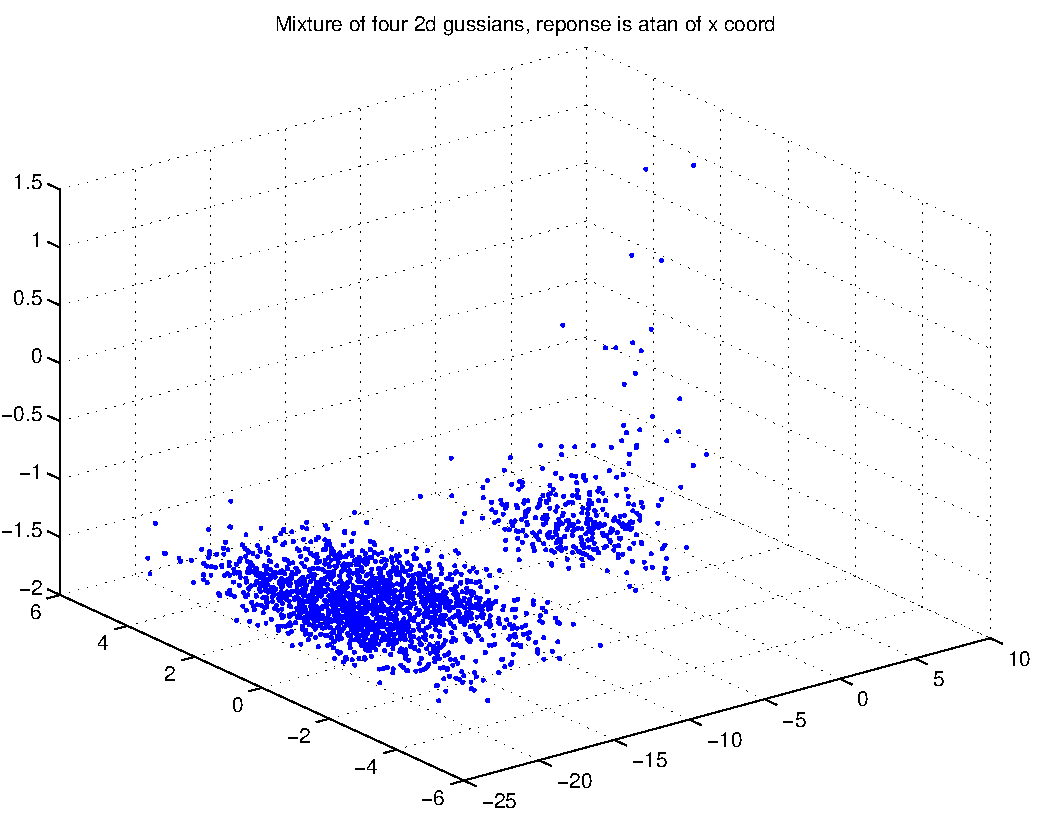
\includegraphics[width=10.0cm,height=10.0cm]{AtanDataSet.pdf}

\subsubsection{3 x 1 Linear Regression}
Sample size = 64

Number of features = 3

$\sigma = \left(
\begin{array}{
ccc}
+3.952 & -0.499 & -0.010 \\
-0.499 & +1.895 & +0.465 \\
-0.010 & +0.465 & +4.477 \\
\end{array}
\right)$ \newline 

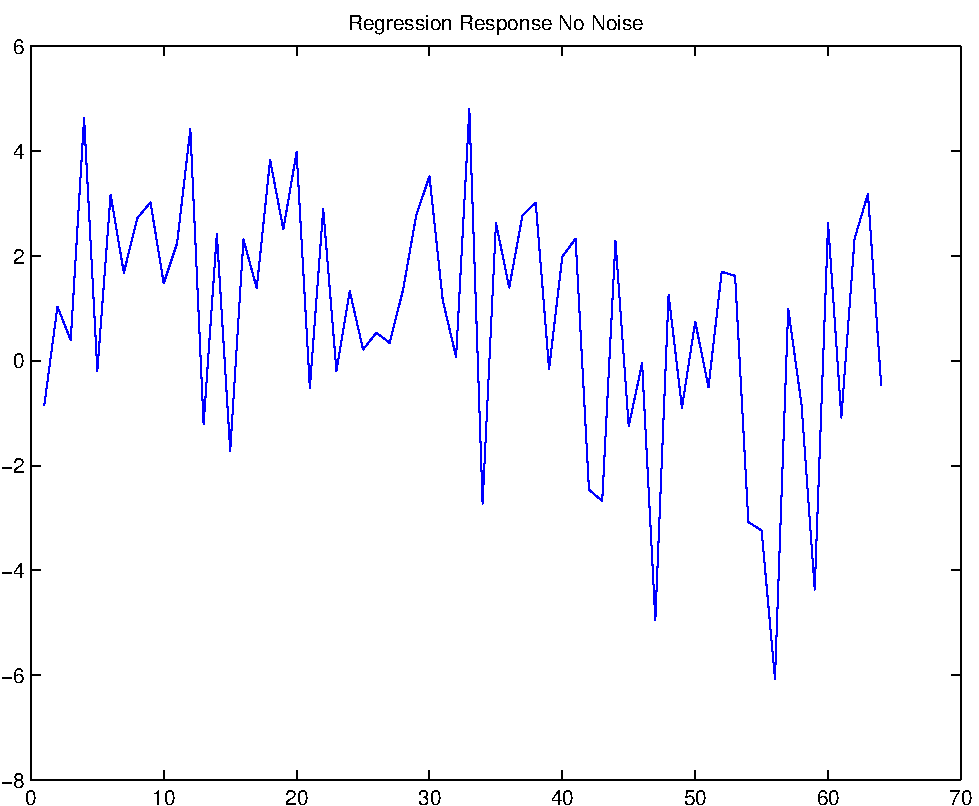
\includegraphics[width=10.0cm,height=10.0cm]{regression_response_no_noise.pdf}

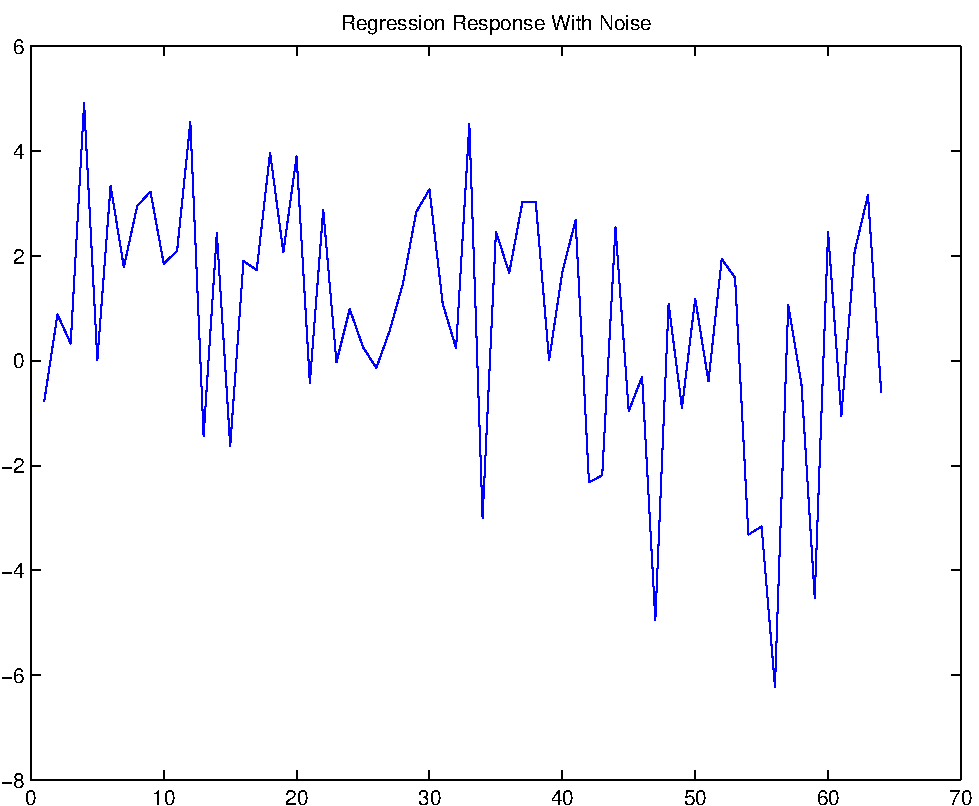
\includegraphics[width=10.0cm,height=10.0cm]{regression_response_with_noise.pdf}

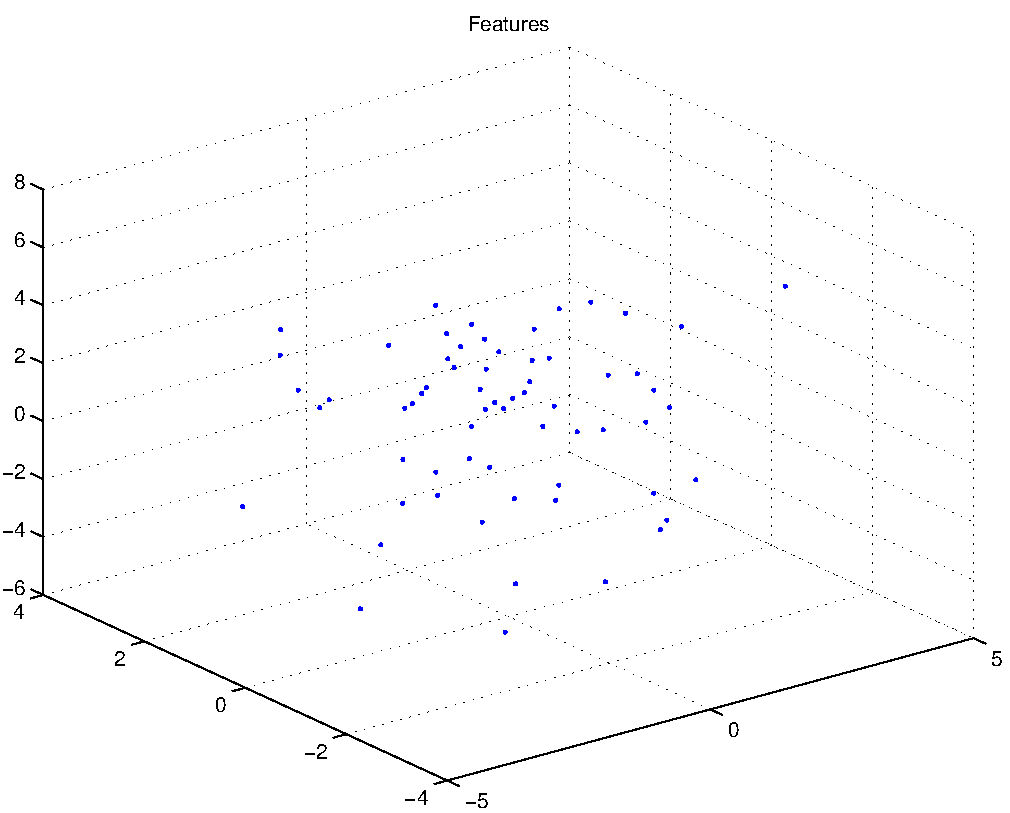
\includegraphics[width=10.0cm,height=10.0cm]{regression_features.pdf}

Beta
+0.817, +0.999, +0.510

Response
-3.176
+2.602
-2.518
+2.605
-1.161
+3.660
+2.267
+1.980
+2.602
-1.139
-0.975
+2.253
+0.822
+1.773
-1.114
+1.947
-2.384
+1.987
+0.121
-2.257
+1.845
-0.286
+1.823
+4.150
+2.464
+0.663
-0.492
+1.259
-1.387
+3.263
+0.954
-1.983
-1.751
+2.611
+4.006
+3.593
+0.152
+2.654
-1.383
-1.166
+0.287
+0.764
+0.566
-0.425
+0.982
+0.095
+0.938
-0.010
-0.692
-0.284
+0.280
+2.769
+1.769
+1.228
-3.392
+0.894
-2.089
-0.201
+1.019
-0.100
+3.920
-2.175
+1.056
-1.569
Estimate for Beta
+0.810
+0.998
+0.483
Error:
-0.008, -0.001, -0.027


QueryPerformanceCounter  =  +4.652
\subsubsection{Fast Gauss Transform}
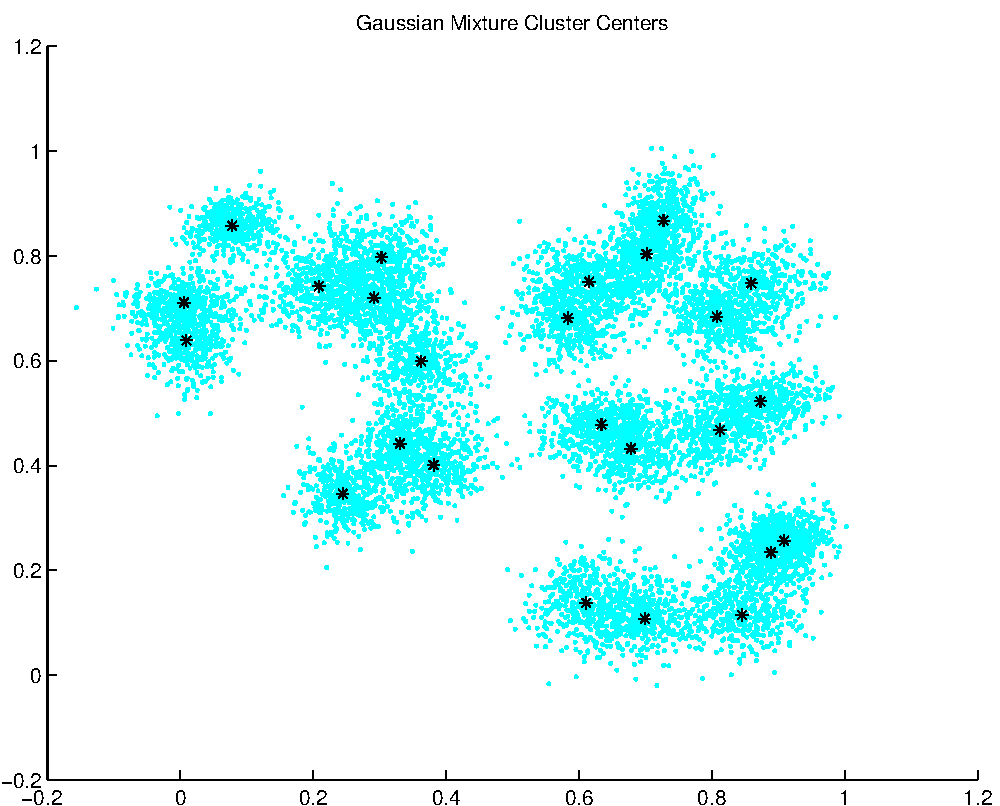
\includegraphics[width=10.0cm,height=10.0cm]{GaussianMixture_ClusterCenters25_Centers.pdf}

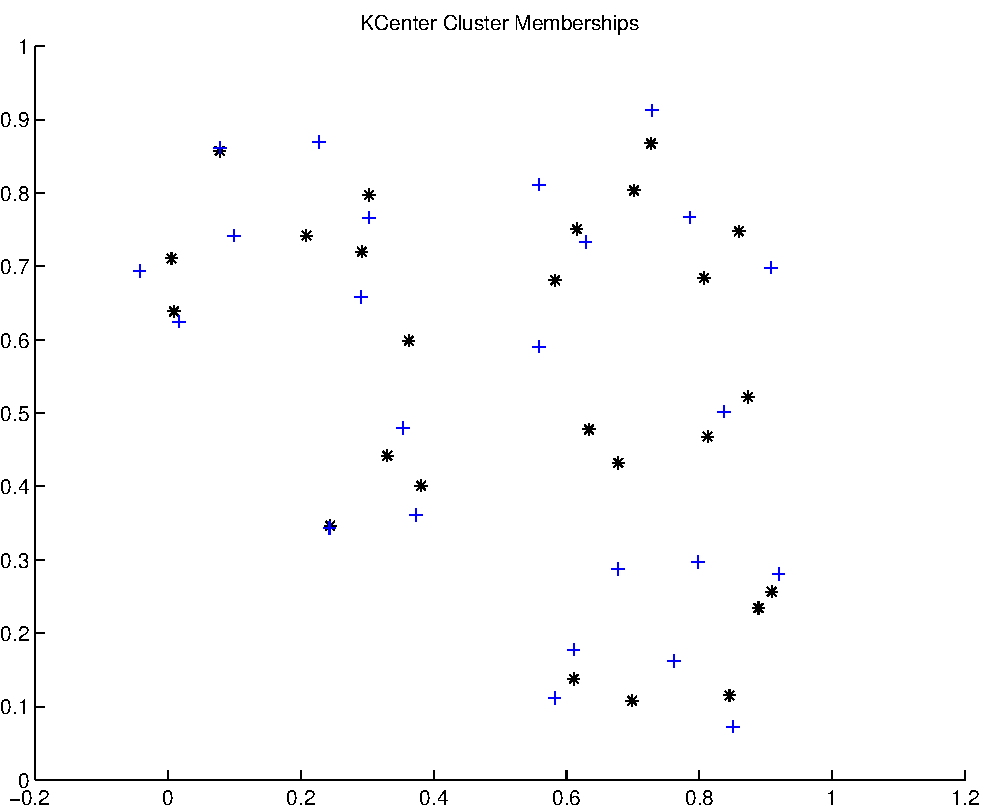
\includegraphics[width=10.0cm,height=10.0cm]{KCenterClusterMemberships_25_Centers.pdf}

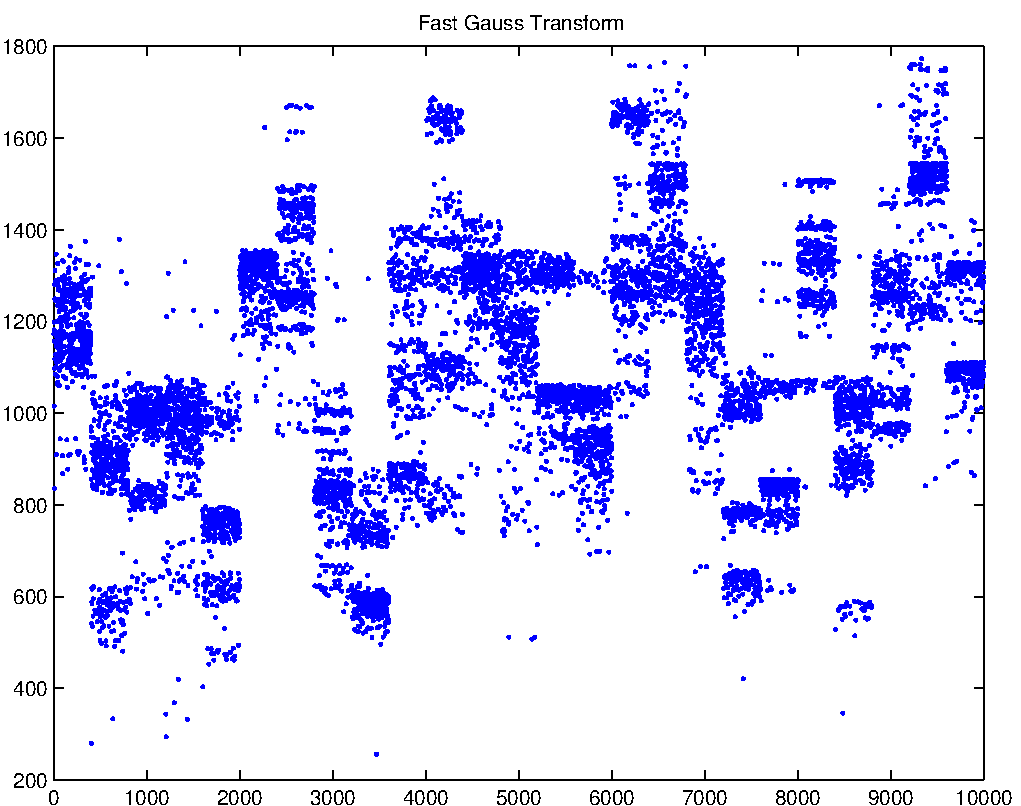
\includegraphics[width=10.0cm,height=10.0cm]{FGT25_Centers.pdf}

QueryPerformanceCounter  =  +7.074
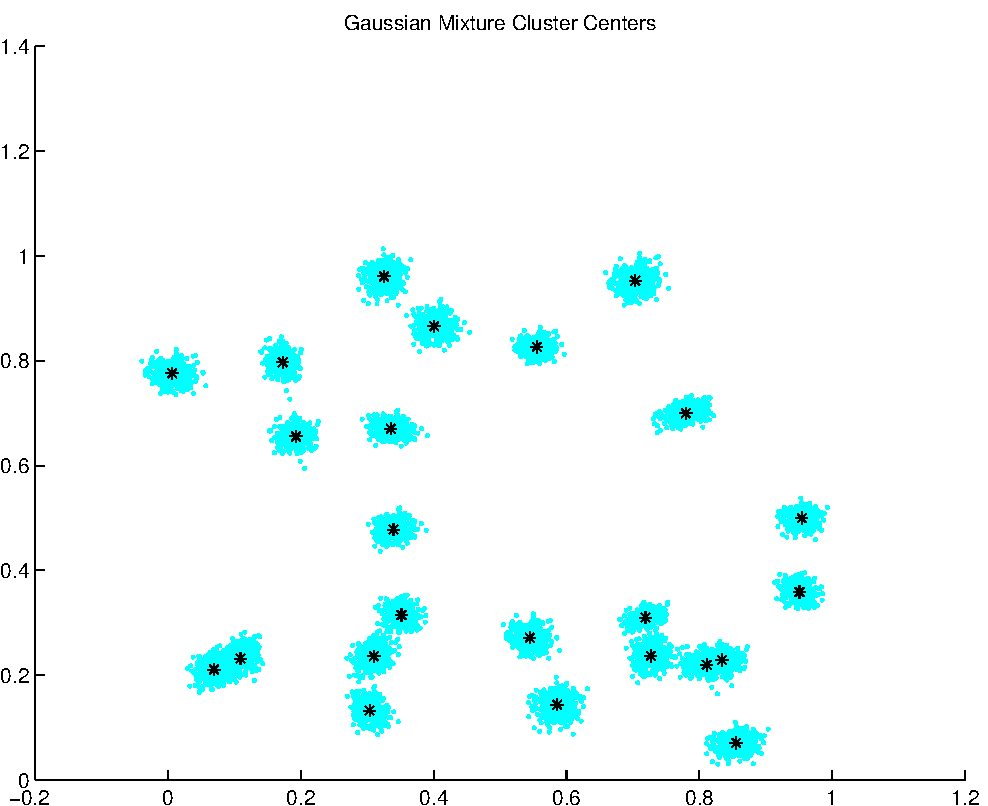
\includegraphics[width=10.0cm,height=10.0cm]{GaussianMixture_ClusterCenters24_Centers.pdf}

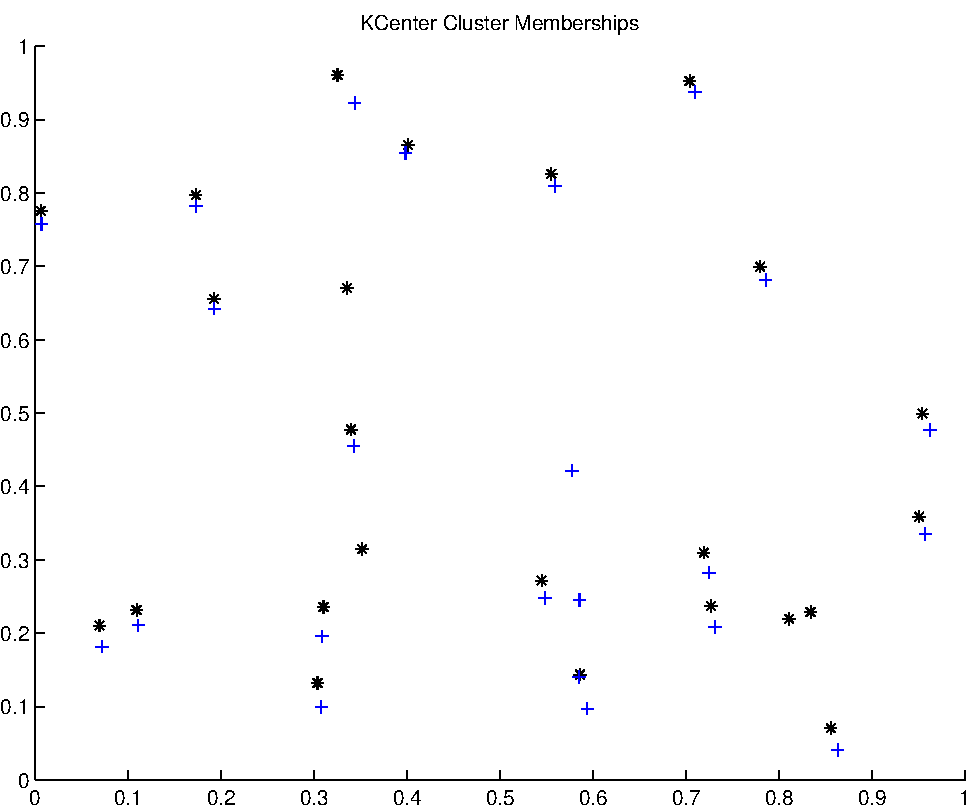
\includegraphics[width=10.0cm,height=10.0cm]{KCenterClusterMemberships_24_Centers.pdf}

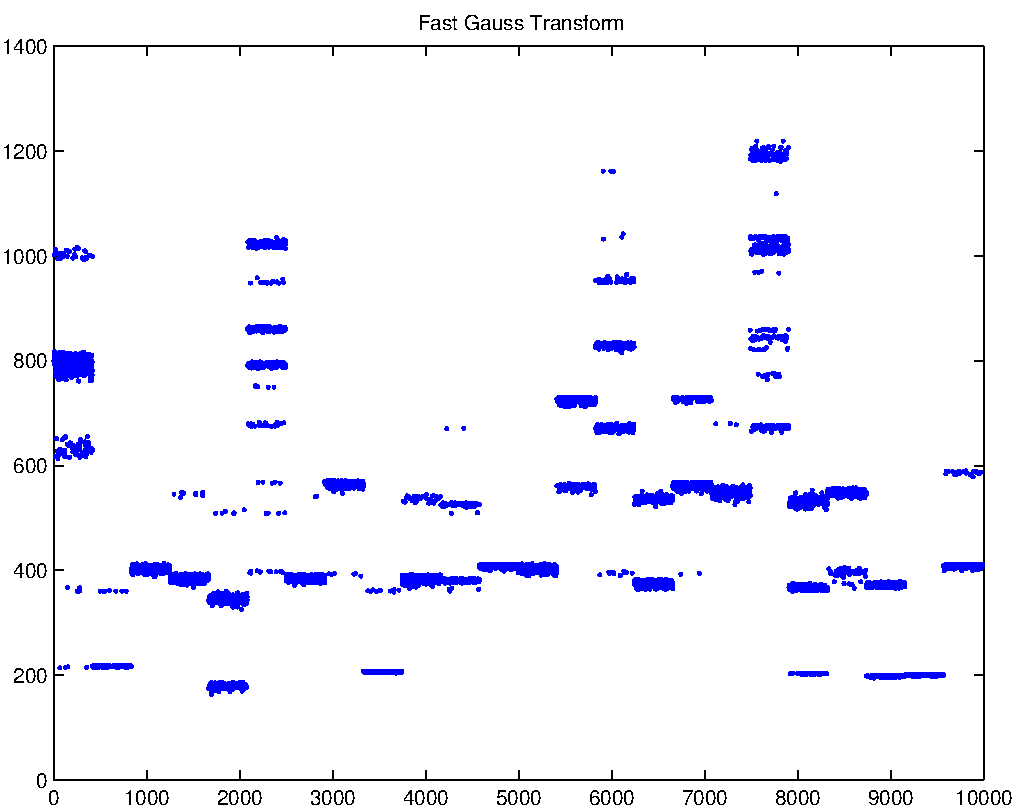
\includegraphics[width=10.0cm,height=10.0cm]{FGT24_Centers.pdf}

QueryPerformanceCounter  =  +7.295
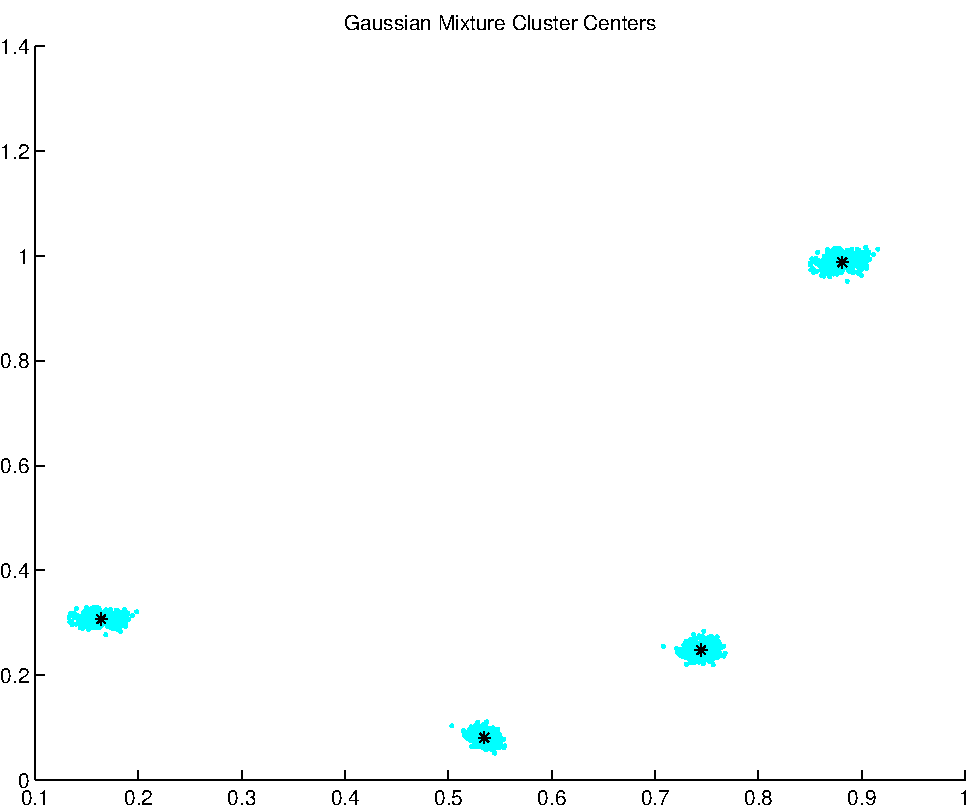
\includegraphics[width=10.0cm,height=10.0cm]{GaussianMixture_ClusterCenters4_Centers.pdf}

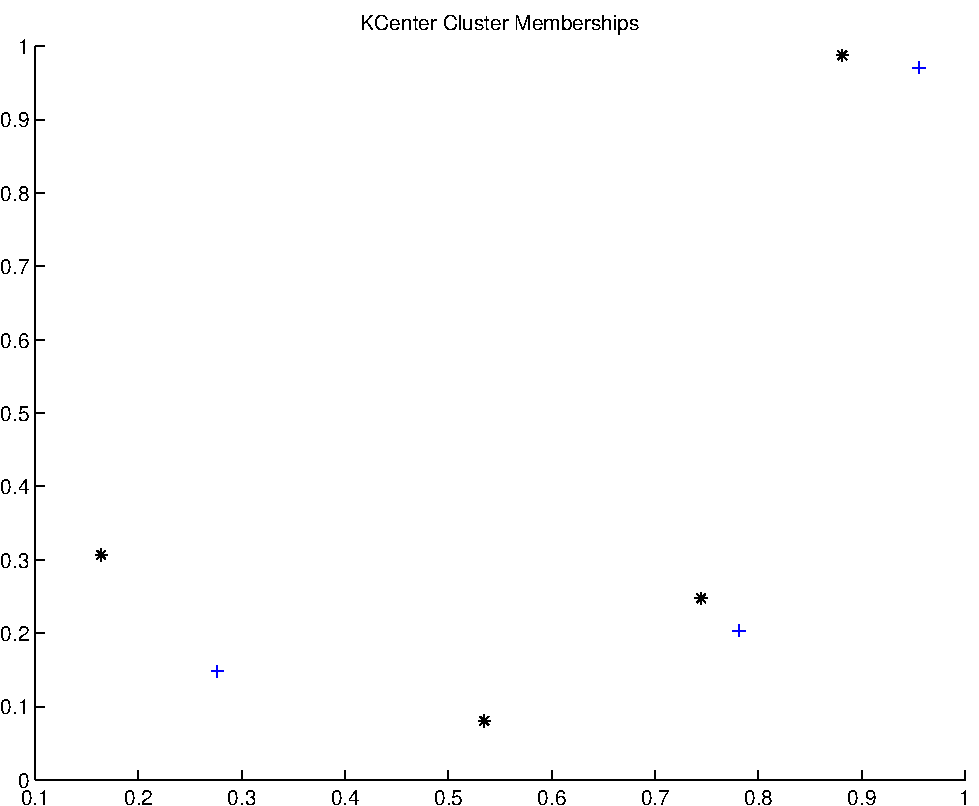
\includegraphics[width=10.0cm,height=10.0cm]{KCenterClusterMemberships_4_Centers.pdf}

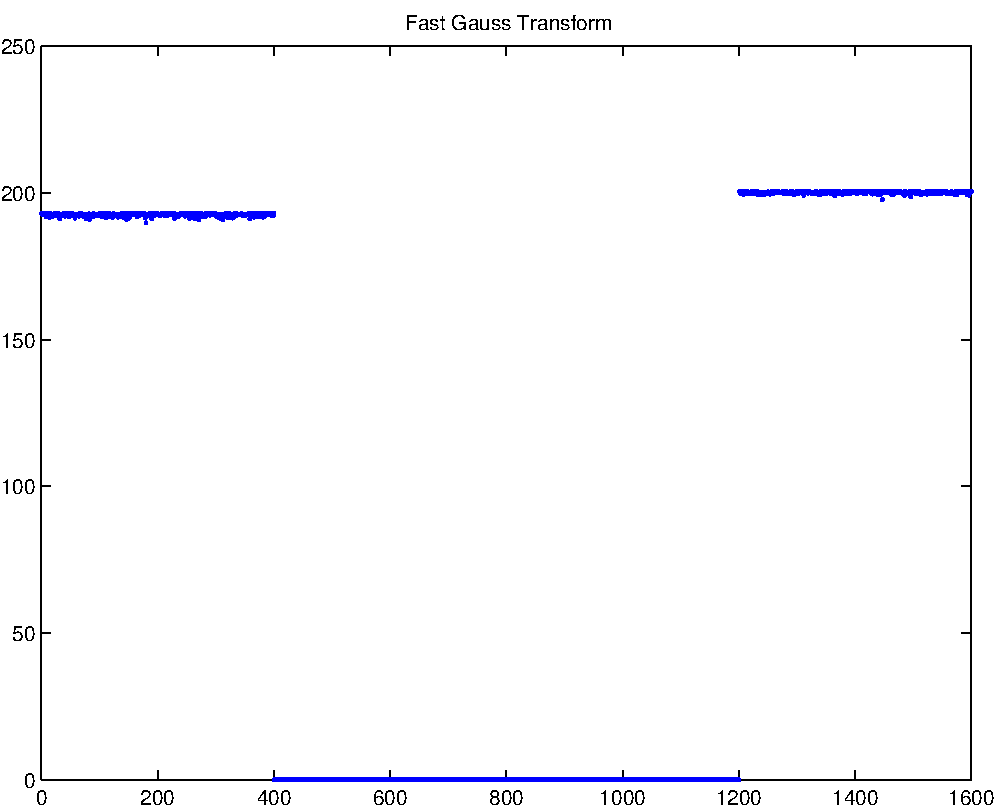
\includegraphics[width=10.0cm,height=10.0cm]{FGT4_Centers.pdf}

QueryPerformanceCounter  =  +3.909
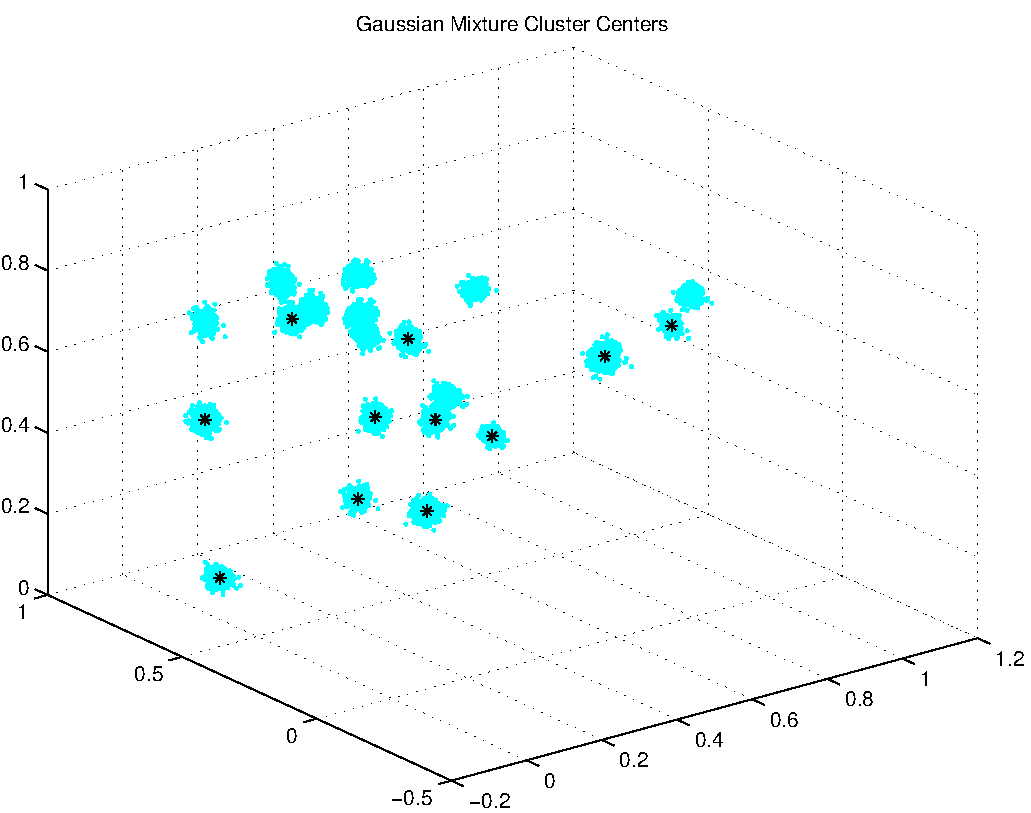
\includegraphics[width=10.0cm,height=10.0cm]{GaussianMixture_ClusterCenters20_Centers.pdf}

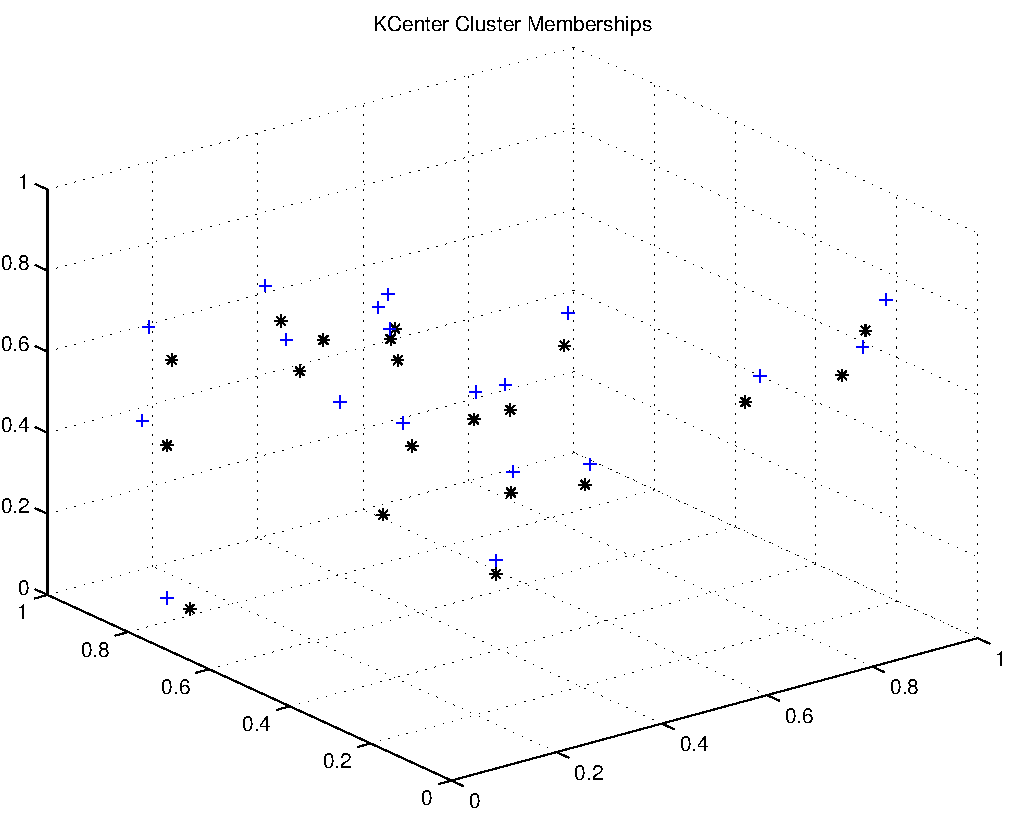
\includegraphics[width=10.0cm,height=10.0cm]{KCenterClusterMemberships_20_Centers.pdf}

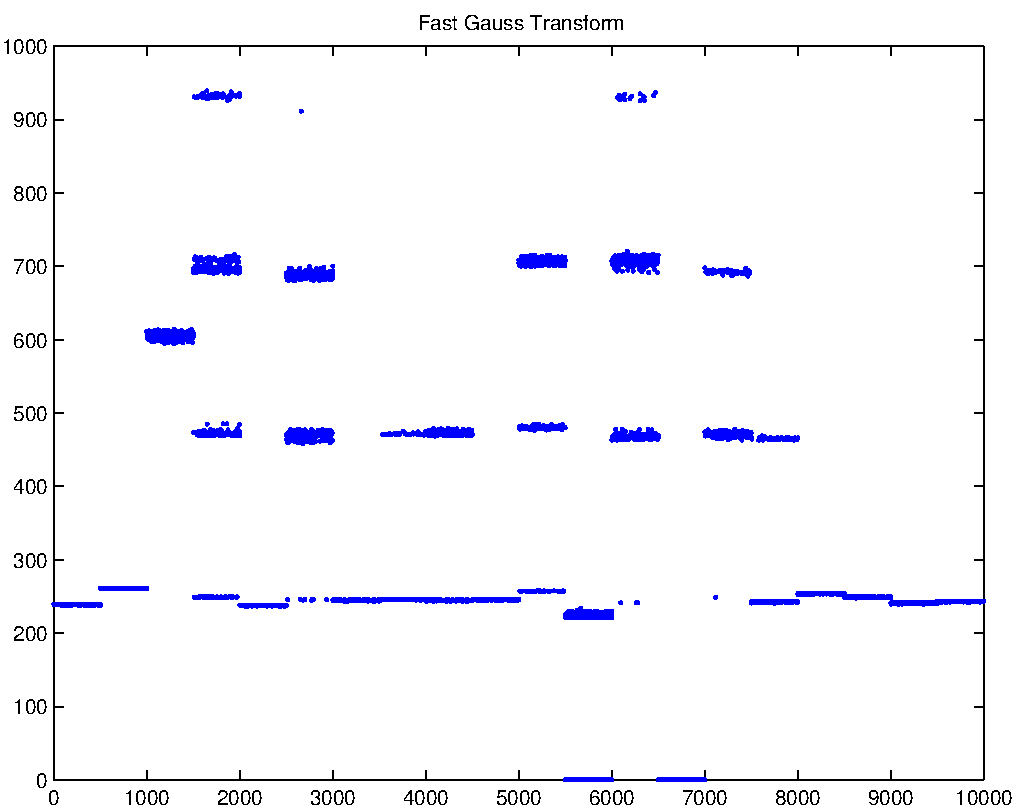
\includegraphics[width=10.0cm,height=10.0cm]{FGT20_Centers.pdf}

QueryPerformanceCounter  =  +6.636
\subsubsection{Matrix Norms}
\subsubsection{Haar Distributed Random Orthogonal Matrix $A \in O(n)$}
 Testing Operator Norm
Number of Dimensions: +12

$A = \left(
\begin{array}{
cccccccccccc}
-0.048 & +0.280 & +0.280 & +0.711 & -0.237 & -0.069 & -0.364 & -0.007 & -0.349 & -0.070 & +0.123 & -0.033 \\
+0.500 & -0.183 & +0.164 & -0.157 & -0.370 & +0.472 & -0.411 & +0.220 & +0.135 & -0.103 & -0.126 & +0.208 \\
-0.211 & -0.353 & +0.163 & +0.156 & -0.120 & -0.479 & +0.069 & +0.248 & +0.175 & -0.148 & -0.268 & +0.587 \\
+0.257 & +0.224 & -0.331 & +0.468 & +0.402 & +0.239 & +0.209 & +0.303 & +0.156 & -0.088 & -0.407 & +0.066 \\
-0.081 & +0.542 & -0.220 & -0.195 & -0.080 & -0.129 & -0.288 & +0.100 & +0.075 & +0.588 & -0.064 & +0.377 \\
+0.219 & +0.006 & -0.371 & +0.090 & -0.634 & -0.252 & +0.347 & +0.335 & +0.038 & +0.077 & +0.155 & -0.277 \\
-0.202 & +0.396 & +0.246 & -0.154 & -0.315 & +0.348 & +0.540 & -0.079 & -0.237 & -0.201 & -0.179 & +0.266 \\
+0.275 & +0.291 & -0.333 & -0.083 & -0.003 & -0.242 & -0.110 & -0.361 & +0.114 & -0.599 & +0.257 & +0.288 \\
+0.161 & -0.258 & -0.092 & +0.353 & -0.171 & +0.167 & +0.216 & -0.647 & +0.193 & +0.397 & +0.026 & +0.238 \\
+0.160 & +0.241 & +0.512 & +0.075 & +0.148 & -0.026 & +0.222 & +0.180 & +0.554 & +0.078 & +0.481 & +0.020 \\
+0.035 & +0.231 & +0.227 & -0.048 & -0.188 & -0.252 & -0.106 & -0.294 & +0.403 & -0.072 & -0.595 & -0.416 \\
+0.643 & +0.016 & +0.281 & -0.133 & +0.195 & -0.365 & +0.190 & -0.050 & -0.471 & +0.187 & -0.140 & +0.062 \\
\end{array}
\right)$ \newline 

$Det(A) :   A \in O(n)$ = (+1.000,+0.000)

$L = \left(
\begin{array}{
cccccccccccc}
+1.000 & +0.000 & +0.000 & +0.000 & +0.000 & +0.000 & +0.000 & +0.000 & +0.000 & +0.000 & +0.000 & +0.000 \\
-0.126 & +1.000 & +0.000 & +0.000 & +0.000 & +0.000 & +0.000 & +0.000 & +0.000 & +0.000 & +0.000 & +0.000 \\
+0.249 & +0.435 & +1.000 & +0.000 & +0.000 & +0.000 & +0.000 & +0.000 & +0.000 & +0.000 & +0.000 & +0.000 \\
+0.399 & +0.399 & -0.709 & +1.000 & +0.000 & +0.000 & +0.000 & +0.000 & +0.000 & +0.000 & +0.000 & +0.000 \\
+0.341 & +0.002 & -0.895 & +0.421 & +1.000 & +0.000 & +0.000 & +0.000 & +0.000 & +0.000 & +0.000 & +0.000 \\
+0.778 & -0.358 & -0.231 & -0.112 & +0.601 & +1.000 & +0.000 & +0.000 & +0.000 & +0.000 & +0.000 & +0.000 \\
-0.074 & +0.516 & +0.758 & +0.882 & +0.868 & -0.429 & +1.000 & +0.000 & +0.000 & +0.000 & +0.000 & +0.000 \\
-0.314 & +0.737 & +0.902 & -0.294 & +0.255 & +0.493 & -0.648 & +1.000 & +0.000 & +0.000 & +0.000 & +0.000 \\
+0.250 & -0.482 & -0.481 & +0.509 & +0.528 & +0.089 & +0.114 & +0.994 & +1.000 & +0.000 & +0.000 & +0.000 \\
+0.428 & +0.521 & -0.685 & +0.295 & +0.130 & -0.034 & +0.040 & +0.495 & +0.696 & +1.000 & +0.000 & +0.000 \\
+0.054 & +0.423 & +0.556 & -0.083 & +0.269 & -0.137 & +0.225 & +0.342 & +0.517 & +0.495 & +1.000 & +0.000 \\
-0.328 & -0.639 & +0.264 & -0.101 & +0.104 & -0.718 & +0.443 & -0.857 & -0.381 & -0.139 & +0.709 & +1.000 \\
\end{array}
\right)$ \newline 

$U = \left(
\begin{array}{
cccccccccccc}
+0.643 & +0.016 & +0.281 & -0.133 & +0.195 & -0.365 & +0.190 & -0.050 & -0.471 & +0.187 & -0.140 & +0.062 \\
+0.000 & +0.544 & -0.184 & -0.212 & -0.055 & -0.175 & -0.264 & +0.093 & +0.016 & +0.612 & -0.082 & +0.384 \\
+0.000 & +0.000 & +0.522 & +0.200 & +0.123 & +0.141 & +0.290 & +0.152 & +0.665 & -0.235 & +0.551 & -0.163 \\
+0.000 & +0.000 & +0.000 & +0.747 & +0.433 & +0.555 & +0.444 & +0.393 & +0.808 & -0.573 & +0.072 & -0.228 \\
+0.000 & +0.000 & +0.000 & +0.000 & -0.772 & -0.234 & +0.356 & +0.323 & +0.453 & +0.043 & +0.665 & -0.348 \\
+0.000 & +0.000 & +0.000 & +0.000 & +0.000 & +0.930 & -0.750 & +0.177 & +0.479 & -0.174 & -0.312 & +0.443 \\
+0.000 & +0.000 & +0.000 & +0.000 & +0.000 & +0.000 & -1.455 & -0.725 & -1.796 & +0.199 & -1.037 & +0.590 \\
+0.000 & +0.000 & +0.000 & +0.000 & +0.000 & +0.000 & +0.000 & -0.824 & -2.272 & -0.347 & -1.326 & +0.334 \\
+0.000 & +0.000 & +0.000 & +0.000 & +0.000 & +0.000 & +0.000 & +0.000 & +2.410 & +1.139 & +1.364 & +0.190 \\
+0.000 & +0.000 & +0.000 & +0.000 & +0.000 & +0.000 & +0.000 & +0.000 & +0.000 & -1.630 & +0.367 & -0.244 \\
+0.000 & +0.000 & +0.000 & +0.000 & +0.000 & +0.000 & +0.000 & +0.000 & +0.000 & +0.000 & -1.274 & -0.581 \\
+0.000 & +0.000 & +0.000 & +0.000 & +0.000 & +0.000 & +0.000 & +0.000 & +0.000 & +0.000 & +0.000 & +1.703 \\
\end{array}
\right)$ \newline 

$L * U  = \left(
\begin{array}{
cccccccccccc}
+0.643 & +0.016 & +0.281 & -0.133 & +0.195 & -0.365 & +0.190 & -0.050 & -0.471 & +0.187 & -0.140 & +0.062 \\
-0.081 & +0.542 & -0.220 & -0.195 & -0.080 & -0.129 & -0.288 & +0.100 & +0.075 & +0.588 & -0.064 & +0.377 \\
+0.160 & +0.241 & +0.512 & +0.075 & +0.148 & -0.026 & +0.222 & +0.180 & +0.554 & +0.078 & +0.481 & +0.020 \\
+0.257 & +0.224 & -0.331 & +0.468 & +0.402 & +0.239 & +0.209 & +0.303 & +0.156 & -0.088 & -0.407 & +0.066 \\
+0.219 & +0.006 & -0.371 & +0.090 & -0.634 & -0.252 & +0.347 & +0.335 & +0.038 & +0.077 & +0.155 & -0.277 \\
+0.500 & -0.183 & +0.164 & -0.157 & -0.370 & +0.472 & -0.411 & +0.220 & +0.135 & -0.103 & -0.126 & +0.208 \\
-0.048 & +0.280 & +0.280 & +0.711 & -0.237 & -0.069 & -0.364 & -0.007 & -0.349 & -0.070 & +0.123 & -0.033 \\
-0.202 & +0.396 & +0.246 & -0.154 & -0.315 & +0.348 & +0.540 & -0.079 & -0.237 & -0.201 & -0.179 & +0.266 \\
+0.161 & -0.258 & -0.092 & +0.353 & -0.171 & +0.167 & +0.216 & -0.647 & +0.193 & +0.397 & +0.026 & +0.238 \\
+0.275 & +0.291 & -0.333 & -0.083 & -0.003 & -0.242 & -0.110 & -0.361 & +0.114 & -0.599 & +0.257 & +0.288 \\
+0.035 & +0.231 & +0.227 & -0.048 & -0.188 & -0.252 & -0.106 & -0.294 & +0.403 & -0.072 & -0.595 & -0.416 \\
-0.211 & -0.353 & +0.163 & +0.156 & -0.120 & -0.479 & +0.069 & +0.248 & +0.175 & -0.148 & -0.268 & +0.587 \\
\end{array}
\right)$ \newline 

$Det(L) :    = (+1.000,+0.000)     Det(U) :    = (-1.000,+0.000)     Det(LU) :    = (-1.000,+0.000)$

$||A||_{L_1}$  = +3.220

$||A||_{L_{\infty}}$ = +3.164

$||A^{-1}||_{L_1}$  = +3.164

$||A^{-1}||_{L_{\infty}}$ = +3.220

$||A||_{L_{\infty}} * ||A^{-1}||_{L_{\infty}} = +10.189$

$||A||_{L_1} * ||A^{-1}||_{L_1} = +10.189$

Frobenious Norm  $||A||_{\textit{F}}$ via $\sum\limits_{i,j =0}^{n} \|A_{i,j}|$   of  $A \in O(n)$  +3.464

$L_1$ condition number of Haar Distributed Random Orthogonal Matrix $A \in O(n)$ +9.401

$A = \left(
\begin{array}{
cccccccccccc}
-0.048 & +0.280 & +0.280 & +0.711 & -0.237 & -0.069 & -0.364 & -0.007 & -0.349 & -0.070 & +0.123 & -0.033 \\
+0.500 & -0.183 & +0.164 & -0.157 & -0.370 & +0.472 & -0.411 & +0.220 & +0.135 & -0.103 & -0.126 & +0.208 \\
-0.211 & -0.353 & +0.163 & +0.156 & -0.120 & -0.479 & +0.069 & +0.248 & +0.175 & -0.148 & -0.268 & +0.587 \\
+0.257 & +0.224 & -0.331 & +0.468 & +0.402 & +0.239 & +0.209 & +0.303 & +0.156 & -0.088 & -0.407 & +0.066 \\
-0.081 & +0.542 & -0.220 & -0.195 & -0.080 & -0.129 & -0.288 & +0.100 & +0.075 & +0.588 & -0.064 & +0.377 \\
+0.219 & +0.006 & -0.371 & +0.090 & -0.634 & -0.252 & +0.347 & +0.335 & +0.038 & +0.077 & +0.155 & -0.277 \\
-0.202 & +0.396 & +0.246 & -0.154 & -0.315 & +0.348 & +0.540 & -0.079 & -0.237 & -0.201 & -0.179 & +0.266 \\
+0.275 & +0.291 & -0.333 & -0.083 & -0.003 & -0.242 & -0.110 & -0.361 & +0.114 & -0.599 & +0.257 & +0.288 \\
+0.161 & -0.258 & -0.092 & +0.353 & -0.171 & +0.167 & +0.216 & -0.647 & +0.193 & +0.397 & +0.026 & +0.238 \\
+0.160 & +0.241 & +0.512 & +0.075 & +0.148 & -0.026 & +0.222 & +0.180 & +0.554 & +0.078 & +0.481 & +0.020 \\
+0.035 & +0.231 & +0.227 & -0.048 & -0.188 & -0.252 & -0.106 & -0.294 & +0.403 & -0.072 & -0.595 & -0.416 \\
+0.643 & +0.016 & +0.281 & -0.133 & +0.195 & -0.365 & +0.190 & -0.050 & -0.471 & +0.187 & -0.140 & +0.062 \\
\end{array}
\right)$ \newline 

$L_{\infty}$ condition number of Haar Distributed Random Orthogonal Matrix $A \in O(n)$ +9.621

Eigenvalues of $A \in O(n)$

(+0.210,+0.978), (+0.210,-0.978), (-0.421,+0.907), (-0.421,-0.907), (-0.644,+0.765), (-0.644,-0.765), (-1.000,+0.024), (-1.000,-0.024), (+0.995,+0.097), (+0.995,-0.097), (+0.852,+0.523), (+0.852,-0.523)

 $|\lambda | : \lambda \in \sigma(A) , A \in O(n)$

+1.000, +1.000, +1.000, +1.000, +1.000, +1.000, +1.000, +1.000, +1.000, +1.000, +1.000, +1.000


Calculating $A^{\dag} A,$  we expect $A^{\dag} A \approx I$

$A^{\dag} A = \left(
\begin{array}{
cccccccccccc}
+1.000 & -0.000 & -0.000 & +0.000 & -0.000 & -0.000 & -0.000 & +0.000 & +0.000 & -0.000 & -0.000 & +0.000 \\
-0.000 & +1.000 & -0.000 & +0.000 & +0.000 & -0.000 & +0.000 & +0.000 & -0.000 & -0.000 & -0.000 & +0.000 \\
-0.000 & -0.000 & +1.000 & +0.000 & -0.000 & -0.000 & -0.000 & -0.000 & -0.000 & -0.000 & -0.000 & +0.000 \\
+0.000 & +0.000 & +0.000 & +1.000 & +0.000 & +0.000 & +0.000 & -0.000 & +0.000 & +0.000 & +0.000 & -0.000 \\
-0.000 & +0.000 & -0.000 & +0.000 & +1.000 & -0.000 & -0.000 & +0.000 & -0.000 & -0.000 & -0.000 & +0.000 \\
-0.000 & -0.000 & -0.000 & +0.000 & -0.000 & +1.000 & +0.000 & -0.000 & +0.000 & +0.000 & -0.000 & +0.000 \\
-0.000 & +0.000 & -0.000 & +0.000 & -0.000 & +0.000 & +1.000 & +0.000 & -0.000 & -0.000 & -0.000 & +0.000 \\
+0.000 & +0.000 & -0.000 & -0.000 & +0.000 & -0.000 & +0.000 & +1.000 & -0.000 & -0.000 & +0.000 & -0.000 \\
+0.000 & -0.000 & -0.000 & +0.000 & -0.000 & +0.000 & -0.000 & -0.000 & +1.000 & +0.000 & -0.000 & -0.000 \\
-0.000 & -0.000 & -0.000 & +0.000 & -0.000 & +0.000 & -0.000 & -0.000 & +0.000 & +1.000 & -0.000 & -0.000 \\
-0.000 & -0.000 & -0.000 & +0.000 & -0.000 & -0.000 & -0.000 & +0.000 & -0.000 & -0.000 & +1.000 & +0.000 \\
+0.000 & +0.000 & +0.000 & -0.000 & +0.000 & +0.000 & +0.000 & -0.000 & -0.000 & -0.000 & +0.000 & +1.000 \\
\end{array}
\right)$ \newline 

Calculating $A^{-1} ,  A \in O(n)$.

$A^{-1} = \left(
\begin{array}{
cccccccccccc}
-0.048 & +0.500 & -0.211 & +0.257 & -0.081 & +0.219 & -0.202 & +0.275 & +0.161 & +0.160 & +0.035 & +0.643 \\
+0.280 & -0.183 & -0.353 & +0.224 & +0.542 & +0.006 & +0.396 & +0.291 & -0.258 & +0.241 & +0.231 & +0.016 \\
+0.280 & +0.164 & +0.163 & -0.331 & -0.220 & -0.371 & +0.246 & -0.333 & -0.092 & +0.512 & +0.227 & +0.281 \\
+0.711 & -0.157 & +0.156 & +0.468 & -0.195 & +0.090 & -0.154 & -0.083 & +0.353 & +0.075 & -0.048 & -0.133 \\
-0.237 & -0.370 & -0.120 & +0.402 & -0.080 & -0.634 & -0.315 & -0.003 & -0.171 & +0.148 & -0.188 & +0.195 \\
-0.069 & +0.472 & -0.479 & +0.239 & -0.129 & -0.252 & +0.348 & -0.242 & +0.167 & -0.026 & -0.252 & -0.365 \\
-0.364 & -0.411 & +0.069 & +0.209 & -0.288 & +0.347 & +0.540 & -0.110 & +0.216 & +0.222 & -0.106 & +0.190 \\
-0.007 & +0.220 & +0.248 & +0.303 & +0.100 & +0.335 & -0.079 & -0.361 & -0.647 & +0.180 & -0.294 & -0.050 \\
-0.349 & +0.135 & +0.175 & +0.156 & +0.075 & +0.038 & -0.237 & +0.114 & +0.193 & +0.554 & +0.403 & -0.471 \\
-0.070 & -0.103 & -0.148 & -0.088 & +0.588 & +0.077 & -0.201 & -0.599 & +0.397 & +0.078 & -0.072 & +0.187 \\
+0.123 & -0.126 & -0.268 & -0.407 & -0.064 & +0.155 & -0.179 & +0.257 & +0.026 & +0.481 & -0.595 & -0.140 \\
-0.033 & +0.208 & +0.587 & +0.066 & +0.377 & -0.277 & +0.266 & +0.288 & +0.238 & +0.020 & -0.416 & +0.062 \\
\end{array}
\right)$ \newline 

Calculating $A^{-1} *A  ,  A \in O(n)$.   We expect $A^{-1} *A  \approx I$. 

$A^{-1} *A = \left(
\begin{array}{
cccccccccccc}
+1.000 & +0.000 & -0.000 & +0.000 & +0.000 & -0.000 & +0.000 & -0.000 & +0.000 & +0.000 & -0.000 & -0.000 \\
+0.000 & +1.000 & +0.000 & +0.000 & +0.000 & +0.000 & -0.000 & +0.000 & +0.000 & +0.000 & +0.000 & -0.000 \\
-0.000 & -0.000 & +1.000 & -0.000 & +0.000 & -0.000 & -0.000 & -0.000 & -0.000 & +0.000 & -0.000 & +0.000 \\
+0.000 & -0.000 & +0.000 & +1.000 & -0.000 & -0.000 & -0.000 & -0.000 & -0.000 & +0.000 & -0.000 & +0.000 \\
+0.000 & -0.000 & -0.000 & +0.000 & +1.000 & -0.000 & +0.000 & +0.000 & -0.000 & +0.000 & +0.000 & -0.000 \\
+0.000 & +0.000 & +0.000 & +0.000 & +0.000 & +1.000 & +0.000 & -0.000 & -0.000 & -0.000 & -0.000 & -0.000 \\
-0.000 & +0.000 & +0.000 & +0.000 & +0.000 & +0.000 & +1.000 & -0.000 & -0.000 & +0.000 & -0.000 & +0.000 \\
-0.000 & +0.000 & -0.000 & -0.000 & -0.000 & -0.000 & -0.000 & +1.000 & -0.000 & -0.000 & +0.000 & -0.000 \\
+0.000 & +0.000 & -0.000 & +0.000 & +0.000 & -0.000 & +0.000 & +0.000 & +1.000 & +0.000 & -0.000 & +0.000 \\
+0.000 & +0.000 & +0.000 & +0.000 & +0.000 & +0.000 & +0.000 & -0.000 & -0.000 & +1.000 & -0.000 & -0.000 \\
-0.000 & +0.000 & -0.000 & -0.000 & -0.000 & +0.000 & +0.000 & +0.000 & +0.000 & -0.000 & +1.000 & -0.000 \\
+0.000 & +0.000 & -0.000 & +0.000 & -0.000 & -0.000 & -0.000 & -0.000 & +0.000 & +0.000 & +0.000 & +1.000 \\
\end{array}
\right)$ \newline 

Calculating SVD of  $A \in O(n)$

$U = \left(
\begin{array}{
cccccccccccc}
-0.267 & +0.154 & -0.069 & -0.280 & -0.522 & +0.013 & -0.086 & +0.021 & -0.098 & -0.401 & -0.299 & +0.530 \\
+0.005 & -0.294 & +0.585 & +0.182 & +0.030 & +0.436 & +0.407 & -0.230 & +0.002 & +0.051 & -0.087 & +0.344 \\
-0.022 & -0.258 & -0.137 & -0.161 & +0.108 & +0.157 & -0.056 & +0.152 & -0.424 & -0.156 & +0.741 & +0.269 \\
-0.856 & +0.113 & -0.014 & +0.057 & +0.075 & +0.144 & +0.255 & +0.297 & -0.045 & +0.162 & +0.024 & -0.208 \\
-0.015 & +0.578 & -0.119 & -0.078 & +0.214 & -0.165 & +0.392 & -0.559 & -0.278 & +0.043 & +0.117 & +0.116 \\
-0.034 & -0.315 & -0.644 & +0.429 & -0.359 & +0.131 & +0.235 & -0.295 & +0.088 & +0.059 & +0.032 & -0.010 \\
-0.048 & +0.280 & +0.280 & +0.711 & -0.237 & -0.069 & -0.364 & -0.007 & -0.349 & -0.070 & +0.123 & -0.033 \\
+0.017 & +0.367 & -0.213 & +0.062 & +0.275 & +0.712 & -0.348 & -0.064 & +0.298 & -0.091 & +0.014 & +0.100 \\
+0.030 & +0.112 & +0.209 & -0.372 & -0.582 & +0.282 & -0.080 & -0.250 & +0.008 & +0.264 & +0.278 & -0.412 \\
+0.287 & +0.026 & -0.145 & -0.051 & +0.009 & +0.357 & +0.205 & +0.251 & -0.622 & -0.118 & -0.399 & -0.316 \\
-0.267 & -0.332 & -0.054 & -0.139 & +0.212 & -0.001 & -0.497 & -0.422 & -0.350 & +0.341 & -0.293 & +0.054 \\
-0.193 & -0.202 & +0.115 & -0.023 & +0.137 & -0.016 & -0.028 & -0.359 & +0.060 & -0.753 & +0.029 & -0.433 \\
\end{array}
\right)$ \newline 

$S = \left(
\begin{array}{
cccccccccccc}
+1.000 & +0.000 & +0.000 & +0.000 & +0.000 & +0.000 & +0.000 & +0.000 & +0.000 & +0.000 & +0.000 & +0.000 \\
+0.000 & +1.000 & +0.000 & +0.000 & +0.000 & +0.000 & +0.000 & +0.000 & +0.000 & +0.000 & +0.000 & +0.000 \\
+0.000 & +0.000 & +1.000 & +0.000 & +0.000 & +0.000 & +0.000 & +0.000 & +0.000 & +0.000 & +0.000 & +0.000 \\
+0.000 & +0.000 & +0.000 & +1.000 & +0.000 & +0.000 & +0.000 & +0.000 & +0.000 & +0.000 & +0.000 & +0.000 \\
+0.000 & +0.000 & +0.000 & +0.000 & +1.000 & +0.000 & +0.000 & +0.000 & +0.000 & +0.000 & +0.000 & +0.000 \\
+0.000 & +0.000 & +0.000 & +0.000 & +0.000 & +1.000 & +0.000 & +0.000 & +0.000 & +0.000 & +0.000 & +0.000 \\
+0.000 & +0.000 & +0.000 & +0.000 & +0.000 & +0.000 & +1.000 & +0.000 & +0.000 & +0.000 & +0.000 & +0.000 \\
+0.000 & +0.000 & +0.000 & +0.000 & +0.000 & +0.000 & +0.000 & +1.000 & +0.000 & +0.000 & +0.000 & +0.000 \\
+0.000 & +0.000 & +0.000 & +0.000 & +0.000 & +0.000 & +0.000 & +0.000 & +1.000 & +0.000 & +0.000 & +0.000 \\
+0.000 & +0.000 & +0.000 & +0.000 & +0.000 & +0.000 & +0.000 & +0.000 & +0.000 & +1.000 & +0.000 & +0.000 \\
+0.000 & +0.000 & +0.000 & +0.000 & +0.000 & +0.000 & +0.000 & +0.000 & +0.000 & +0.000 & +1.000 & +0.000 \\
+0.000 & +0.000 & +0.000 & +0.000 & +0.000 & +0.000 & +0.000 & +0.000 & +0.000 & +0.000 & +0.000 & +1.000 \\
\end{array}
\right)$ \newline 

$V = \left(
\begin{array}{
cccccccccccc}
-0.000 & -0.000 & +0.000 & +0.000 & +0.000 & +0.000 & +1.000 & +0.000 & +0.000 & +0.000 & +0.000 & -0.000 \\
+0.286 & +0.178 & +0.051 & -0.529 & -0.594 & -0.099 & +0.000 & +0.329 & +0.267 & +0.173 & -0.061 & -0.171 \\
+0.436 & +0.202 & -0.098 & +0.000 & -0.310 & -0.005 & +0.000 & -0.452 & -0.557 & -0.368 & -0.022 & -0.113 \\
-0.185 & +0.013 & -0.314 & +0.000 & +0.000 & +0.177 & +0.000 & +0.430 & -0.631 & +0.367 & -0.298 & -0.172 \\
+0.217 & -0.357 & -0.144 & +0.066 & +0.232 & -0.160 & +0.000 & +0.218 & +0.076 & -0.257 & +0.178 & -0.755 \\
+0.020 & -0.371 & -0.034 & +0.000 & -0.129 & +0.461 & +0.000 & -0.426 & +0.261 & +0.165 & -0.548 & -0.233 \\
+0.561 & +0.475 & -0.057 & +0.264 & +0.412 & -0.076 & +0.000 & +0.031 & +0.191 & +0.296 & -0.291 & -0.028 \\
+0.322 & -0.315 & +0.204 & -0.529 & +0.414 & +0.107 & +0.000 & +0.187 & -0.170 & -0.254 & -0.237 & +0.329 \\
-0.176 & +0.491 & -0.144 & -0.264 & +0.207 & +0.650 & +0.000 & +0.033 & +0.132 & -0.279 & +0.201 & -0.188 \\
-0.373 & +0.256 & -0.006 & +0.000 & +0.000 & -0.368 & +0.000 & +0.086 & +0.105 & -0.495 & -0.623 & -0.092 \\
+0.068 & -0.129 & -0.895 & -0.132 & +0.000 & -0.129 & +0.000 & -0.064 & +0.203 & -0.075 & +0.032 & +0.302 \\
-0.230 & +0.116 & -0.006 & -0.529 & +0.311 & -0.359 & +0.000 & -0.474 & -0.109 & +0.356 & +0.067 & -0.248 \\
\end{array}
\right)$ \newline 

$U S V = \left(
\begin{array}{
cccccccccccc}
-0.064 & +0.094 & +0.467 & -0.365 & -0.076 & -0.034 & -0.267 & -0.427 & +0.027 & +0.492 & +0.251 & +0.264 \\
+0.203 & +0.227 & -0.144 & +0.215 & +0.124 & +0.070 & +0.005 & -0.646 & -0.336 & +0.147 & -0.358 & -0.375 \\
+0.062 & -0.559 & -0.539 & -0.080 & +0.237 & -0.337 & -0.022 & -0.311 & +0.170 & +0.126 & +0.034 & +0.272 \\
+0.271 & -0.042 & +0.005 & -0.026 & +0.091 & +0.048 & -0.856 & +0.196 & +0.082 & -0.093 & -0.357 & +0.025 \\
+0.225 & +0.297 & -0.162 & +0.105 & -0.327 & -0.524 & -0.015 & +0.167 & +0.392 & +0.379 & +0.067 & -0.335 \\
-0.522 & +0.156 & -0.156 & +0.339 & +0.276 & +0.214 & -0.034 & +0.201 & +0.131 & +0.538 & -0.248 & +0.180 \\
-0.085 & -0.154 & -0.239 & -0.163 & -0.534 & -0.076 & -0.048 & +0.227 & -0.659 & +0.260 & -0.157 & +0.119 \\
-0.182 & -0.352 & -0.092 & -0.367 & -0.258 & +0.469 & +0.017 & -0.068 & +0.351 & +0.122 & -0.138 & -0.502 \\
-0.041 & +0.189 & -0.120 & +0.192 & -0.566 & +0.145 & +0.030 & -0.313 & +0.334 & -0.258 & -0.259 & +0.475 \\
+0.357 & -0.463 & +0.508 & +0.292 & -0.054 & -0.032 & +0.287 & +0.100 & +0.069 & +0.242 & -0.382 & +0.093 \\
-0.560 & -0.291 & +0.254 & +0.383 & -0.172 & -0.368 & -0.267 & -0.181 & -0.054 & -0.213 & +0.058 & -0.265 \\
+0.267 & -0.174 & -0.133 & +0.507 & -0.165 & +0.418 & -0.193 & -0.019 & -0.060 & +0.160 & +0.596 & -0.017 \\
\end{array}
\right)$ \newline 

\subsubsection{Wishart Matrix $A \in W(n)$}
$L_1$ condition number of Wishart Matrix +56267.800
$L_infty$ condition number of Wishart Matrix +56267.800
\subsubsection{Gaussian Orthogonal Ensemble $A \in GOE(n)$}
$L_1$ condition number of GOE Matrix +470.231
$L_\infty$ condition number of GOE Matrix +470.231
\subsubsection{The Identity Matrix $I \in M(n)$}
$L_1$ condition number of $I$ = +1.000
$L_\infty$ condition number of $I$ = +1.000
QueryPerformanceCounter  =  +0.318
\subsubsection{Principal Components Matlab }
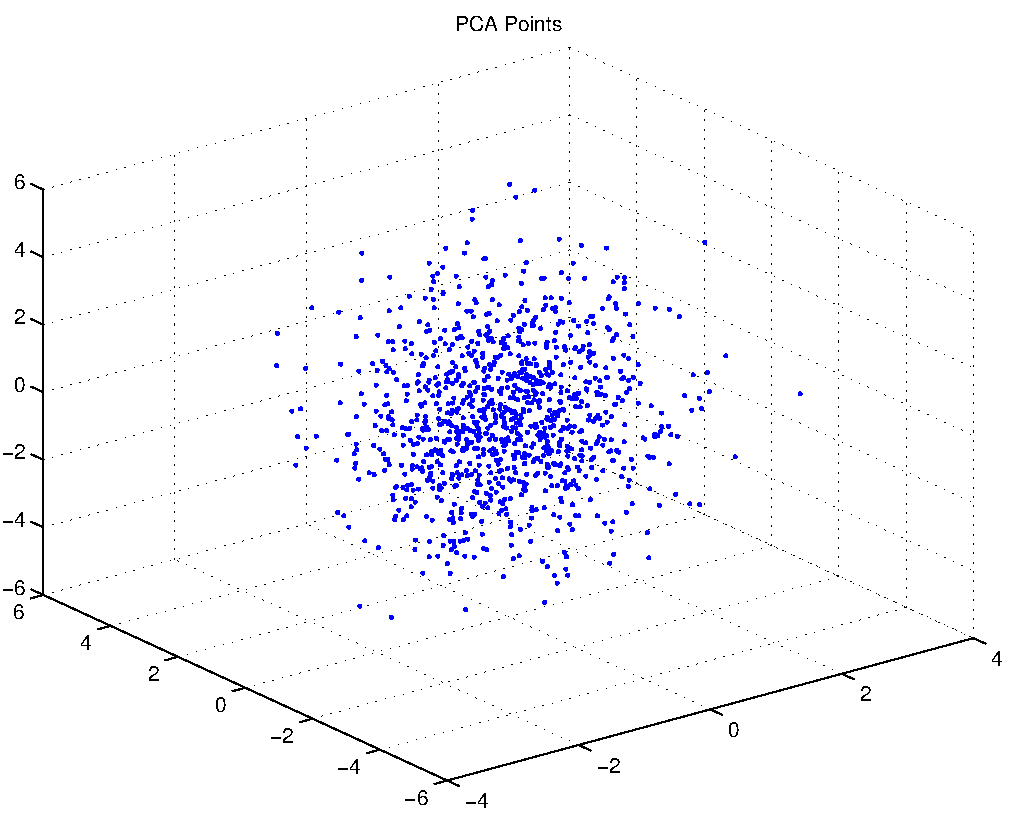
\includegraphics[width=10.0cm,height=10.0cm]{PCAPoints.pdf}

The eigenvectors:
+0.111, +0.093, +0.989
+0.212, +0.970, -0.115
-0.971, +0.223, +0.088

All of the eigenvalues of the covariance matrix:
(+0.958,+0.000), (+2.025,+0.000), (+3.017,+0.000)

QueryPerformanceCounter  =  +1.170
\subsubsection{Multi Variate Random Number Generator }
Sample from $N(\mu,\Sigma)$
mean= -0.002, variance=+1.004, skewness=+0.006, kurtosis=+3.003
mean= -0.001, variance=+1.017, skewness=-0.005, kurtosis=+2.988
mean= -0.002, variance=+1.006, skewness=-0.016, kurtosis=+3.014
Covariance Matrix 
+1.004, +0.009, +0.003
+0.009, +1.017, -0.003
+0.003, -0.003, +1.006

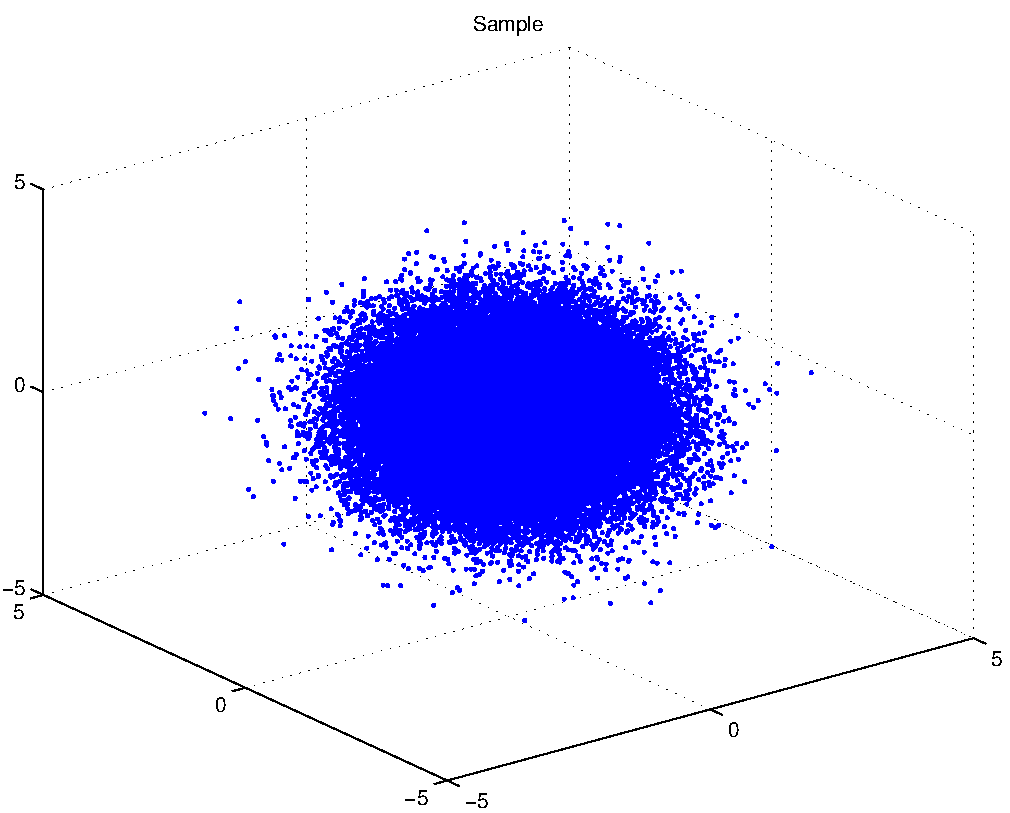
\includegraphics[width=10.0cm,height=10.0cm]{R_3_Normal.pdf}

Generate a sample from a unifom mixture of three Gaussians in $R^3$
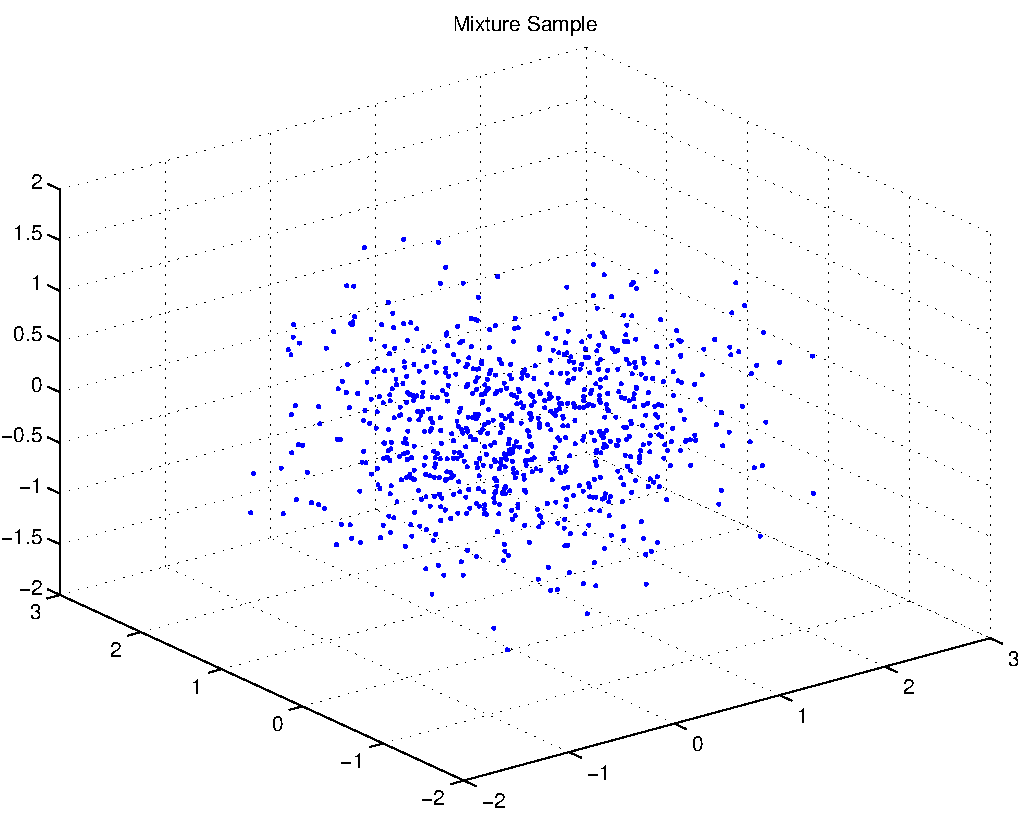
\includegraphics[width=10.0cm,height=10.0cm]{R_3_Normal_Mixture.pdf}

QueryPerformanceCounter  =  +15.872
\subsubsection{Matrix Multiply}
Comparing naive matrix multiply verus Intel MKL dgemm for matrix of size +2048.
This is for type double (hence the d in dgemm).
Naive type double matrix multiply tic toc  =  +0.370
dgemm plus row to column major transpose operation tic toc  =  +0.324
Comparing naive matrix multiply verus Intel MKL sgemm for matrix of size +2048.
This is for type float (hence the s in dgemm).
Naive type float matrix multiply tic toc  =  +0.296
sgemm plus row to column major transpose operation tic toc  =  +0.242
QueryPerformanceCounter  =  +1.376
\subsubsection{Descriptive Statistics}
Mean N(0,1): +0.003
Variance N(0,1): +1.006
Mean N(0,1) [recurrence relation method] :+0.003
Variance [recurrence relation method] :+1.006
Skewness : +0.007
Kurtosis : +2.997
QueryPerformanceCounter  =  +0.019
\subsubsection{Time Series }
+0.093
+0.726
+0.011
+2.178
QueryPerformanceCounter  =  +0.035
QueryPerformanceCounter  =  +6.150
\subsubsection{Iterated Exponential Filtering }
$\mu_1 =+0.093$
$\mu_2 =+0.726$
$\mu_3 =+0.011$
$\mu_4 =+2.178$
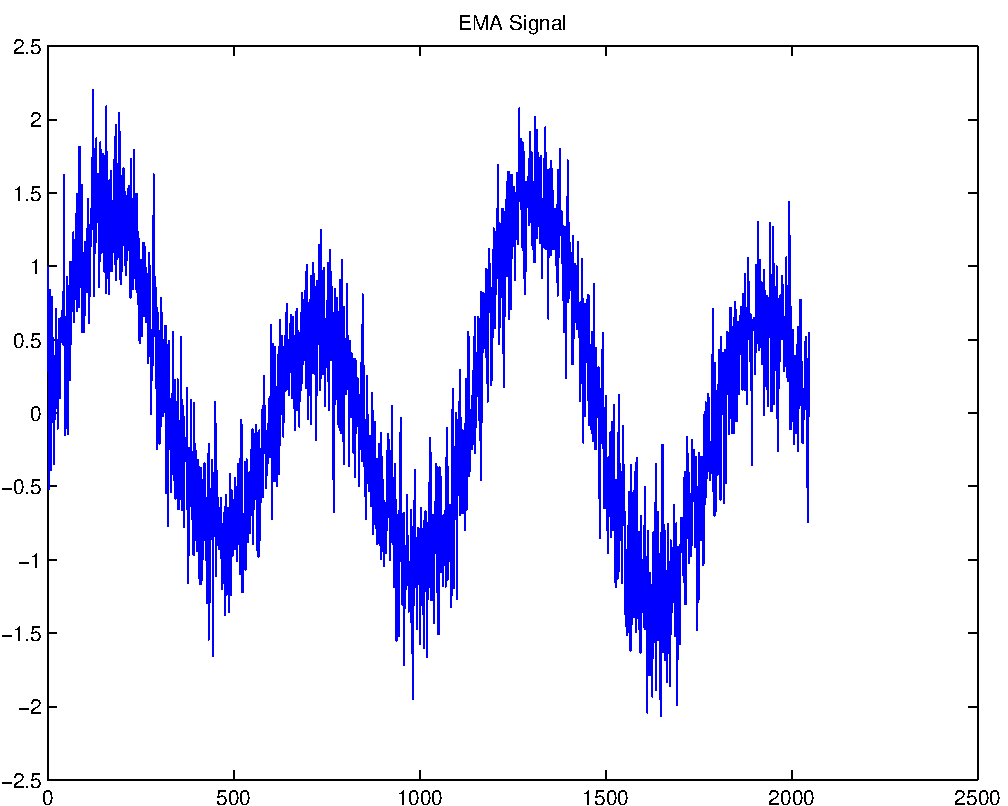
\includegraphics[width=10.0cm,height=10.0cm]{EMA_signal.pdf}

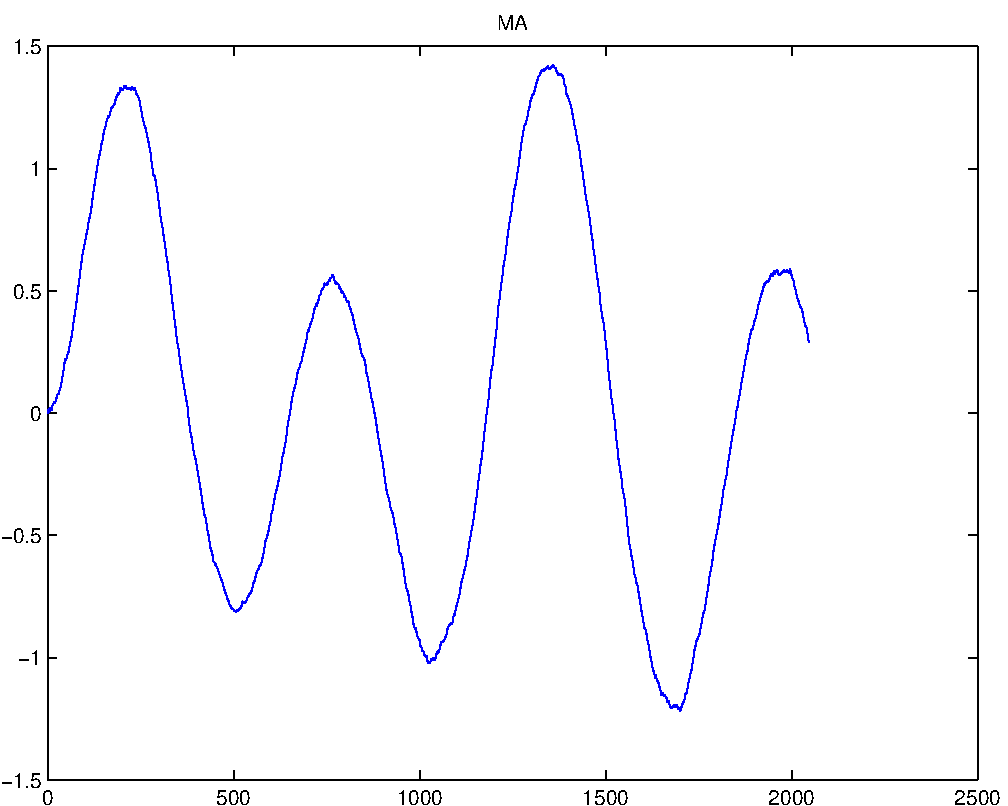
\includegraphics[width=10.0cm,height=10.0cm]{MA.pdf}

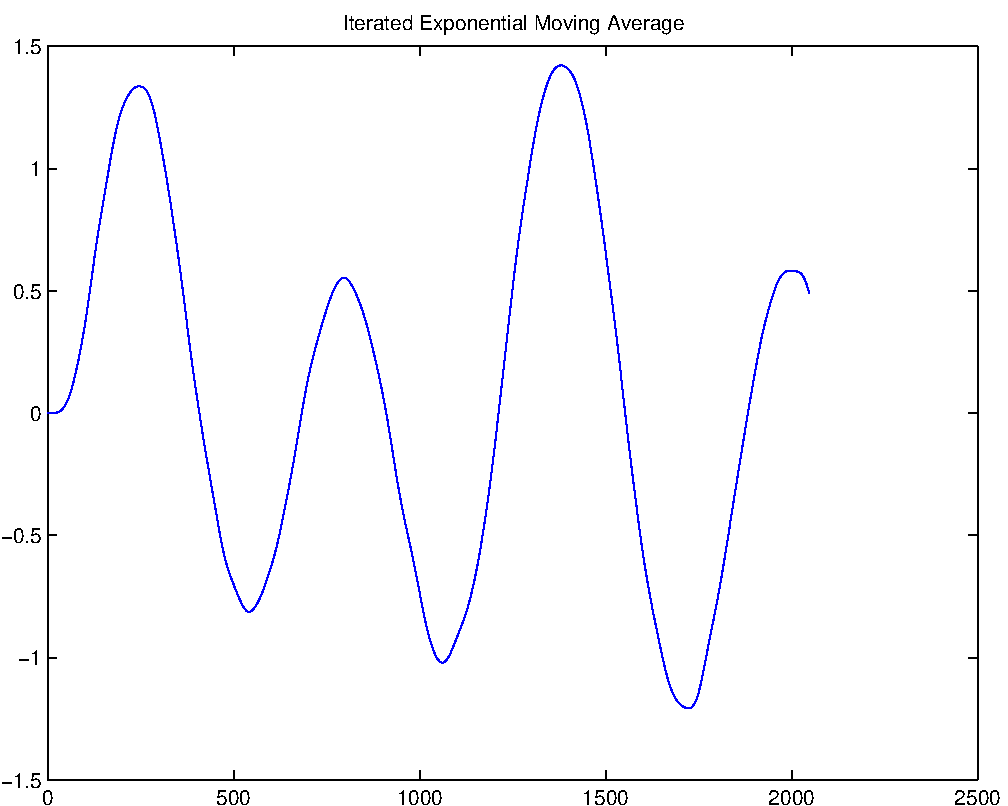
\includegraphics[width=10.0cm,height=10.0cm]{IEMA.pdf}

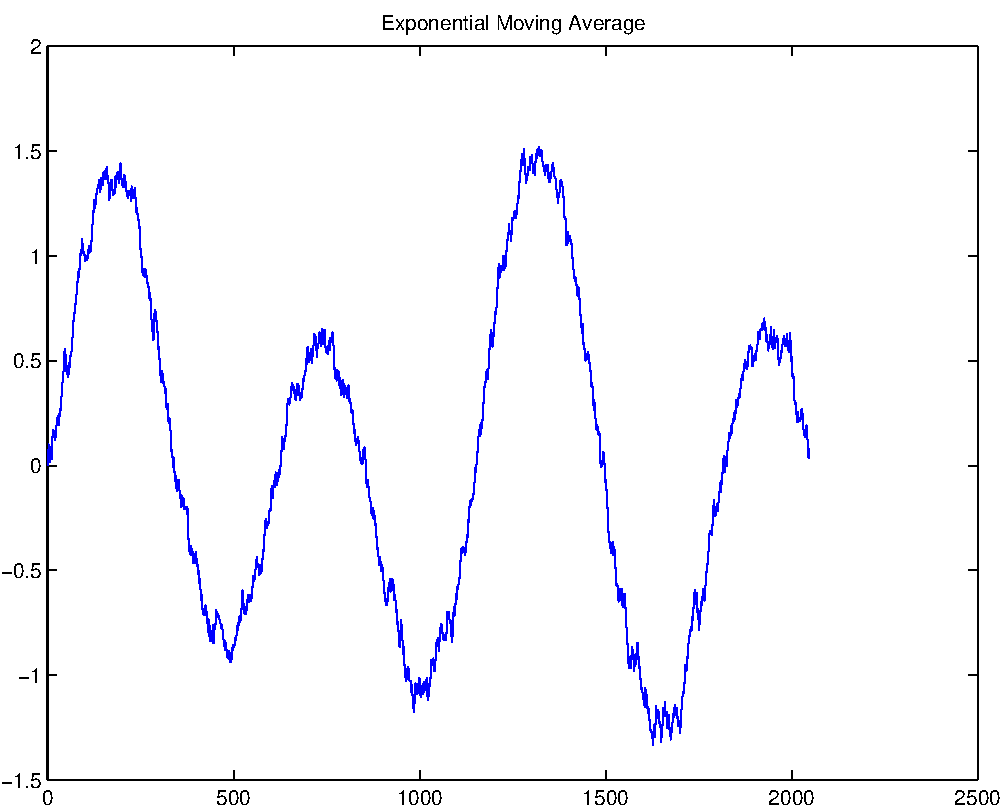
\includegraphics[width=10.0cm,height=10.0cm]{EMA.pdf}

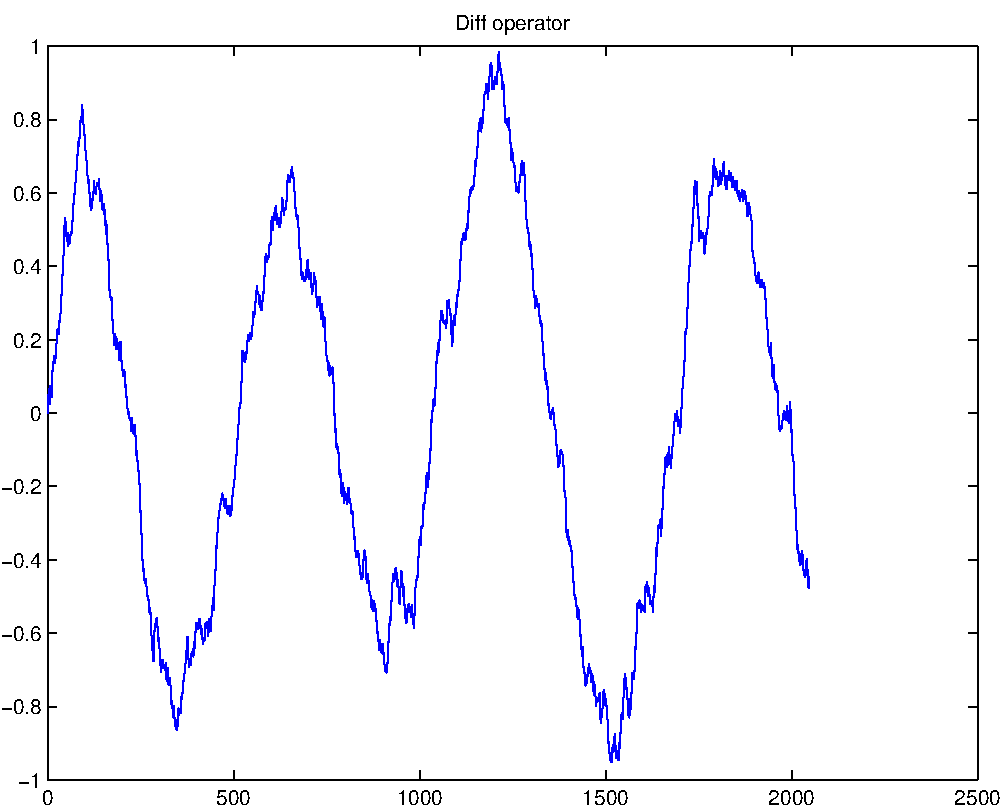
\includegraphics[width=10.0cm,height=10.0cm]{DIFF.pdf}

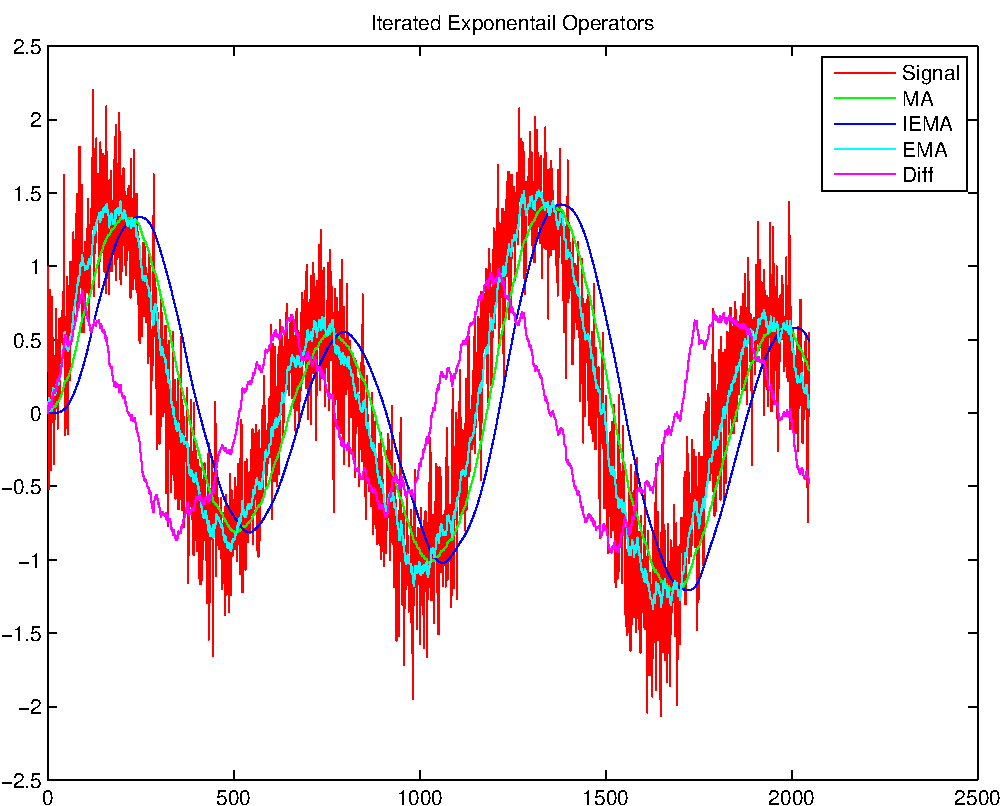
\includegraphics[width=10.0cm,height=10.0cm]{IteratedExponentailOperators.pdf}

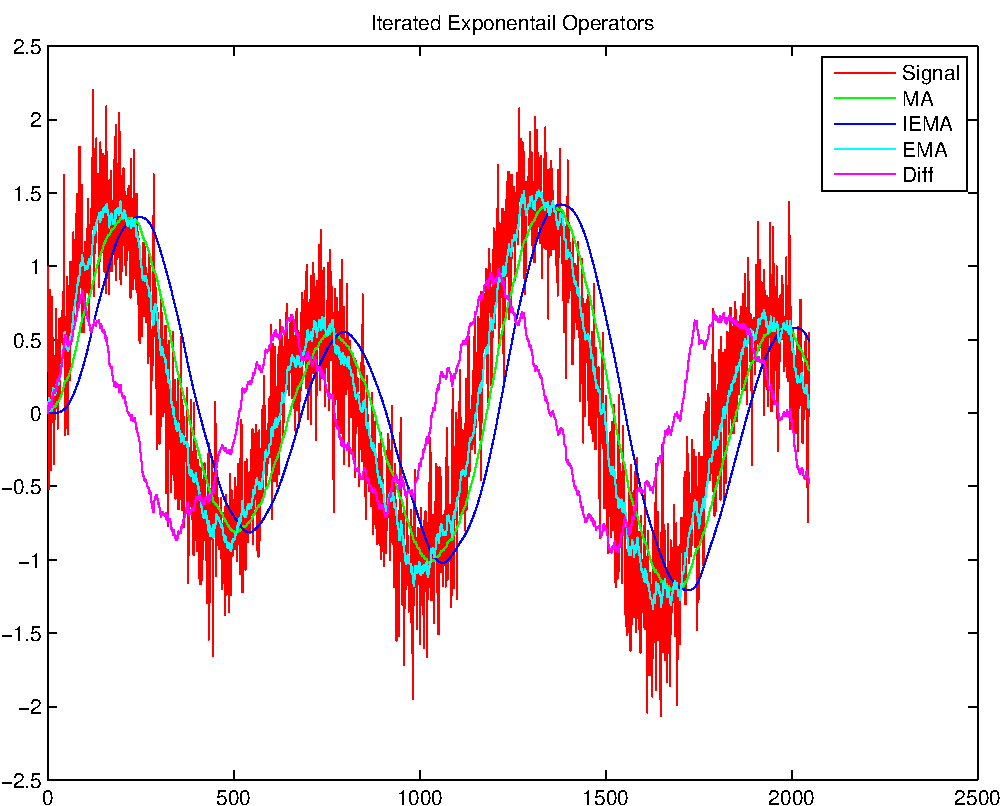
\includegraphics[width=10.0cm,height=10.0cm]{IteratedExponentailOperators.pdf}

QueryPerformanceCounter  =  +8.123
\subsubsection{Testing binary writer}
Binary writer Speedup 1GB Double Matrix +41.556

Binary reader Speedup 1GB Double Matrix +205.740

Binary writer Speedup 1GB Double vector +10.594

Binary reader Speedup 1GB Double Matrix +167.027

QueryPerformanceCounter  =  +0.908
\subsubsection{Testing Gaussian Mixture Point Cloud and Latex Plotting Capabilities.}
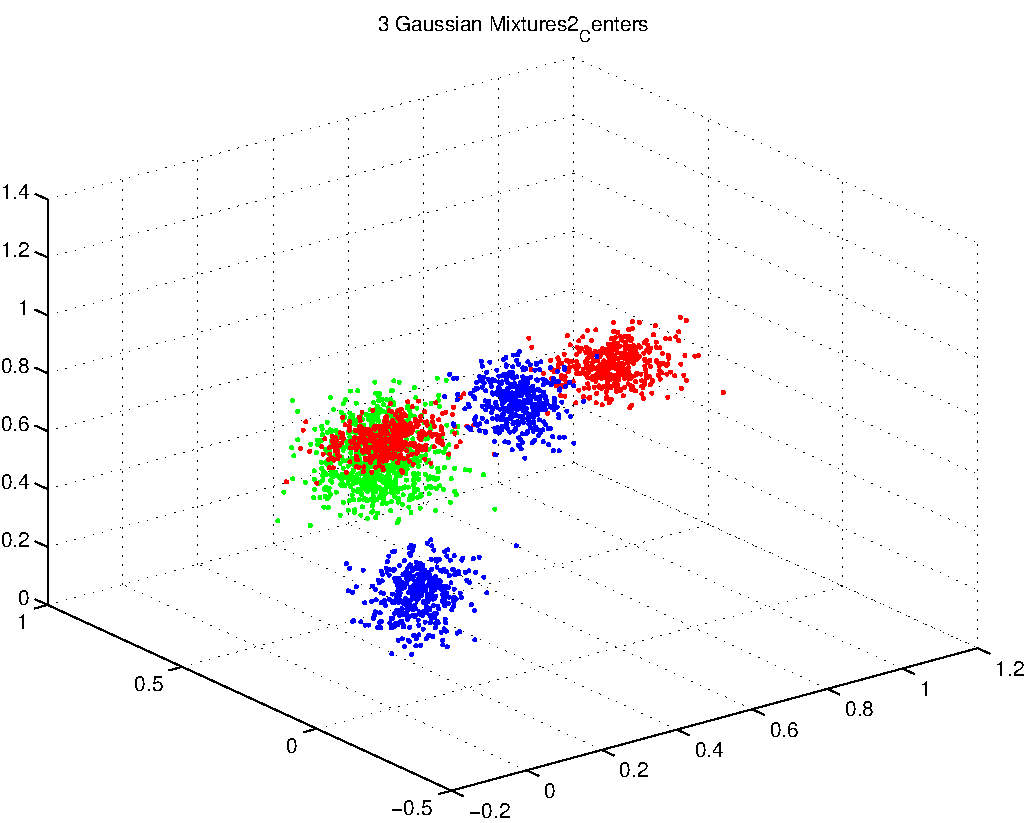
\includegraphics[width=10.0cm,height=10.0cm]{GaussianMixture_Dim_3_Centers2.pdf}

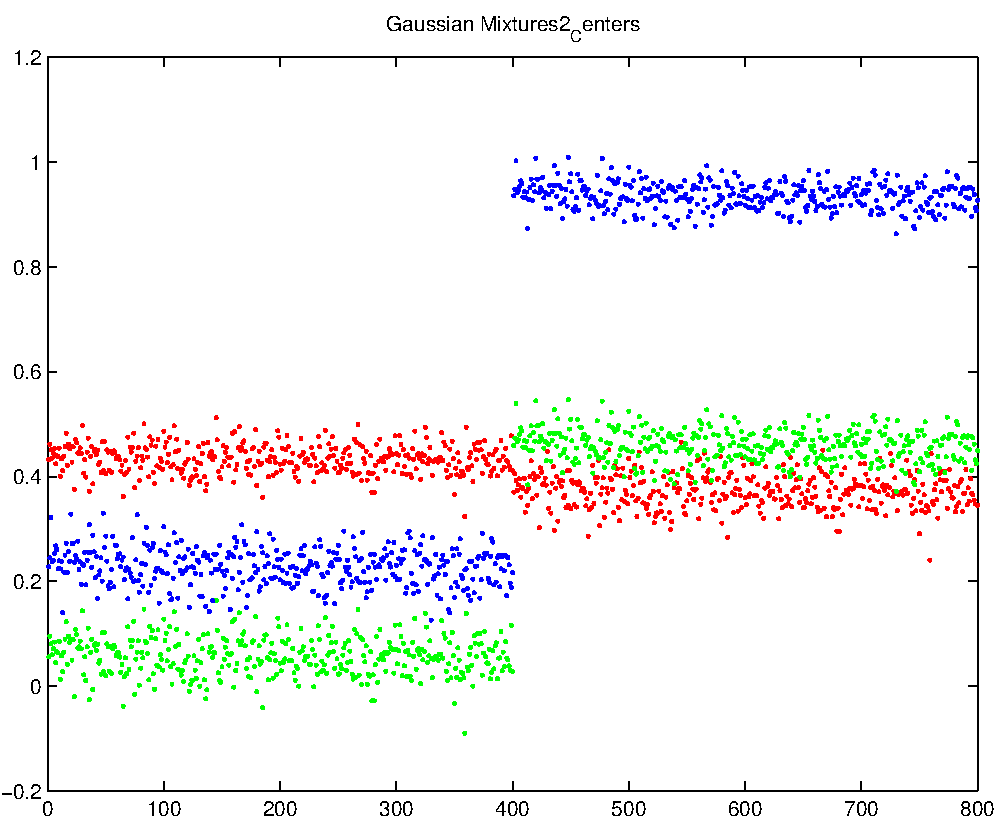
\includegraphics[width=10.0cm,height=10.0cm]{GaussianMixture_Dim_1_Centers2.pdf}

QueryPerformanceCounter  =  +2.799
\subsubsection{Intel VSL Function Check}
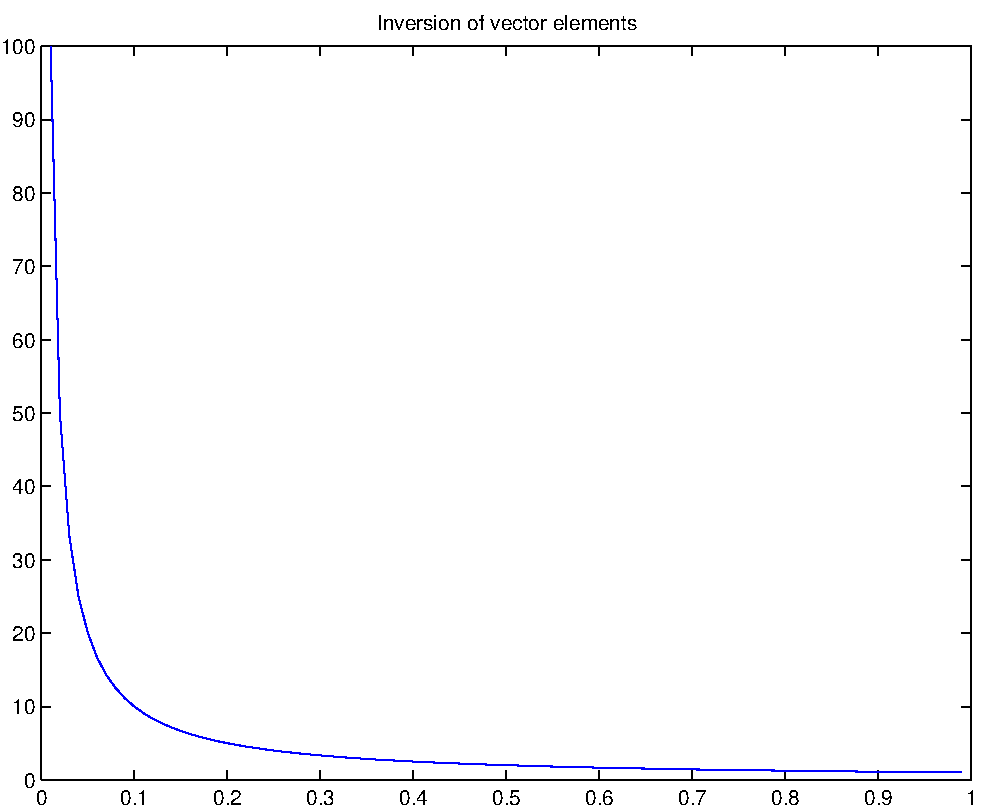
\includegraphics[width=10.0cm,height=10.0cm]{klVSLInv.pdf}

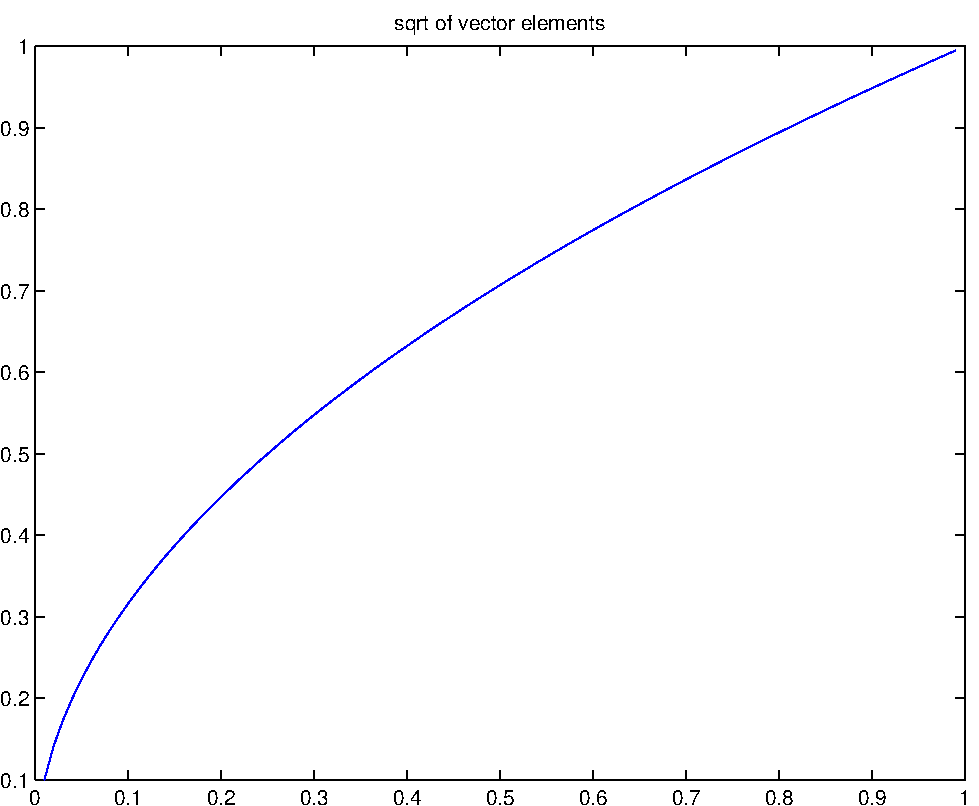
\includegraphics[width=10.0cm,height=10.0cm]{klVSLSqrt.pdf}

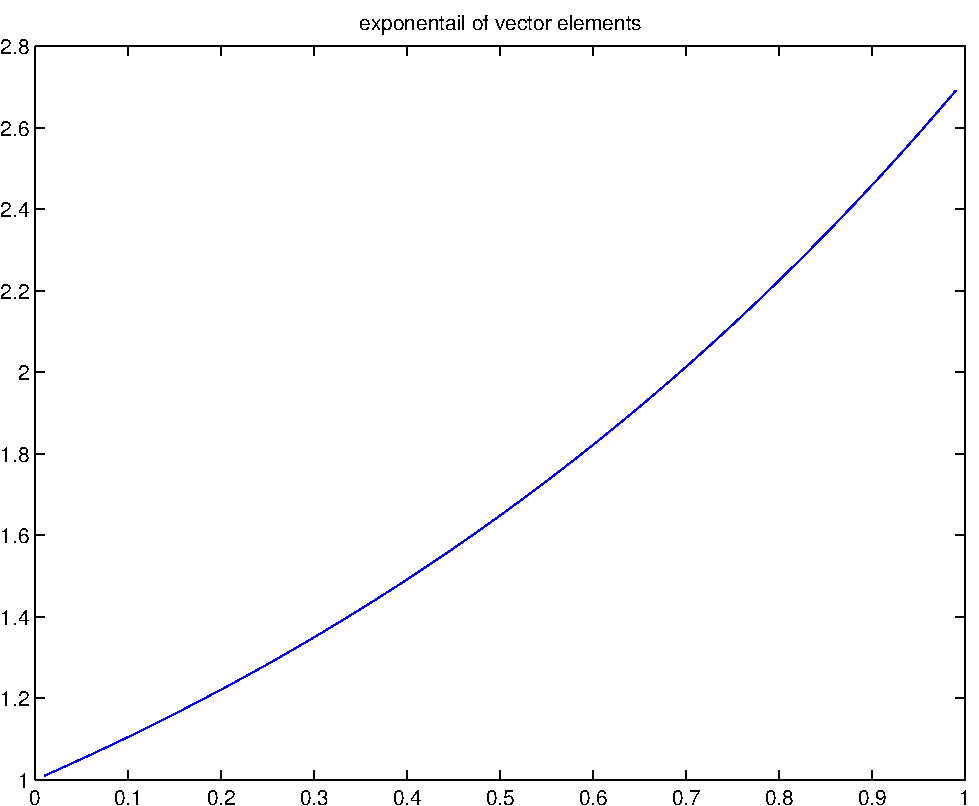
\includegraphics[width=10.0cm,height=10.0cm]{klVSLExp.pdf}

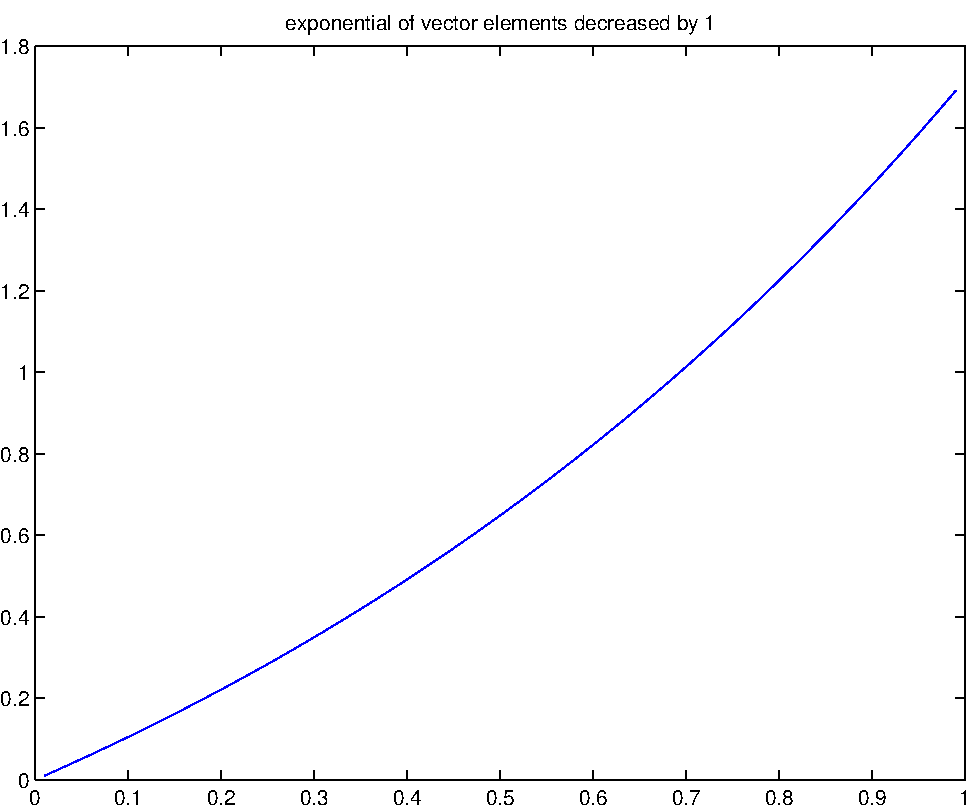
\includegraphics[width=10.0cm,height=10.0cm]{klVSLExpm1.pdf}

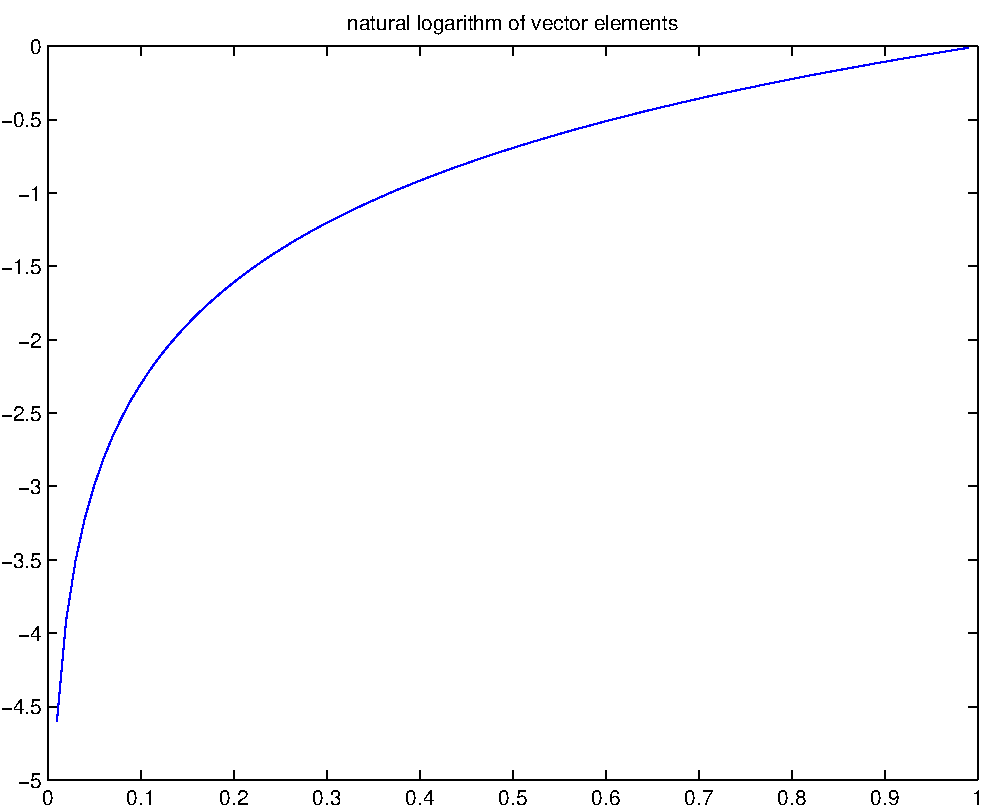
\includegraphics[width=10.0cm,height=10.0cm]{klVSLLn.pdf}

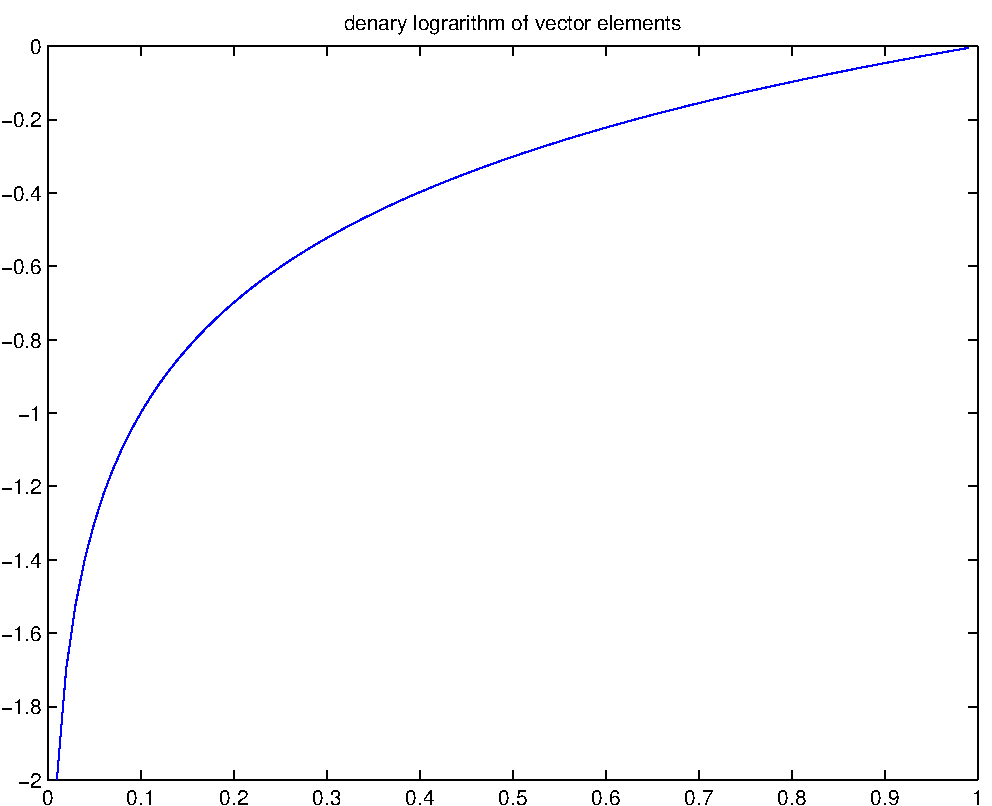
\includegraphics[width=10.0cm,height=10.0cm]{klVSLLog10.pdf}

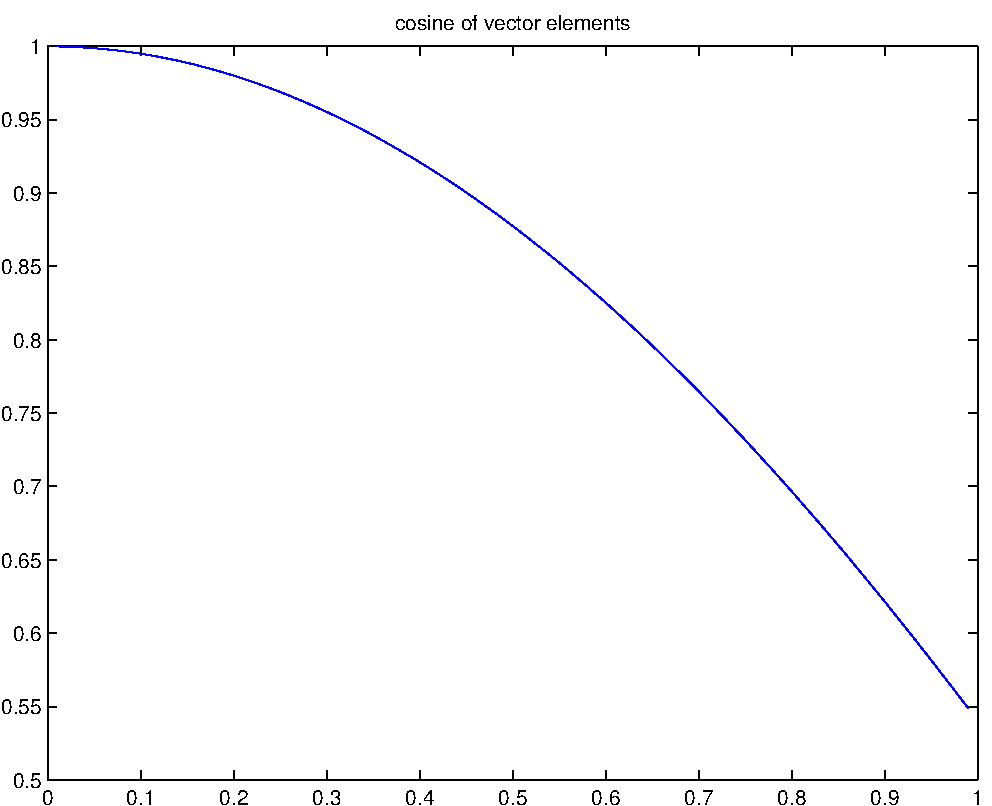
\includegraphics[width=10.0cm,height=10.0cm]{klVSLCos.pdf}

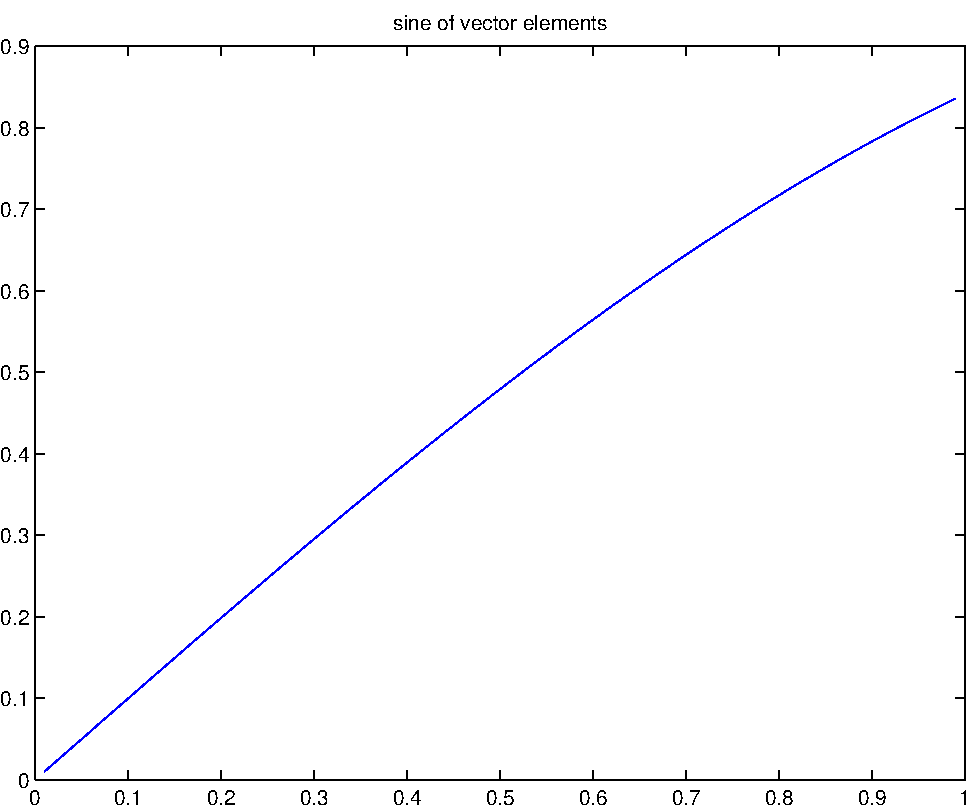
\includegraphics[width=10.0cm,height=10.0cm]{klVSLSin.pdf}

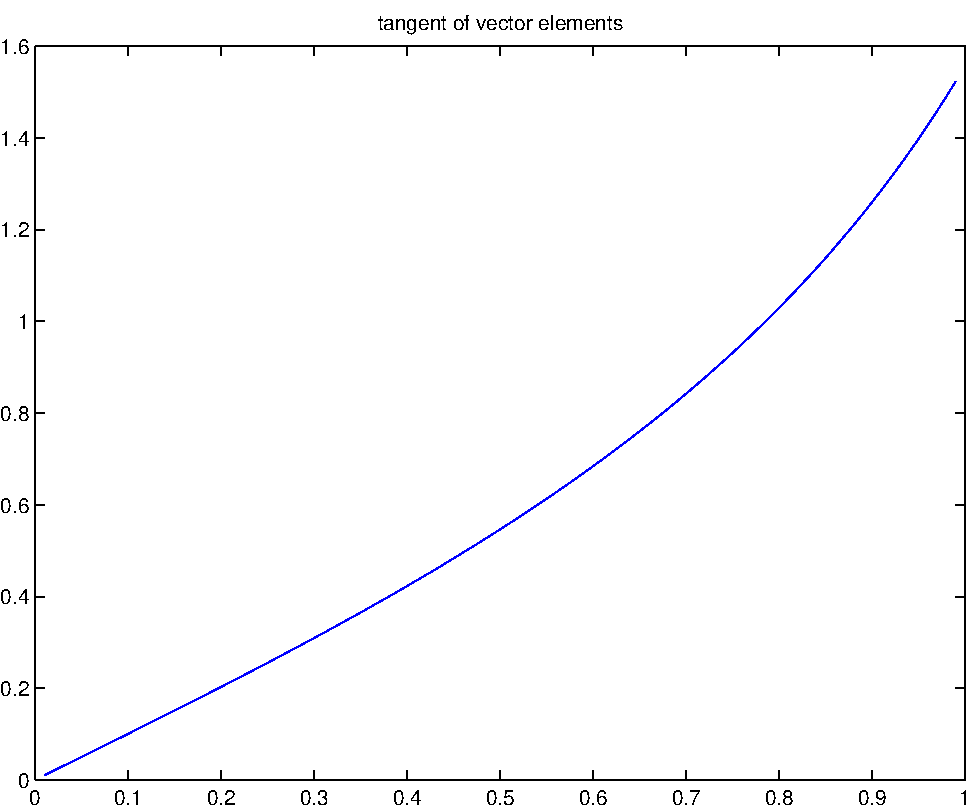
\includegraphics[width=10.0cm,height=10.0cm]{klVSLTan.pdf}

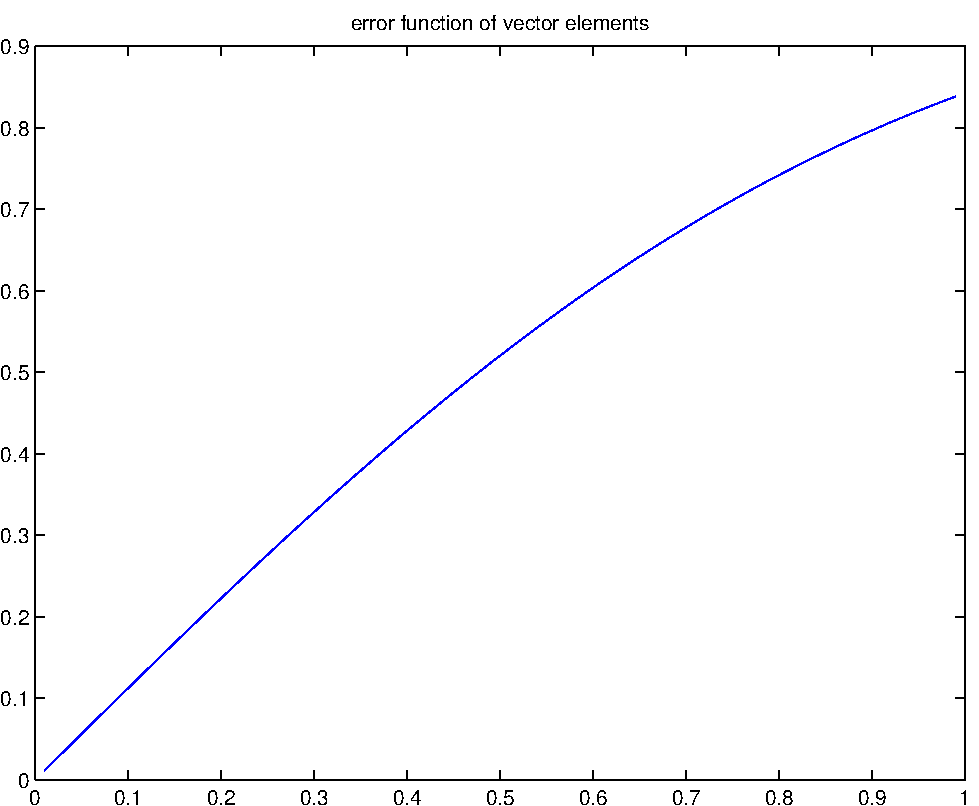
\includegraphics[width=10.0cm,height=10.0cm]{klVSLErf.pdf}

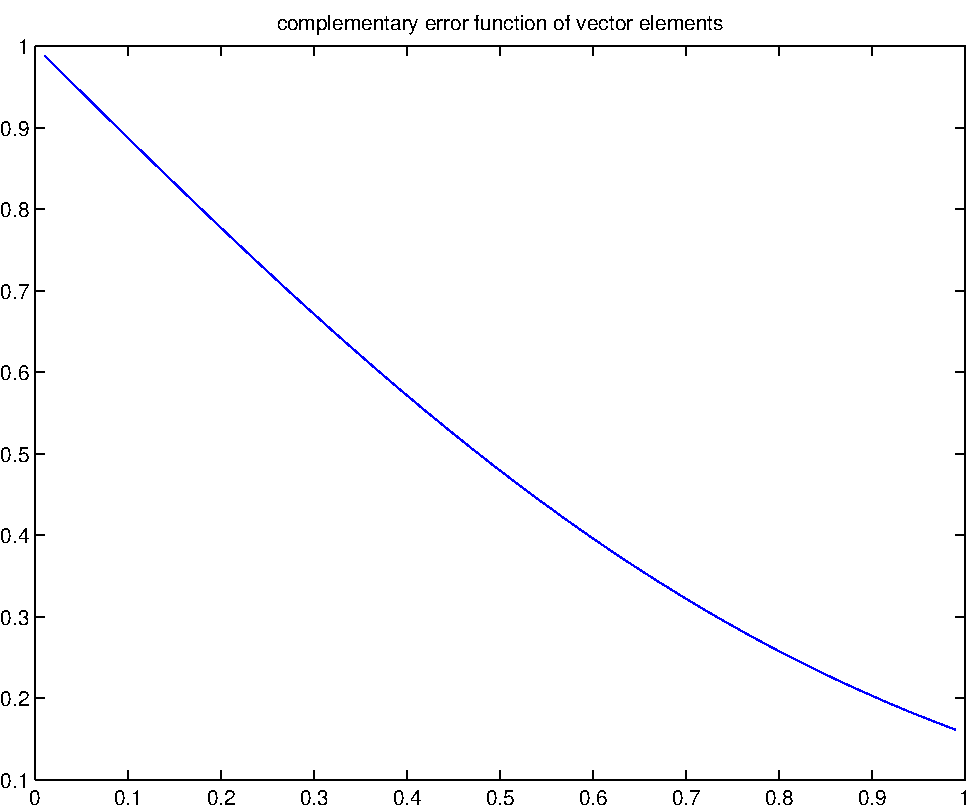
\includegraphics[width=10.0cm,height=10.0cm]{klVSLErfc.pdf}

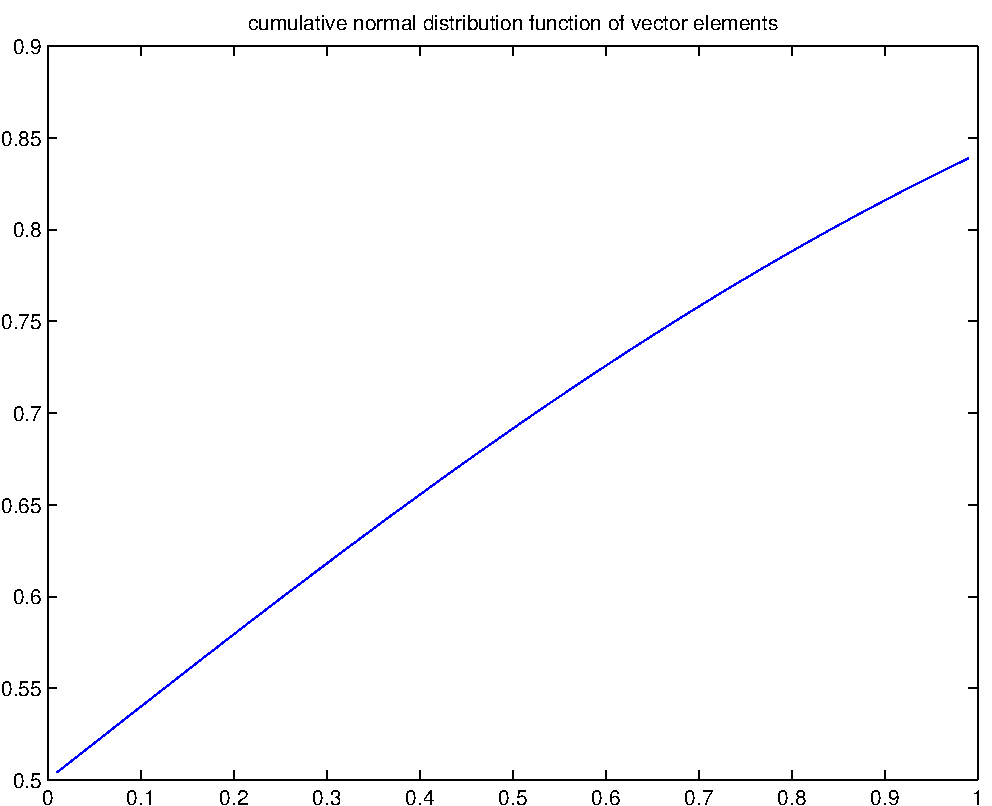
\includegraphics[width=10.0cm,height=10.0cm]{klVSLCdfNorm.pdf}

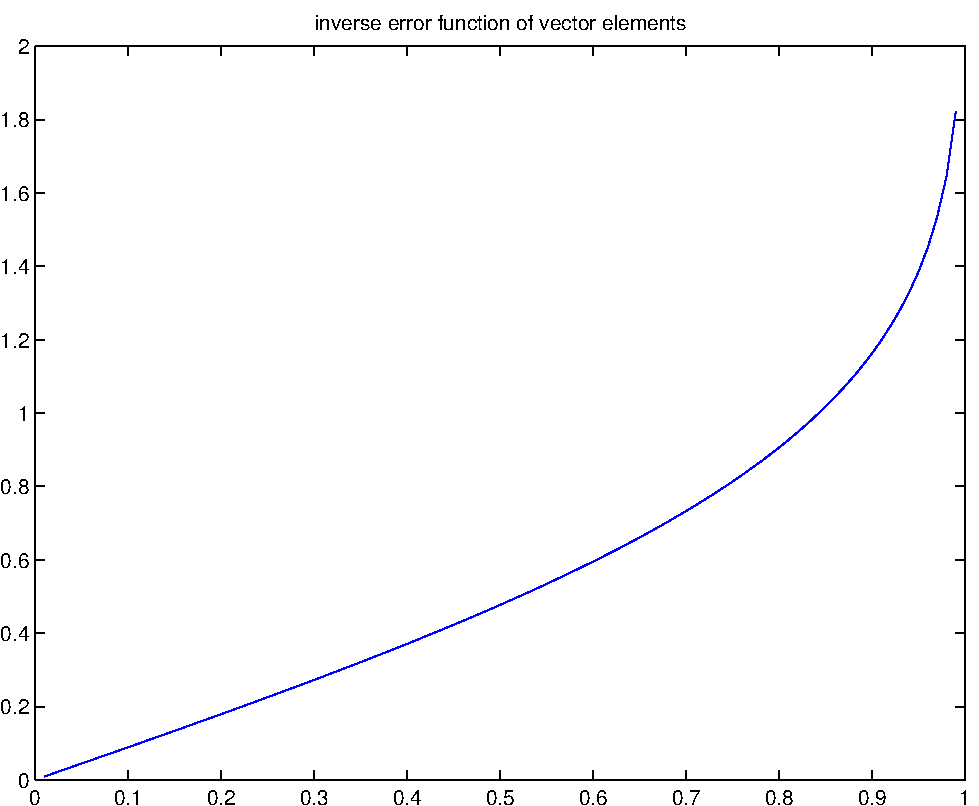
\includegraphics[width=10.0cm,height=10.0cm]{klVSLErfInv.pdf}

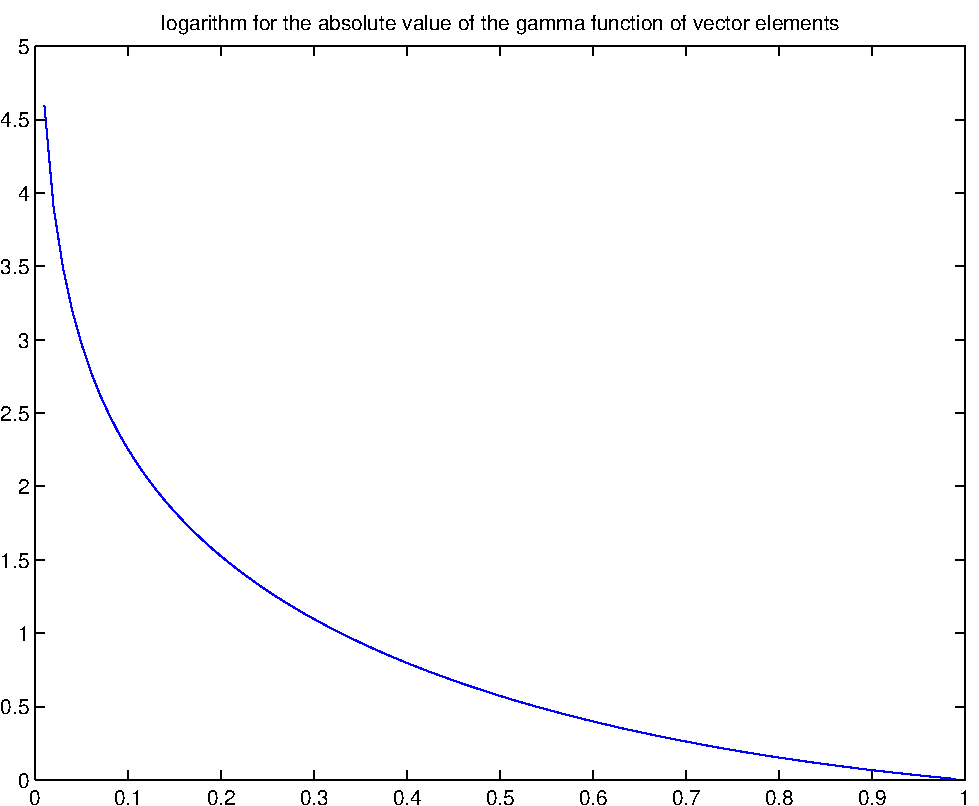
\includegraphics[width=10.0cm,height=10.0cm]{klVSLLGamma.pdf}

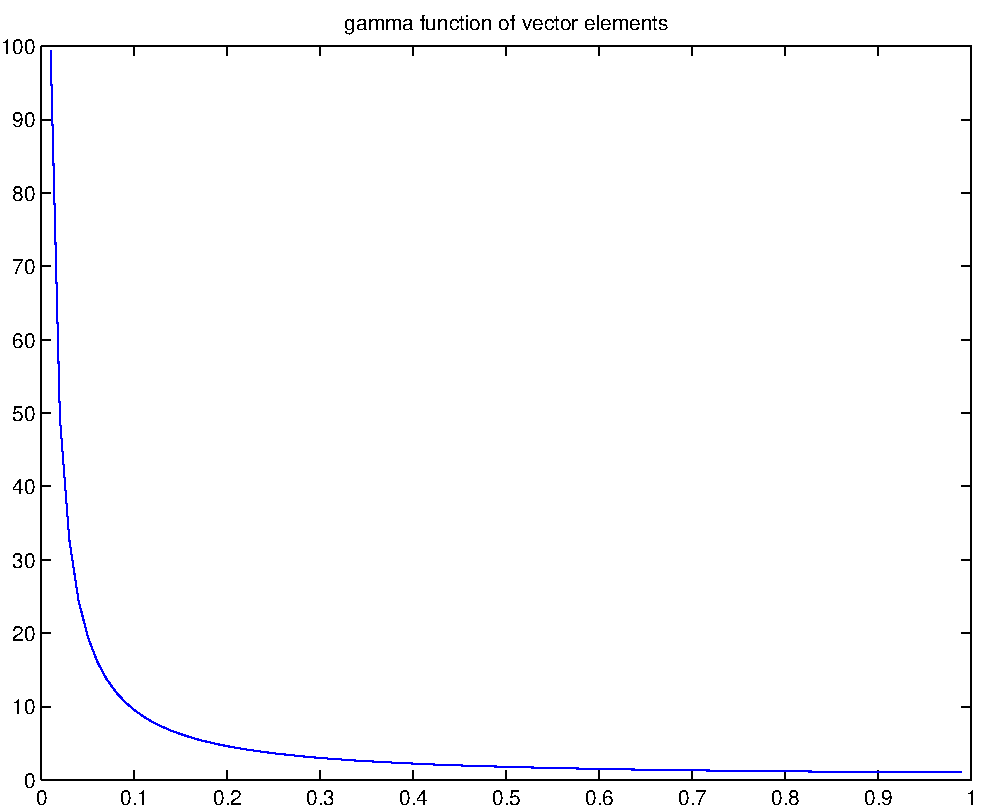
\includegraphics[width=10.0cm,height=10.0cm]{klVSLTGamma.pdf}

QueryPerformanceCounter  =  +15.275
\subsubsection{Gram Matrix Consistency Check}
Sample Size = 4096
Feature dim = 3

$$Sigma$ = \left(
\begin{array}{
ccc}
+1.140 & +1.535 & +0.581 \\
+1.535 & +9.988 & +1.605 \\
+0.581 & +1.605 & +0.428 \\
\end{array}
\right)$ \newline 

$Sample Covariance = \left(
\begin{array}{
ccc}
+1.150 & +1.644 & +0.596 \\
+1.644 & +10.296 & +1.693 \\
+0.596 & +1.693 & +0.442 \\
\end{array}
\right)$ \newline 

$Sample Mean = \left(
\begin{array}{
ccc}
+0.98980 & +1.00540 & +1.00216 \\
\end{array}
\right)$ \newline 

$Sample Covariance-$Omega$ = \left(
\begin{array}{
ccc}
+0.010 & +0.109 & +0.014 \\
+0.109 & +0.307 & +0.088 \\
+0.014 & +0.088 & +0.015 \\
\end{array}
\right)$ \newline 

$Sample Covariance Eigs = \left(
\begin{array}{
ccc}
(+10.88264,+0.00000) & (+0.96643,+0.00000) & (+0.03867,+0.00000) \\
\end{array}
\right)$ \newline 

$Centered Mean = \left(
\begin{array}{
ccc}
-0.00000 & -0.00000 & +0.00000 \\
\end{array}
\right)$ \newline 

$Centered Covariance = \left(
\begin{array}{
ccc}
+1.150 & +1.644 & +0.596 \\
+1.644 & +10.296 & +1.693 \\
+0.596 & +1.693 & +0.442 \\
\end{array}
\right)$ \newline 

$Gram Matrix Gf Not scaled by sample size = \left(
\begin{array}{
ccc}
+4709.185 & +6731.676 & +2439.704 \\
+6731.676 & +42171.067 & +6934.030 \\
+2439.704 & +6934.030 & +1811.956 \\
\end{array}
\right)$ \newline 

$Gram Matrix Gf  scaled by sample size = \left(
\begin{array}{
ccc}
+1.150 & +1.643 & +0.596 \\
+1.643 & +10.296 & +1.693 \\
+0.596 & +1.693 & +0.442 \\
\end{array}
\right)$ \newline 

$SampleCovariance - Scaled Gf = \left(
\begin{array}{
ccc}
+0.000 & +0.000 & +0.000 \\
+0.000 & +0.003 & +0.000 \\
+0.000 & +0.000 & +0.000 \\
\end{array}
\right)$ \newline 

$EigenDecomp of SampleCovariance = \left(
\begin{array}{
ccc}
-0.174 & -0.970 & -0.167 \\
+0.918 & -0.221 & +0.328 \\
-0.356 & -0.096 & +0.930 \\
\end{array}
\right)$ \newline 

$EigenDecomp of Gram Matrix = \left(
\begin{array}{
ccc}
-0.128 & -0.973 & -0.193 \\
-0.352 & +0.227 & -0.908 \\
+0.927 & -0.048 & -0.371 \\
\end{array}
\right)$ \newline 

QueryPerformanceCounter  =  +1.290
\subsubsection{Eigen Solver Checks}
\subsubsection{Haar Distributed Random Orthogonal Matrix $A \in O(n)$}
 Testing Operator Norm
Number of Dimensions: +8

$A = \left(
\begin{array}{
cccccccc}
-0.483 & -0.628 & +0.223 & +0.431 & -0.184 & -0.270 & +0.094 & -0.146 \\
+0.452 & -0.157 & +0.386 & +0.046 & +0.552 & -0.535 & -0.109 & +0.132 \\
+0.317 & +0.132 & +0.211 & +0.477 & +0.159 & +0.378 & +0.306 & -0.590 \\
+0.073 & +0.258 & +0.693 & +0.132 & -0.444 & +0.137 & +0.073 & +0.457 \\
-0.334 & +0.605 & +0.161 & -0.103 & -0.080 & -0.547 & +0.036 & -0.423 \\
-0.272 & +0.306 & -0.281 & +0.478 & +0.370 & -0.064 & +0.398 & +0.474 \\
+0.401 & -0.134 & -0.229 & -0.154 & -0.390 & -0.340 & +0.691 & +0.015 \\
+0.333 & +0.139 & -0.345 & +0.551 & -0.378 & -0.246 & -0.493 & +0.017 \\
\end{array}
\right)$ \newline 

$Det(A) :   A \in O(n)$ = (-1.000,+0.000)

$L = \left(
\begin{array}{
cccccccc}
+1.000 & +0.000 & +0.000 & +0.000 & +0.000 & +0.000 & +0.000 & +0.000 \\
+0.691 & +1.000 & +0.000 & +0.000 & +0.000 & +0.000 & +0.000 & +0.000 \\
-0.150 & +0.157 & +1.000 & +0.000 & +0.000 & +0.000 & +0.000 & +0.000 \\
-0.690 & -0.283 & -0.260 & +1.000 & +0.000 & +0.000 & +0.000 & +0.000 \\
-0.937 & -0.717 & +0.826 & -0.066 & +1.000 & +0.000 & +0.000 & +0.000 \\
+0.564 & +0.635 & -0.567 & +0.795 & +0.862 & +1.000 & +0.000 & +0.000 \\
-0.830 & -0.631 & -0.054 & -0.044 & -0.737 & -0.922 & +1.000 & +0.000 \\
-0.657 & -0.270 & +0.495 & +0.652 & +0.898 & +0.780 & +0.026 & +1.000 \\
\end{array}
\right)$ \newline 

$U = \left(
\begin{array}{
cccccccc}
-0.483 & -0.628 & +0.223 & +0.431 & -0.184 & -0.270 & +0.094 & -0.146 \\
+0.000 & +1.040 & +0.007 & -0.401 & +0.047 & -0.360 & -0.028 & -0.322 \\
+0.000 & +0.000 & +0.726 & +0.260 & -0.479 & +0.152 & +0.092 & +0.486 \\
+0.000 & +0.000 & +0.000 & +0.803 & -0.617 & -0.495 & -0.413 & -0.048 \\
+0.000 & +0.000 & +0.000 & +0.000 & +0.768 & -1.205 & -0.145 & -0.641 \\
+0.000 & +0.000 & +0.000 & +0.000 & +0.000 & +1.835 & +0.868 & +1.627 \\
+0.000 & +0.000 & +0.000 & +0.000 & +0.000 & +0.000 & +1.431 & +0.744 \\
+0.000 & +0.000 & +0.000 & +0.000 & +0.000 & +0.000 & +0.000 & -1.695 \\
\end{array}
\right)$ \newline 

$L * U  = \left(
\begin{array}{
cccccccc}
-0.483 & -0.628 & +0.223 & +0.431 & -0.184 & -0.270 & +0.094 & -0.146 \\
-0.334 & +0.605 & +0.161 & -0.103 & -0.080 & -0.547 & +0.036 & -0.423 \\
+0.073 & +0.258 & +0.693 & +0.132 & -0.444 & +0.137 & +0.073 & +0.457 \\
+0.333 & +0.139 & -0.345 & +0.551 & -0.378 & -0.246 & -0.493 & +0.017 \\
+0.452 & -0.157 & +0.386 & +0.046 & +0.552 & -0.535 & -0.109 & +0.132 \\
-0.272 & +0.306 & -0.281 & +0.478 & +0.370 & -0.064 & +0.398 & +0.474 \\
+0.401 & -0.134 & -0.229 & -0.154 & -0.390 & -0.340 & +0.691 & +0.015 \\
+0.317 & +0.132 & +0.211 & +0.477 & +0.159 & +0.378 & +0.306 & -0.590 \\
\end{array}
\right)$ \newline 

$Det(L) :    = (+1.000,+0.000)     Det(U) :    = (+1.000,+0.000)     Det(LU) :    = (+1.000,+0.000)$

$||A||_{L_1}$  = +2.664

$||A||_{L_{\infty}}$ = +2.644

$||A^{-1}||_{L_1}$  = +2.644

$||A^{-1}||_{L_{\infty}}$ = +2.664

$||A||_{L_{\infty}} * ||A^{-1}||_{L_{\infty}} = +7.043$

$||A||_{L_1} * ||A^{-1}||_{L_1} = +7.043$

Frobenious Norm  $||A||_{\textit{F}}$ via $\sum\limits_{i,j =0}^{n} \|A_{i,j}|$   of  $A \in O(n)$  +2.828

$L_1$ condition number of Haar Distributed Random Orthogonal Matrix $A \in O(n)$ +6.846

$A = \left(
\begin{array}{
cccccccc}
-0.483 & -0.628 & +0.223 & +0.431 & -0.184 & -0.270 & +0.094 & -0.146 \\
+0.452 & -0.157 & +0.386 & +0.046 & +0.552 & -0.535 & -0.109 & +0.132 \\
+0.317 & +0.132 & +0.211 & +0.477 & +0.159 & +0.378 & +0.306 & -0.590 \\
+0.073 & +0.258 & +0.693 & +0.132 & -0.444 & +0.137 & +0.073 & +0.457 \\
-0.334 & +0.605 & +0.161 & -0.103 & -0.080 & -0.547 & +0.036 & -0.423 \\
-0.272 & +0.306 & -0.281 & +0.478 & +0.370 & -0.064 & +0.398 & +0.474 \\
+0.401 & -0.134 & -0.229 & -0.154 & -0.390 & -0.340 & +0.691 & +0.015 \\
+0.333 & +0.139 & -0.345 & +0.551 & -0.378 & -0.246 & -0.493 & +0.017 \\
\end{array}
\right)$ \newline 

$L_{\infty}$ condition number of Haar Distributed Random Orthogonal Matrix $A \in O(n)$ +6.764

Eigenvalues of $A \in O(n)$

(-0.836,+0.549), (-0.836,-0.549), (-1.000,+0.000), (+0.068,+0.998), (+0.068,-0.998), (+0.901,+0.433), (+0.901,-0.433), (+1.000,+0.000)

 $|\lambda | : \lambda \in \sigma(A) , A \in O(n)$

+1.000, +1.000, +1.000, +1.000, +1.000, +1.000, +1.000, +1.000


Calculating $A^{\dag} A,$  we expect $A^{\dag} A \approx I$

$A^{\dag} A = \left(
\begin{array}{
cccccccc}
+1.000 & +0.000 & -0.000 & +0.000 & +0.000 & +0.000 & -0.000 & +0.000 \\
+0.000 & +1.000 & +0.000 & -0.000 & -0.000 & -0.000 & +0.000 & -0.000 \\
-0.000 & +0.000 & +1.000 & +0.000 & -0.000 & -0.000 & -0.000 & -0.000 \\
+0.000 & -0.000 & +0.000 & +1.000 & -0.000 & +0.000 & +0.000 & +0.000 \\
+0.000 & -0.000 & -0.000 & -0.000 & +1.000 & +0.000 & +0.000 & +0.000 \\
+0.000 & -0.000 & -0.000 & +0.000 & +0.000 & +1.000 & +0.000 & +0.000 \\
-0.000 & +0.000 & -0.000 & +0.000 & +0.000 & +0.000 & +1.000 & +0.000 \\
+0.000 & -0.000 & -0.000 & +0.000 & +0.000 & +0.000 & +0.000 & +1.000 \\
\end{array}
\right)$ \newline 

Calculating $A^{-1} ,  A \in O(n)$.

$A^{-1} = \left(
\begin{array}{
cccccccc}
-0.483 & +0.452 & +0.317 & +0.073 & -0.334 & -0.272 & +0.401 & +0.333 \\
-0.628 & -0.157 & +0.132 & +0.258 & +0.605 & +0.306 & -0.134 & +0.139 \\
+0.223 & +0.386 & +0.211 & +0.693 & +0.161 & -0.281 & -0.229 & -0.345 \\
+0.431 & +0.046 & +0.477 & +0.132 & -0.103 & +0.478 & -0.154 & +0.551 \\
-0.184 & +0.552 & +0.159 & -0.444 & -0.080 & +0.370 & -0.390 & -0.378 \\
-0.270 & -0.535 & +0.378 & +0.137 & -0.547 & -0.064 & -0.340 & -0.246 \\
+0.094 & -0.109 & +0.306 & +0.073 & +0.036 & +0.398 & +0.691 & -0.493 \\
-0.146 & +0.132 & -0.590 & +0.457 & -0.423 & +0.474 & +0.015 & +0.017 \\
\end{array}
\right)$ \newline 

Calculating $A^{-1} *A  ,  A \in O(n)$.   We expect $A^{-1} *A  \approx I$. 

$A^{-1} *A = \left(
\begin{array}{
cccccccc}
+1.000 & -0.000 & +0.000 & -0.000 & +0.000 & -0.000 & -0.000 & -0.000 \\
+0.000 & +1.000 & -0.000 & +0.000 & +0.000 & +0.000 & +0.000 & +0.000 \\
+0.000 & -0.000 & +1.000 & -0.000 & -0.000 & -0.000 & +0.000 & +0.000 \\
-0.000 & +0.000 & -0.000 & +1.000 & +0.000 & -0.000 & +0.000 & -0.000 \\
+0.000 & +0.000 & +0.000 & +0.000 & +1.000 & -0.000 & +0.000 & -0.000 \\
-0.000 & -0.000 & +0.000 & +0.000 & -0.000 & +1.000 & +0.000 & +0.000 \\
+0.000 & -0.000 & -0.000 & -0.000 & +0.000 & +0.000 & +1.000 & -0.000 \\
+0.000 & -0.000 & +0.000 & +0.000 & -0.000 & -0.000 & -0.000 & +1.000 \\
\end{array}
\right)$ \newline 

Calculating SVD of  $A \in O(n)$

$U = \left(
\begin{array}{
cccccccc}
+0.255 & +0.182 & -0.133 & +0.226 & -0.413 & -0.532 & +0.301 & +0.537 \\
-0.483 & -0.628 & +0.223 & +0.431 & -0.184 & -0.270 & +0.094 & -0.146 \\
-0.195 & -0.040 & +0.549 & -0.340 & -0.253 & +0.090 & -0.440 & +0.526 \\
+0.158 & -0.551 & -0.425 & -0.616 & -0.095 & -0.295 & -0.120 & -0.033 \\
+0.171 & -0.297 & +0.088 & -0.123 & -0.310 & +0.615 & +0.608 & +0.125 \\
+0.069 & +0.290 & +0.293 & -0.240 & -0.586 & -0.187 & +0.049 & -0.621 \\
-0.055 & +0.012 & -0.500 & +0.320 & -0.528 & +0.367 & -0.480 & -0.010 \\
+0.776 & -0.308 & +0.326 & +0.305 & +0.060 & -0.003 & -0.300 & -0.101 \\
\end{array}
\right)$ \newline 

$S = \left(
\begin{array}{
cccccccc}
+1.000 & +0.000 & +0.000 & +0.000 & +0.000 & +0.000 & +0.000 & +0.000 \\
+0.000 & +1.000 & +0.000 & +0.000 & +0.000 & +0.000 & +0.000 & +0.000 \\
+0.000 & +0.000 & +1.000 & +0.000 & +0.000 & +0.000 & +0.000 & +0.000 \\
+0.000 & +0.000 & +0.000 & +1.000 & +0.000 & +0.000 & +0.000 & +0.000 \\
+0.000 & +0.000 & +0.000 & +0.000 & +1.000 & +0.000 & +0.000 & +0.000 \\
+0.000 & +0.000 & +0.000 & +0.000 & +0.000 & +1.000 & +0.000 & +0.000 \\
+0.000 & +0.000 & +0.000 & +0.000 & +0.000 & +0.000 & +1.000 & +0.000 \\
+0.000 & +0.000 & +0.000 & +0.000 & +0.000 & +0.000 & +0.000 & +1.000 \\
\end{array}
\right)$ \newline 

$V = \left(
\begin{array}{
cccccccc}
-0.000 & +1.000 & +0.000 & -0.000 & -0.000 & -0.000 & -0.000 & -0.000 \\
+0.140 & +0.000 & +0.044 & +0.079 & -0.398 & -0.223 & -0.642 & +0.593 \\
-0.307 & +0.000 & -0.565 & -0.550 & +0.271 & +0.225 & -0.055 & +0.396 \\
+0.381 & +0.000 & +0.644 & -0.529 & +0.303 & +0.206 & -0.060 & +0.148 \\
+0.088 & +0.000 & -0.103 & -0.212 & -0.552 & +0.639 & -0.259 & -0.396 \\
+0.387 & +0.000 & -0.301 & -0.466 & -0.074 & -0.608 & -0.102 & -0.396 \\
+0.632 & +0.000 & -0.374 & +0.383 & +0.441 & +0.276 & -0.209 & +0.000 \\
+0.429 & +0.000 & -0.147 & -0.049 & -0.414 & +0.063 & +0.678 & +0.396 \\
\end{array}
\right)$ \newline 

$U S V = \left(
\begin{array}{
cccccccc}
+0.330 & +0.255 & +0.240 & +0.393 & +0.138 & +0.152 & +0.340 & +0.675 \\
-0.117 & -0.483 & +0.211 & -0.192 & +0.664 & +0.342 & +0.322 & -0.098 \\
-0.344 & -0.195 & -0.445 & -0.309 & -0.217 & -0.241 & +0.522 & +0.416 \\
-0.394 & +0.158 & -0.032 & +0.629 & -0.048 & -0.017 & +0.471 & -0.445 \\
+0.533 & +0.171 & -0.542 & -0.001 & +0.446 & -0.335 & +0.168 & -0.232 \\
-0.500 & +0.069 & -0.117 & +0.250 & +0.508 & -0.335 & -0.449 & +0.313 \\
+0.065 & -0.055 & +0.614 & -0.137 & +0.014 & -0.743 & +0.194 & -0.083 \\
-0.255 & +0.776 & +0.120 & -0.486 & +0.181 & +0.157 & +0.141 & -0.071 \\
\end{array}
\right)$ \newline 

Calculating first few eigenvectors of $A \in O(n)$ using LAPACK syevx

\subsubsection{Wishart Matrix $A \in W(n)$}
$L_1$ condition number of Wishart Matrix +1489.694
$L_infty$ condition number of Wishart Matrix +1489.694
\subsubsection{Gaussian Orthogonal Ensemble $A \in GOE(n)$}
$L_1$ condition number of GOE Matrix +66.900
$L_\infty$ condition number of GOE Matrix +66.900
\subsubsection{The Identity Matrix $I \in M(n)$}
$L_1$ condition number of $I$ = +1.000
$L_\infty$ condition number of $I$ = +1.000
QueryPerformanceCounter  =  +0.276
\subsubsection{Generate Tracey Widom Sample}
\subsubsection{Sample from $W_n m$ times and calculate empirical PDF of the first eig}
Here we generate histograms of $\lambda_1$ for GOE (Gaussian Orthogonal Ensemble), and W (Wishart) 		 distributed of random matrices
These should approximate the celebrated Tracy Widom distribution.
Dimension $n = +128$

Sample size $m = 32$

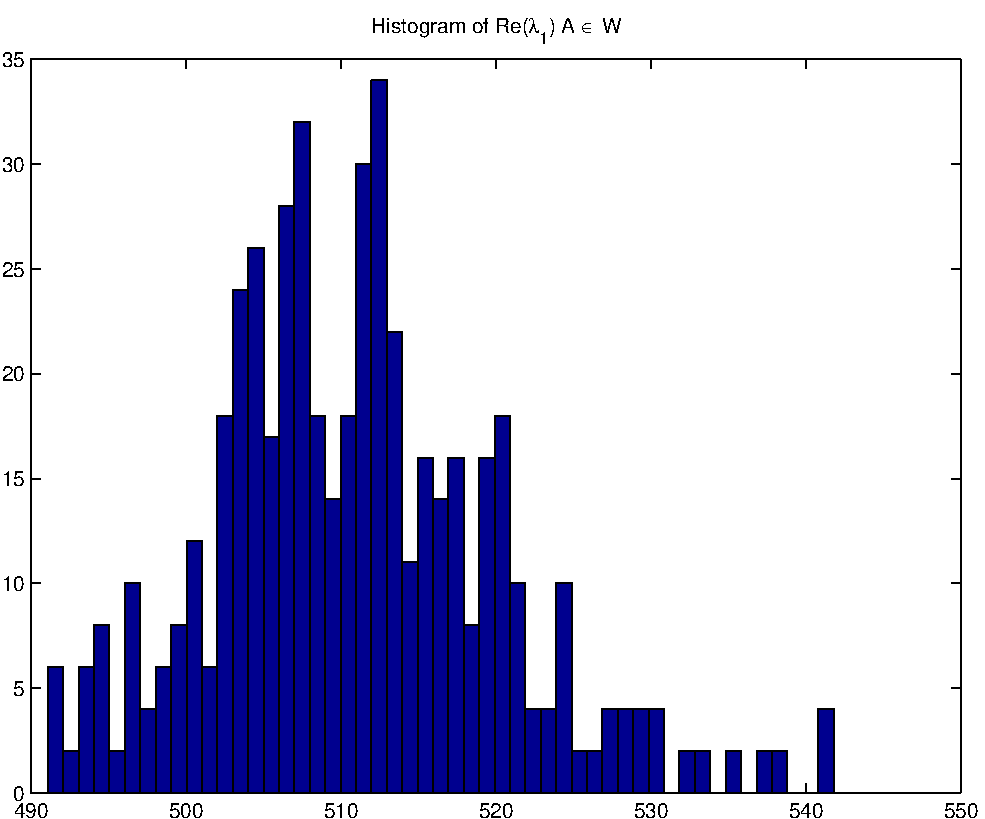
\includegraphics[width=10.0cm,height=10.0cm]{Re_TraceyWidom.pdf}

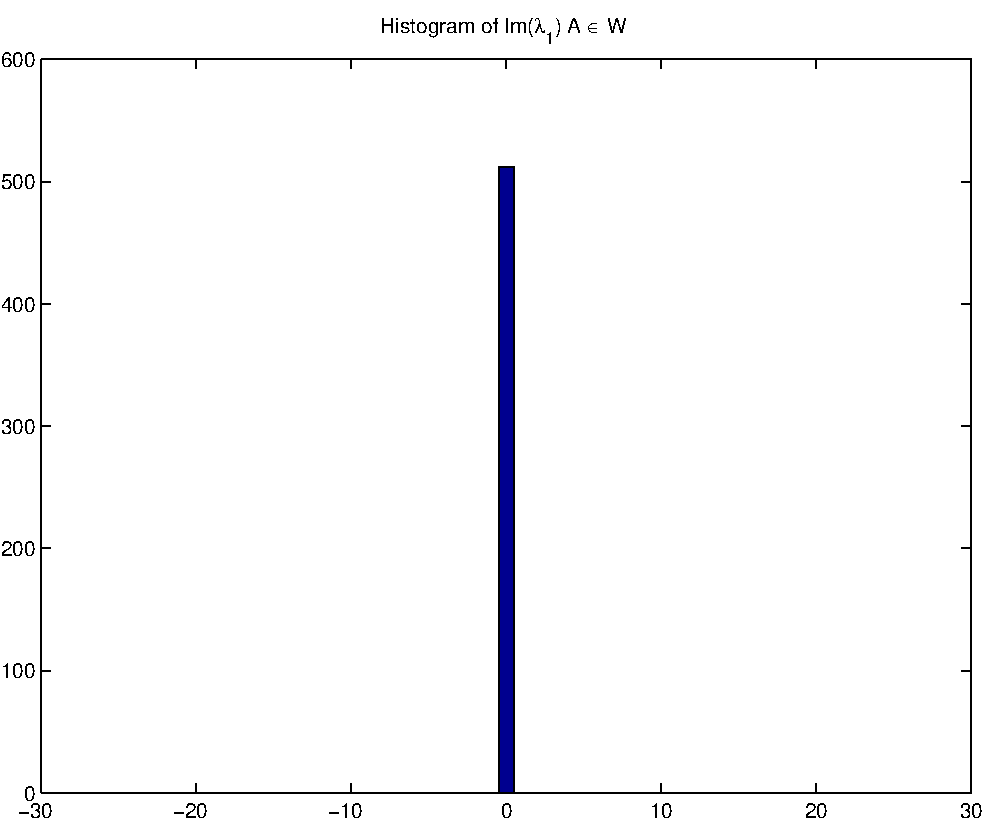
\includegraphics[width=10.0cm,height=10.0cm]{Im_TraceyWidom.pdf}

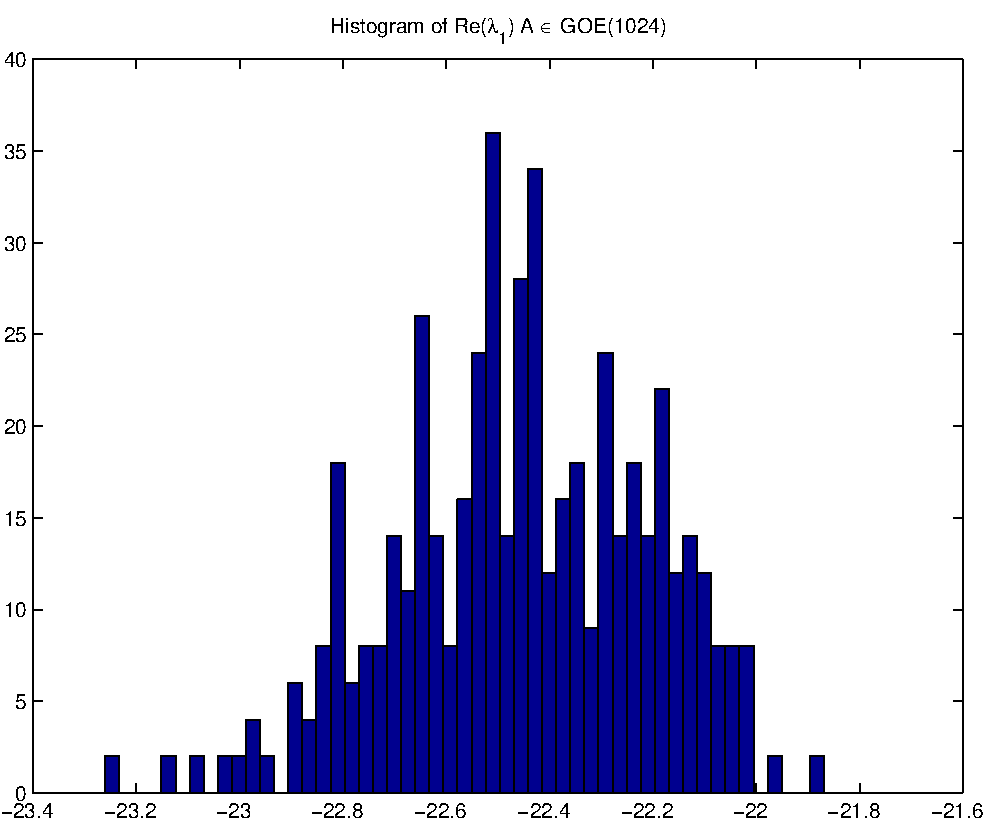
\includegraphics[width=10.0cm,height=10.0cm]{Re_Winger.pdf}

\includegraphics[width=10.0cm,height=10.0cm]{Im_Winger.pdf}

QueryPerformanceCounter  =  +4.797
\subsubsection{Approximate Winger Distribution}
\subsubsection{Verfy Winger Law.}
Let $M_n = [X_{ij} ]$ a symmetric n x n matrix with Random entries such that $X_{i,j} = X_{j,i}$, 		  and $X_{i,j}$ are iid $orall i < j,$ and $Xjj$ are iid $orall j  :  ; E[X^2_{ij} ] = 1, & E[X_{ij}] = 0$ 		  and that all moments exists for each of the entries.  		  The eigenvector of this random matrix; $ lambda_1 leq ... leq lambda_n$ depends continuously on $Mn$.
Dimension $n = +512$

\includegraphics[width=10.0cm,height=10.0cm]{Re_lambda_n.pdf}

\includegraphics[width=10.0cm,height=10.0cm]{Im_lambda_n.pdf}

QueryPerformanceCounter  =  +2.699
\subsubsection{Matrix Exponential }
$SPD Matrix = \left(
\begin{array}{
cccccccc}
+10.539 & -0.499 & -0.010 & +0.368 & +0.465 & -0.492 & -0.126 & +0.437 \\
-0.499 & +7.286 & +0.365 & -0.481 & -0.337 & -0.466 & +0.279 & +0.056 \\
-0.010 & +0.365 & +6.705 & -0.205 & +0.467 & +0.131 & +0.077 & -0.089 \\
+0.368 & -0.481 & -0.205 & +6.496 & -0.402 & -0.209 & +0.043 & -0.041 \\
+0.465 & -0.337 & +0.467 & -0.402 & +4.578 & +0.272 & +0.289 & -0.285 \\
-0.492 & -0.466 & +0.131 & -0.209 & +0.272 & +8.181 & +0.343 & -0.244 \\
-0.126 & +0.279 & +0.077 & +0.043 & +0.289 & +0.343 & +5.938 & -0.212 \\
+0.437 & +0.056 & -0.089 & -0.041 & -0.285 & -0.244 & -0.212 & +9.691 \\
\end{array}
\right)$ \newline 

$SPD Eigs = \left(
\begin{array}{
cccccccc}
(+10.93611,+0.00000) & (+9.60778,+0.00000) & (+4.23666,+0.00000) & (+8.36911,+0.00000) & (+7.56229,+0.00000) & (+5.82791,+0.00000) & (+6.54198,+0.00000) & (+6.33139,+0.00000) \\
\end{array}
\right)$ \newline 

$exp(SPD) = \left(
\begin{array}{
cccccccc}
+47863.969 & -6460.093 & -1078.770 & +4706.958 & +2535.224 & -8475.398 & -2406.368 & +12977.552 \\
-6460.093 & +2780.574 & +516.920 & -1069.918 & -548.083 & -109.707 & +386.466 & -807.216 \\
-1078.770 & +516.920 & +1015.281 & -385.755 & +176.069 & +458.541 & +212.284 & -859.022 \\
+4706.958 & -1069.918 & -385.755 & +1267.210 & +111.181 & -1018.272 & -287.809 & +1036.628 \\
+2535.224 & -548.083 & +176.069 & +111.181 & +413.265 & +135.193 & +45.490 & -502.411 \\
-8475.398 & -109.707 & +458.541 & -1018.272 & +135.193 & +5613.026 & +968.003 & -4270.737 \\
-2406.368 & +386.466 & +212.284 & -287.809 & +45.490 & +968.003 & +632.432 & -1645.725 \\
+12977.552 & -807.216 & -859.022 & +1036.628 & -502.411 & -4270.737 & -1645.725 & +19362.944 \\
\end{array}
\right)$ \newline 

$exp(SPD) eigs = \left(
\begin{array}{
cccccccc}
(+56168.17045,+0.00000) & (+14880.07985,+0.00000) & (+4311.77579,+0.00000) & (+1924.25027,+0.00000) & (+69.17669,+0.00000) & (+339.64809,+0.00000) & (+693.66208,+0.00000) & (+561.93669,+0.00000) \\
\end{array}
\right)$ \newline 

$log(exp(SPD) eigs)  = \left(
\begin{array}{
cccccccc}
(+10.93611,+0.00000) & (+9.60778,+0.00000) & (+8.36911,+0.00000) & (+7.56229,+0.00000) & (+4.23666,+0.00000) & (+5.82791,+0.00000) & (+6.54198,+0.00000) & (+6.33139,+0.00000) \\
\end{array}
\right)$ \newline 

$exp(Id) = \left(
\begin{array}{
cccccccc}
+2.718 & +0.000 & +0.000 & +0.000 & +0.000 & +0.000 & +0.000 & +0.000 \\
+0.000 & +2.718 & +0.000 & +0.000 & +0.000 & +0.000 & +0.000 & +0.000 \\
+0.000 & +0.000 & +2.718 & +0.000 & +0.000 & +0.000 & +0.000 & +0.000 \\
+0.000 & +0.000 & +0.000 & +2.718 & +0.000 & +0.000 & +0.000 & +0.000 \\
+0.000 & +0.000 & +0.000 & +0.000 & +2.718 & +0.000 & +0.000 & +0.000 \\
+0.000 & +0.000 & +0.000 & +0.000 & +0.000 & +2.718 & +0.000 & +0.000 \\
+0.000 & +0.000 & +0.000 & +0.000 & +0.000 & +0.000 & +2.718 & +0.000 \\
+0.000 & +0.000 & +0.000 & +0.000 & +0.000 & +0.000 & +0.000 & +2.718 \\
\end{array}
\right)$ \newline 

$exp(Id) eigs = \left(
\begin{array}{
cccccccc}
(+2.71828,+0.00000) & (+2.71828,+0.00000) & (+2.71828,+0.00000) & (+2.71828,+0.00000) & (+2.71828,+0.00000) & (+2.71828,+0.00000) & (+2.71828,+0.00000) & (+2.71828,+0.00000) \\
\end{array}
\right)$ \newline 

$log(exp(Id) eigs)  = \left(
\begin{array}{
cccccccc}
(+1.00000,+0.00000) & (+1.00000,+0.00000) & (+1.00000,+0.00000) & (+1.00000,+0.00000) & (+1.00000,+0.00000) & (+1.00000,+0.00000) & (+1.00000,+0.00000) & (+1.00000,+0.00000) \\
\end{array}
\right)$ \newline 

For $n  \in  \dblz [16,128)$ we calculate  $|( SPD(n) Eigs - log(exp(SPD(n)) eigs)|_{l^2}$

$|( SPD(n) Eigs - log(exp(SPD(n)) eigs)|_{l^2} = \left(
\begin{array}{
cccccccccccccccccccccccccccccccccccccccccccccccccccccccccccccccccccccccccccccccccccccccccccccccccccccccccccccccc}
(+5.36543,+0.00000) & (+5.36543,+0.00000) & (+5.36543,+0.00000) & (+5.36543,+0.00000) & (+5.36543,+0.00000) & (+5.36543,+0.00000) & (+5.36543,+0.00000) & (+5.36543,+0.00000) & (+5.36543,+0.00000) & (+5.36543,+0.00000) & (+5.36543,+0.00000) & (+5.36543,+0.00000) & (+5.36543,+0.00000) & (+5.36543,+0.00000) & (+5.36543,+0.00000) & (+5.36543,+0.00000) & (+5.36543,+0.00000) & (+5.36543,+0.00000) & (+5.36543,+0.00000) & (+5.36543,+0.00000) & (+5.36543,+0.00000) & (+5.36543,+0.00000) & (+5.36543,+0.00000) & (+5.36543,+0.00000) & (+5.36543,+0.00000) & (+5.36543,+0.00000) & (+5.36543,+0.00000) & (+5.36543,+0.00000) & (+5.36543,+0.00000) & (+5.36543,+0.00000) & (+5.36543,+0.00000) & (+5.36543,+0.00000) & (+5.36543,+0.00000) & (+5.36543,+0.00000) & (+5.36543,+0.00000) & (+5.36543,+0.00000) & (+5.36543,+0.00000) & (+5.36543,+0.00000) & (+5.36543,+0.00000) & (+5.36543,+0.00000) & (+5.36543,+0.00000) & (+5.36543,+0.00000) & (+5.36543,+0.00000) & (+5.36543,+0.00000) & (+5.36543,+0.00000) & (+5.36543,+0.00000) & (+5.36543,+0.00000) & (+5.36543,+0.00000) & (+0.00000,+0.00000) & (+0.00000,+0.00000) & (+0.00000,+0.00000) & (+0.00000,+0.00000) & (+0.00000,+0.00000) & (+0.00000,+0.00000) & (+0.00000,+0.00000) & (+0.00000,+0.00000) & (+0.00000,+0.00000) & (+0.00000,+0.00000) & (+0.00000,+0.00000) & (+0.00000,+0.00000) & (+0.00000,+0.00000) & (+0.00000,+0.00000) & (+0.00000,+0.00000) & (+0.00000,+0.00000) & (+0.00000,+0.00000) & (+0.00000,+0.00000) & (+0.00000,+0.00000) & (+0.00000,+0.00000) & (+0.00000,+0.00000) & (+0.00000,+0.00000) & (+0.00000,+0.00000) & (+0.00000,+0.00000) & (+0.00000,+0.00000) & (+0.00000,+0.00000) & (+0.00000,+0.00000) & (+0.00000,+0.00000) & (+0.00000,+0.00000) & (+0.00000,+0.00000) & (+0.00000,+0.00000) & (+0.00000,+0.00000) & (+0.00000,+0.00000) & (+0.00000,+0.00000) & (+0.00000,+0.00000) & (+0.00000,+0.00000) & (+0.00000,+0.00000) & (+0.00000,+0.00000) & (+0.00000,+0.00000) & (+0.00000,+0.00000) & (+0.00000,+0.00000) & (+0.00000,+0.00000) & (+0.00000,+0.00000) & (+0.00000,+0.00000) & (+0.00000,+0.00000) & (+0.00000,+0.00000) & (+0.00000,+0.00000) & (+0.00000,+0.00000) & (+0.00000,+0.00000) & (+0.00000,+0.00000) & (+0.00000,+0.00000) & (+0.00000,+0.00000) & (+0.00000,+0.00000) & (+0.00000,+0.00000) & (+0.00000,+0.00000) & (+0.00000,+0.00000) & (+0.00000,+0.00000) & (+0.00000,+0.00000) & (+0.00000,+0.00000) & (+0.00000,+0.00000) & (+0.00000,+0.00000) & (+0.00000,+0.00000) & (+0.00000,+0.00000) & (+0.00000,+0.00000) \\
\end{array}
\right)$ \newline 

QueryPerformanceCounter  =  +0.00933
The sample size generated for this run is 100000.

\newpage
uniform \begin{tabular}{|c|c|c|c|}  mean & variance & skewness & kurtosis \\  \hline
$\mu_1 = +0.50030$ & $\mu_2 = +0.08353$ & $\mu_3 = +0.00339$ & $\mu_4 =+1.80113$ \\
\end{tabular}

\includegraphics[width=5cm,height=5cm]{uniform.pdf}

cauchy \begin{tabular}{|c|c|c|c|}  mean & variance & skewness & kurtosis \\  \hline
$\mu_1 = +0.44288$ & $\mu_2 = +0.05341$ & $\mu_3 = +0.63935$ & $\mu_4 =+3.28094$ \\
\end{tabular}

\includegraphics[width=5cm,height=5cm]{cauchy.pdf}

exponential \begin{tabular}{|c|c|c|c|}  mean & variance & skewness & kurtosis \\  \hline
$\mu_1 = +1.99647$ & $\mu_2 = +3.99339$ & $\mu_3 = +2.03097$ & $\mu_4 =+9.30842$ \\
\end{tabular}

\includegraphics[width=5cm,height=5cm]{exponential.pdf}

\newpage
gamma \begin{tabular}{|c|c|c|c|}  mean & variance & skewness & kurtosis \\  \hline
$\mu_1 = +1.88789$ & $\mu_2 = +1.87354$ & $\mu_3 = +1.47483$ & $\mu_4 =+6.40880$ \\
\end{tabular}

\includegraphics[width=5cm,height=5cm]{gamma.pdf}

GIG \begin{tabular}{|c|c|c|c|}  mean & variance & skewness & kurtosis \\  \hline
$\mu_1 = +0.81608$ & $\mu_2 = +12.40951$ & $\mu_3 = +15.79782$ & $\mu_4 =+333.58392$ \\
\end{tabular}

\includegraphics[width=5cm,height=5cm]{GIG.pdf}

normal-box-muller \begin{tabular}{|c|c|c|c|}  mean & variance & skewness & kurtosis \\  \hline
$\mu_1 = -0.00181$ & $\mu_2 = +0.99640$ & $\mu_3 = -0.00050$ & $\mu_4 =+3.00088$ \\
\end{tabular}

\includegraphics[width=5cm,height=5cm]{normal-box-muller.pdf}

\newpage
normal-inverse-approximation \begin{tabular}{|c|c|c|c|}  mean & variance & skewness & kurtosis \\  \hline
$\mu_1 = +0.00230$ & $\mu_2 = +1.00486$ & $\mu_3 = +0.01163$ & $\mu_4 =+2.99254$ \\
\end{tabular}

\includegraphics[width=5cm,height=5cm]{normal-inverse-approximation.pdf}

pareto \begin{tabular}{|c|c|c|c|}  mean & variance & skewness & kurtosis \\  \hline
$\mu_1 = +3184578.26493$ & $\mu_2 = +888468246174112900.00000$ & $\mu_3 = +315.36997$ & $\mu_4 =+99629.09819$ \\
\end{tabular}

\includegraphics[width=5cm,height=5cm]{pareto.pdf}

poisson \begin{tabular}{|c|c|c|c|}  mean & variance & skewness & kurtosis \\  \hline
$\mu_1 = +1.10787$ & $\mu_2 = +0.13493$ & $\mu_3 = +3.90287$ & $\mu_4 =+20.70306$ \\
\end{tabular}

\includegraphics[width=5cm,height=5cm]{poisson.pdf}

\newpage
beta \begin{tabular}{|c|c|c|c|}  mean & variance & skewness & kurtosis \\  \hline
$\mu_1 = +0.33362$ & $\mu_2 = +0.12713$ & $\mu_3 = +0.67738$ & $\mu_4 =+1.90380$ \\
\end{tabular}

\includegraphics[width=5cm,height=5cm]{beta.pdf}

QueryPerformanceCounter  =  +10.93021
\subsubsection{Multiclass Support Vector Machine }
\begin{itemize}
\item Number or training points = 1024
\item Feature dimension = 3
\item Number or classes = 3
\end{itemize}
{The mean vectors of the 3 classes}

$\mu_1 = \left(
\begin{array}{
ccc}
+1.90000 & +0.10000 & +0.10000 \\
\end{array}
\right)$ \newline 

$\mu_2 = \left(
\begin{array}{
ccc}
+0.10000 & +1.90000 & +0.10000 \\
\end{array}
\right)$ \newline 

$\mu_3 = \left(
\begin{array}{
ccc}
+0.00000 & +0.00000 & +1.90000 \\
\end{array}
\right)$ \newline 

A random SPD covairance matrix is generated for each of the classes.\newline

$\rho_1 = \left(
\begin{array}{
ccc}
+2.511 & -0.093 & -0.244 \\
-0.093 & +2.713 & -0.260 \\
-0.244 & -0.260 & +1.607 \\
\end{array}
\right)$ \newline 

$\rho_2 = \left(
\begin{array}{
ccc}
+2.050 & -0.265 & -0.070 \\
-0.265 & +2.232 & +0.440 \\
-0.070 & +0.440 & +2.654 \\
\end{array}
\right)$ \newline 

$\rho_3 = \left(
\begin{array}{
ccc}
+3.801 & +0.257 & -0.091 \\
+0.257 & +3.373 & -0.468 \\
-0.091 & -0.468 & +2.083 \\
\end{array}
\right)$ \newline 

Verify $L_1$ condition number of covariance. The diagonal entries of the matrix have the form $(0.5 + U(0,1) )*dim(Dom(Cov))$
The lower-diagonal entries take the form $U(0,1) - 0.5$. 
The $L_1$ condition numbers are :
\begin{itemize}
\item +2.365
\item +1.763
\item +2.369
\end{itemize}
\includegraphics[width=10.0cm,height=10.0cm]{rv1_corr.pdf}

\includegraphics[width=10.0cm,height=10.0cm]{rv2_corr.pdf}

\includegraphics[width=10.0cm,height=10.0cm]{rv3_corr.pdf}

\includegraphics[width=10.0cm,height=10.0cm]{trainingPoints.pdf}

These are the SVM parameters - the RBF kernel is used\begin{itemize}
\item allOutlierFraction=0.05
\item mixingCoeff=0.3
\item smoThresh=1.0/10000.0
\item sigma=1
\end{itemize}
\includegraphics[width=10.0cm,height=10.0cm]{testPoints.pdf}

The marginal sample moments (mean var skew kurtosis) for training points.\newline
\begin{tabular}{ c |  c  c  c  c}
Feature & $\mu_1$ & $\mu_2$ & $\mu_3$ & $\mu_4$ \\
0 & +0.669 & +1.322 & +0.171& +2.323 \\
\hline
1 & +0.702 & +1.240 & +0.209& +2.211 \\
\hline
2 & +0.700 & +1.138 & +0.383& +2.335 \\
\hline
\end{tabular}
\newline
The marginal sample moments (mean var skew kurtosis) for test points.\newline
\begin{tabular}{ c | c  c  c  c}
Feature & $\mu_1$ & $\mu_2$ & $\mu_3$ & $\mu_4$ \\
0 & +0.676 & +1.234 & +0.292& +2.426\\
\hline
1 & +0.668 & +1.239 & +0.265& +2.214\\
\hline
2 & +0.718 & +1.096 & +0.349& +2.325\\
\hline
\end{tabular}\newline
\includegraphics[width=10.0cm,height=10.0cm]{classDiffs.pdf}

The error rate for this run is +0.090\newline
QueryPerformanceCounter  =  +6.402
\subsubsection{Semidefinite Programming SDPA}
QueryPerformanceCounter  =  +0.005
\end{document}
